\section{Intermediate $\AR$s with $3 < \AR < 4.75$}
\label{sec:int}

We now focus on the horizontal $n=1$ branch, dominated by LE vortex shedding (see figure~\ref{fig:StLAR}), corresponding to the aspect ratio range $3 \leq \AR \leq 4.75$. Within this regime, we select $\AR=4$ and $\AR=4.5$ as representative cases. For these aspect ratios, the secondary bifurcation is triggered by a two-dimensional instability that leads to a deviated wake. To the best of our knowledge, this phenomenon has not been previously reported for symmetric two-dimensional bluff bodies.

\subsection{A $2D$ bifurcation}

\subsubsection{Non linear simulations}


\begin{figure}
  \centering
  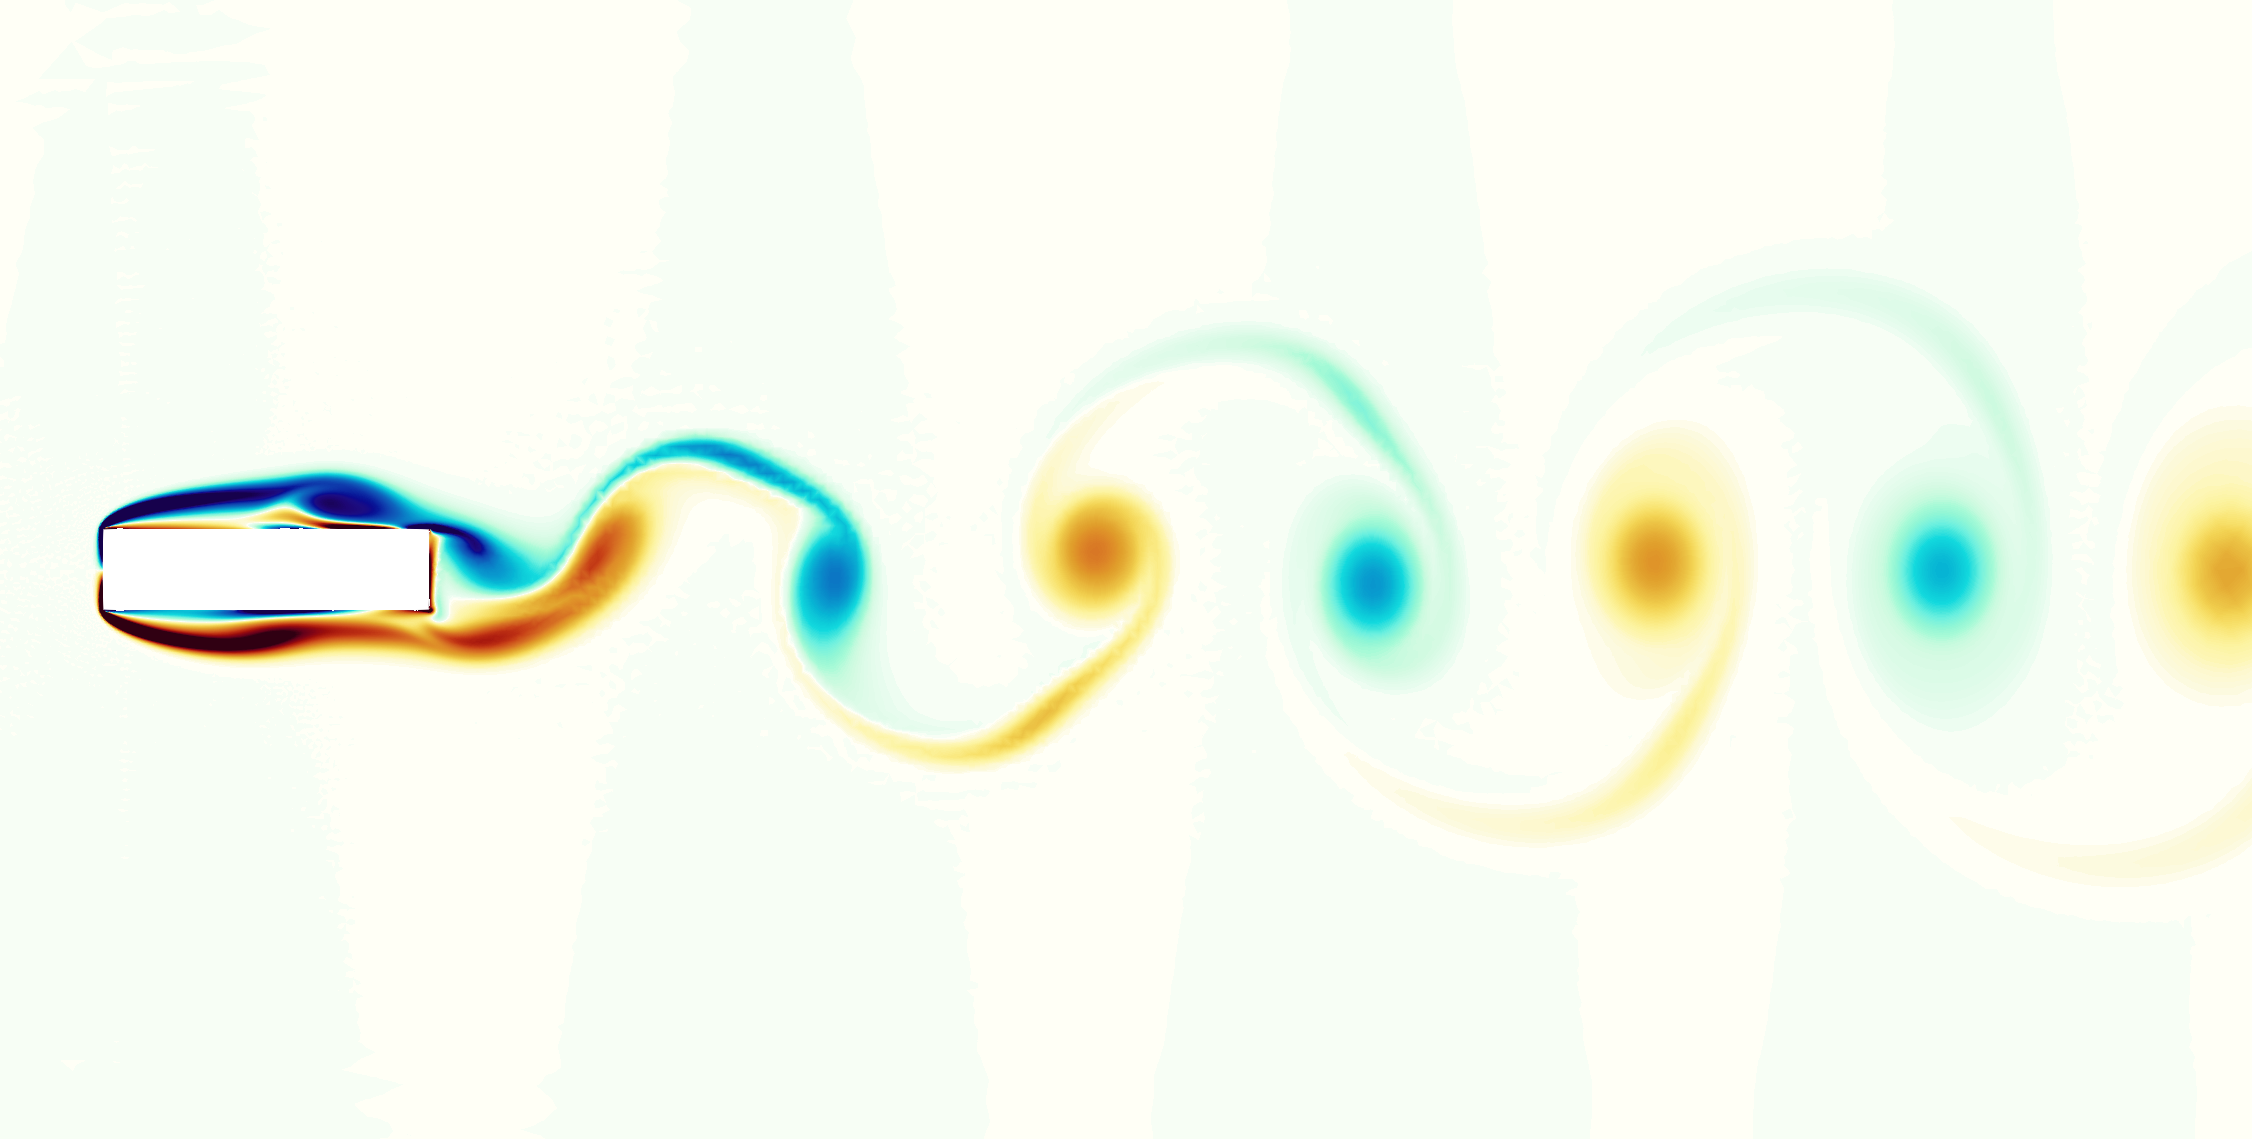
\includegraphics[trim={0 100 0 100},clip,width=0.49\textwidth]{./fig/vort_Re425_25.png}
  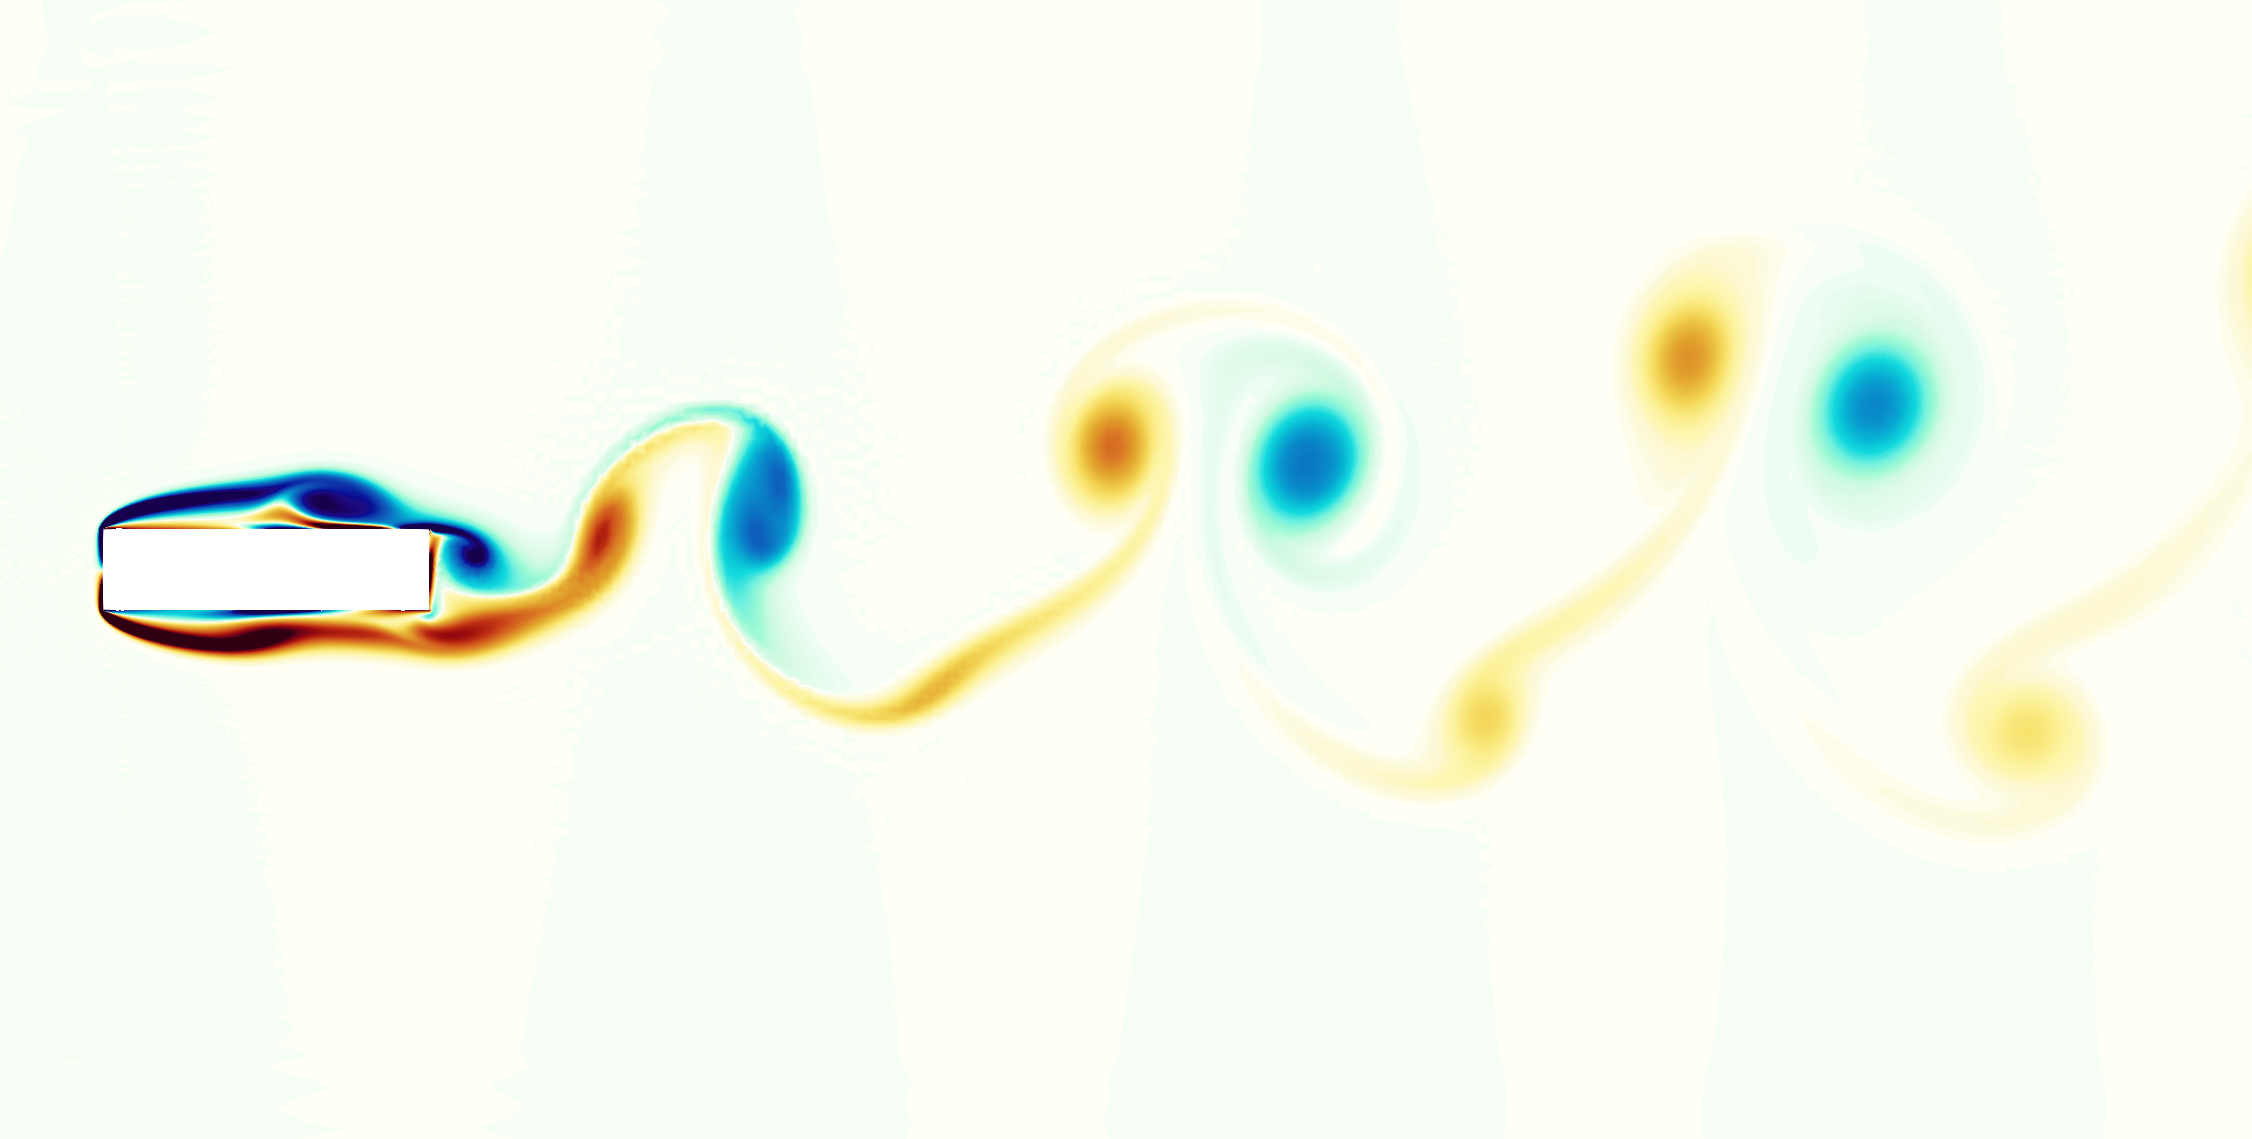
\includegraphics[trim={0 100 0 100},clip,width=0.49\textwidth]{./fig/vort_Re450_25.png}  
  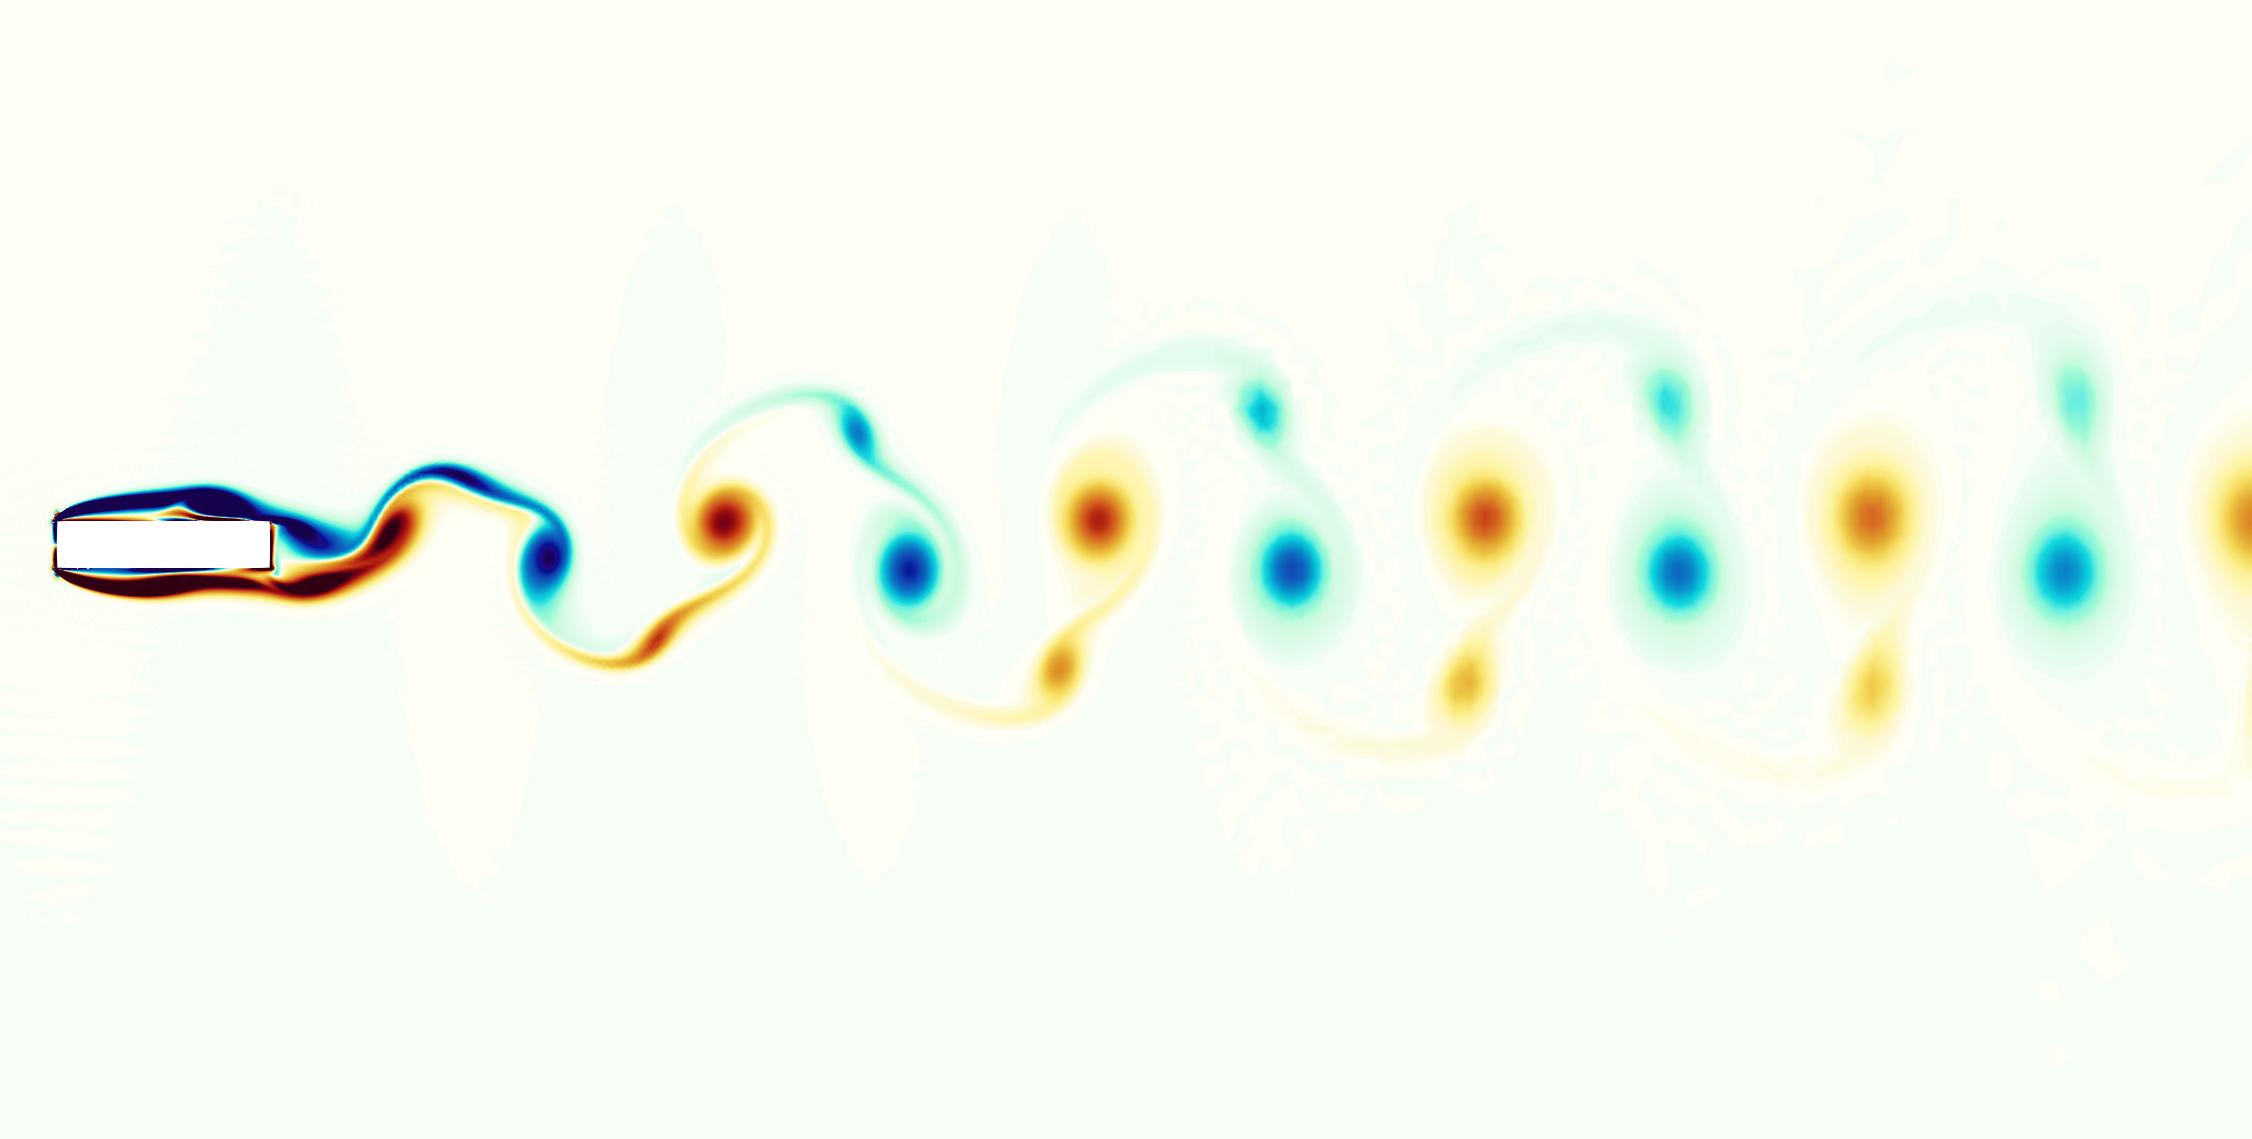
\includegraphics[trim={0 100 0 100},clip,width=0.49\textwidth]{./fig/AR4p5/vort_Re430_25.png}
  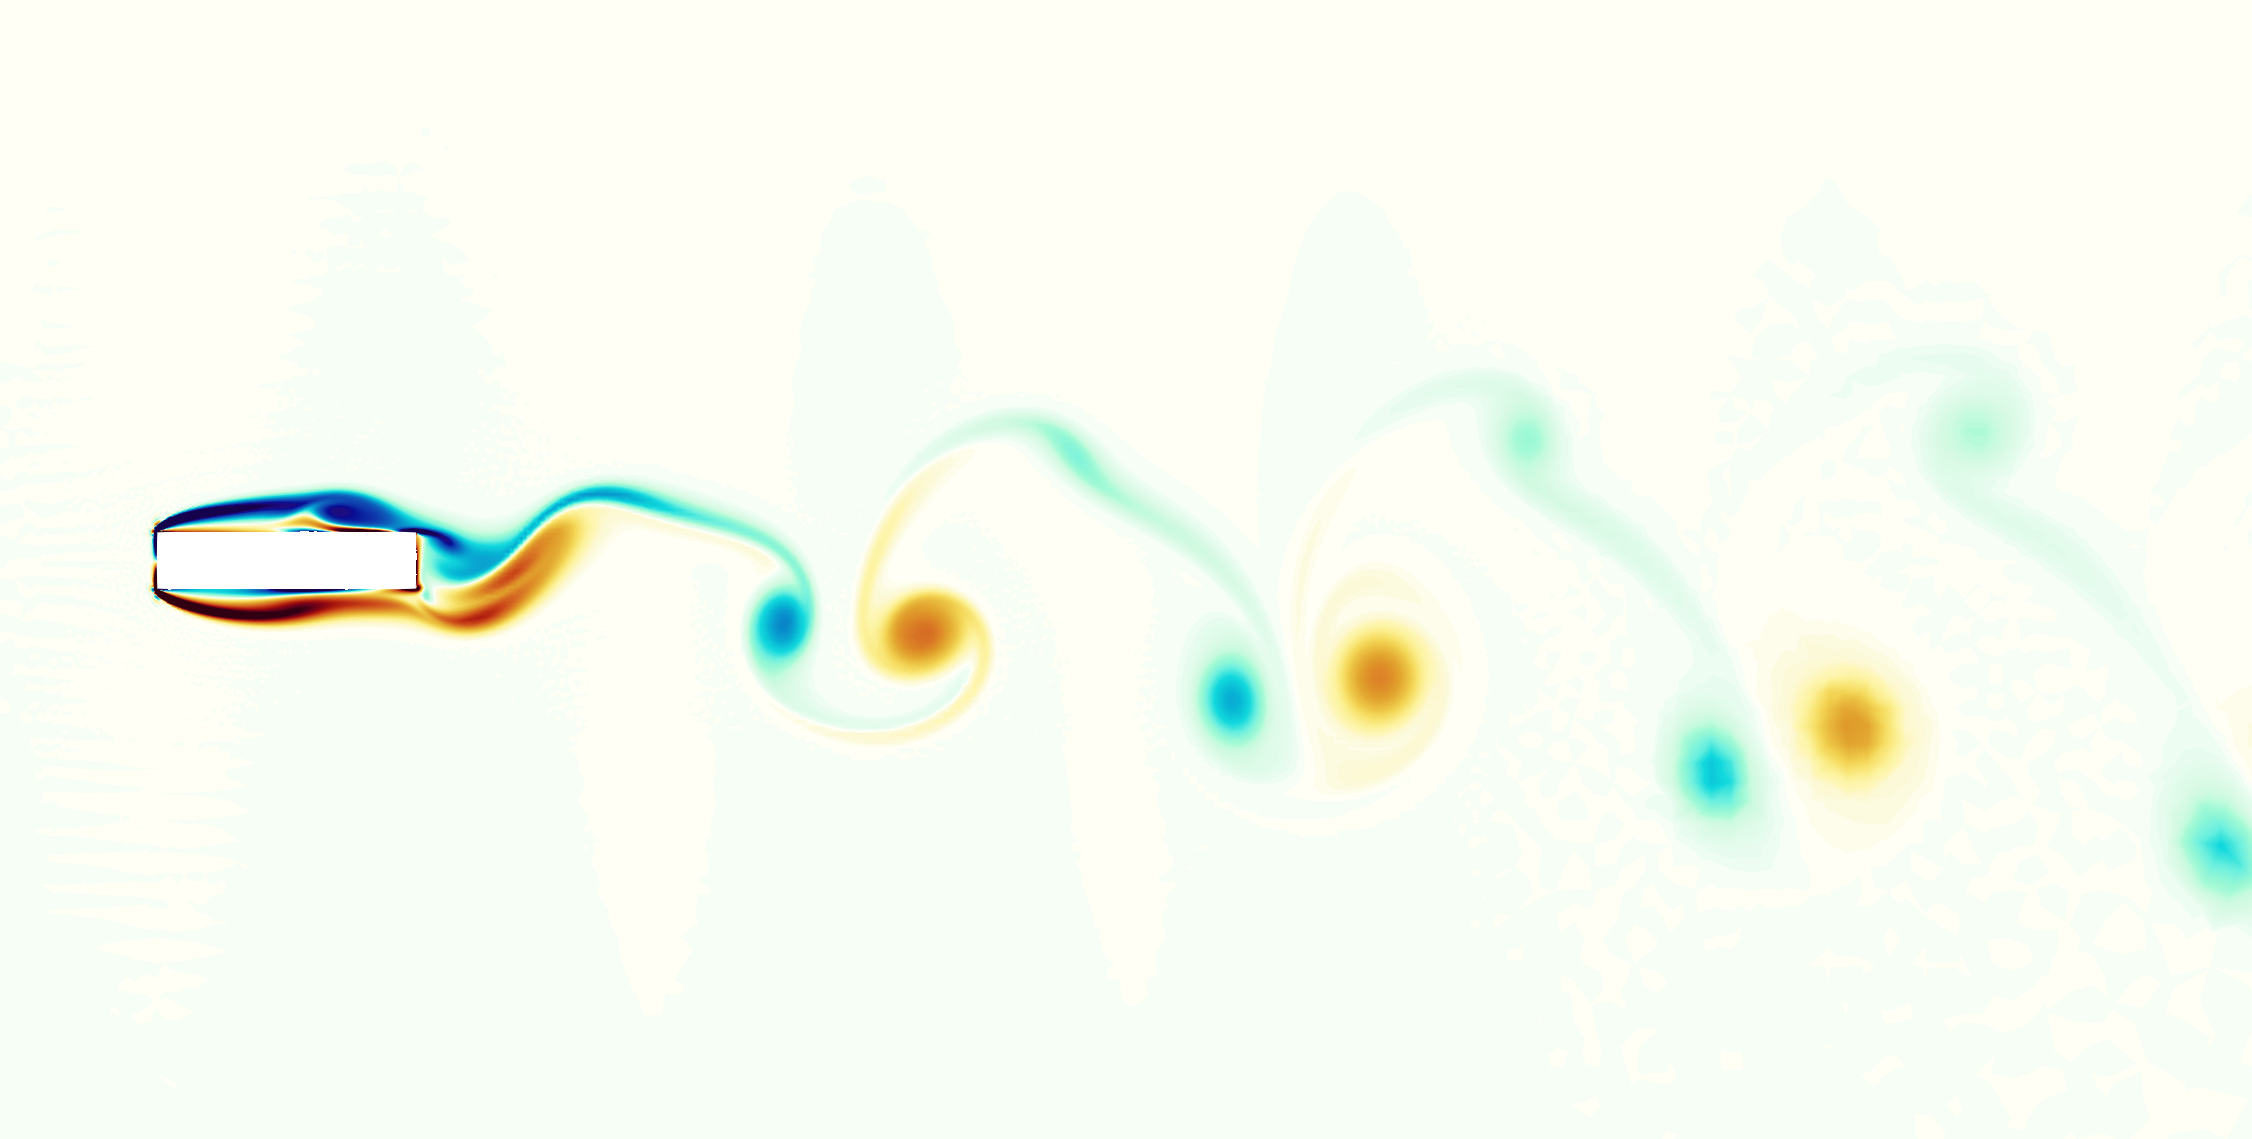
\includegraphics[trim={0 100 0 100},clip,width=0.49\textwidth]{./fig/AR4p5/vort_Re450_25.png}
  \caption{Instantaneous snapshots for $\AR=4$ at $Re=425$ (top left) and $Re=450$ (top right), and $\AR=4.5$ at $Re=430$ (bottom left) at $Re=450$ (bottom right).}
  \label{fig:snap_ar4_ar4p5}
\end{figure}

Nonlinear simulations reveal that as the Reynolds number increases to the critical value $Re = Re_{c2}$, the 2D periodic base flow becomes unstable to 2D perturbations, undergoing a synchronous bifurcation. The resulting flow maintains the original temporal periodicity but develops a distinct slanted wake. This transition is illustrated in figure \ref{fig:snap_ar4_ar4p5}, which shows instantaneous vorticity fields at various Reynolds numbers.

For $Re \le Re_{c2}$ (left panels), the wake remains aligned with the $x$-axis and exhibits the canonical von-K\'{a}rm\'{a}n-like vortex shedding pattern, characterised by alternating vortices of opposite sign shed along the centerline $y=0$. This flow regime, extensively analysed in \cite{chiarini-quadrio-auteri-2022}, is briefly recalled here for completeness. In this parameter range, the dynamics are dominated by leading-edge (LE) vortex shedding, where a single vortex alternately forms on each side of the cylinder. These LE vortices convect downstream and, upon traversing the trailing edge (TE), induce a hyperbolic stagnation point that triggers the subsequent shedding of a TE vortex of opposite sign from the opposing side \citep{chiarini-quadrio-auteri-2022}.
%
Critically, the timing of the LE vortex passing the TE corner is phase-locked with the shedding of the associated TE vortex. The relative phase shift between LE passage and TE shedding exhibits a mild dependence on the aspect ratio, accounting for observed variations in wake topology between the $\AR=4$ and $\AR=4.5$ configurations. Specifically, the LE vortices downstream are markedly attenuated for $\AR=4$ compared to $\AR=4.5$.

Beyond the critical Reynolds number $Re_{c2}$, the flow undergoes a bifurcation characterised by the loss of reflectional symmetry about the centerline $y=0$, leading to a persistent wake deviation. In this regime, the vortex monopoles no longer remain aligned along $y=0$, but are displaced either above or below the centerline. For $\AR=4$, this symmetry-breaking transition occurs at $Re \ge Re_{c2} \approx 435$, wherease for $\AR=4.5$, it manifests at a slightly lower threshold $Re \ge Re_{c2} \approx 417.5$. The direction of wake deflection---upward or downward---is determined by the initial flow conditions and is effectively random.

\begin{figure}
  \centering
  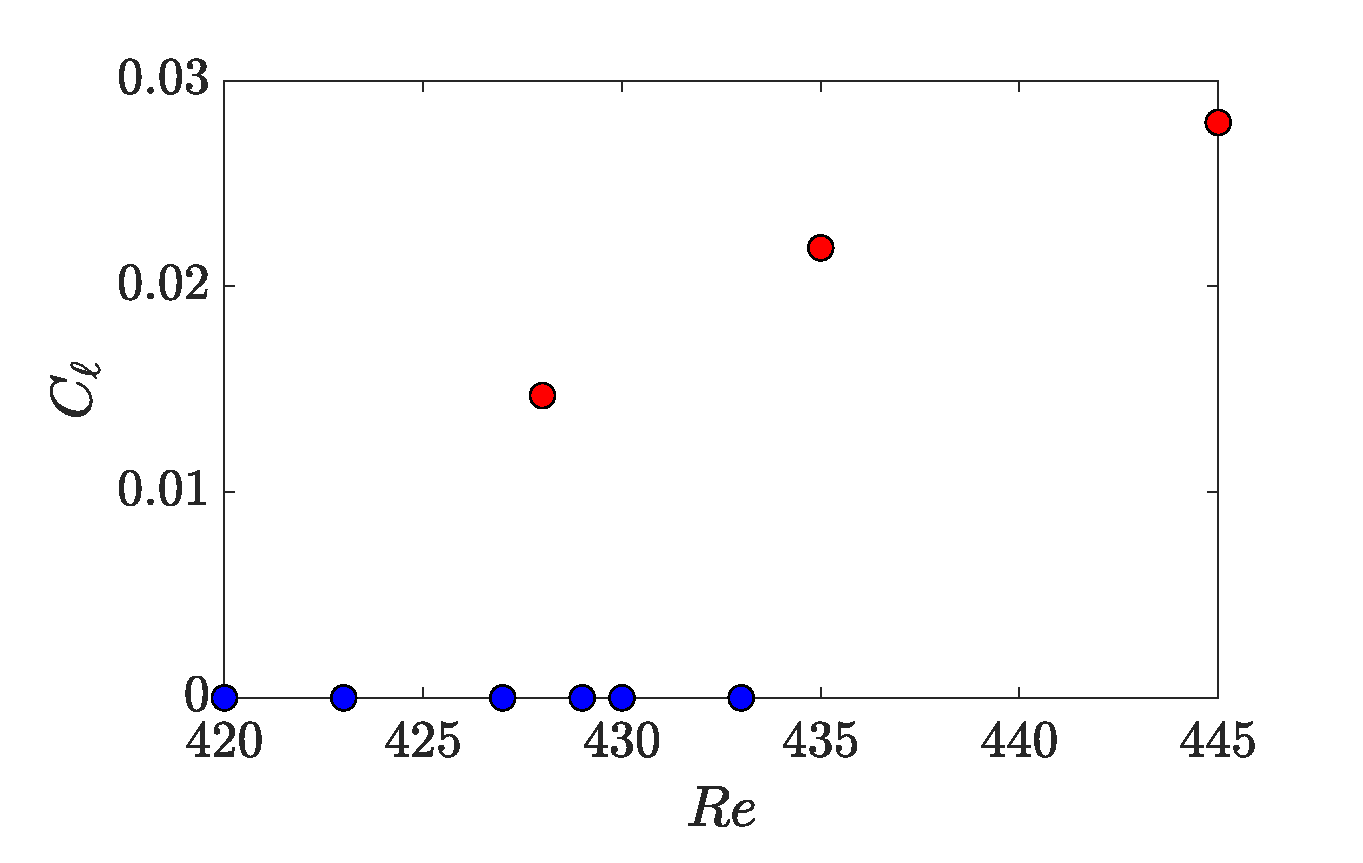
\includegraphics[width=0.49\textwidth]{./fig/AR4_Cl_Re.eps}
  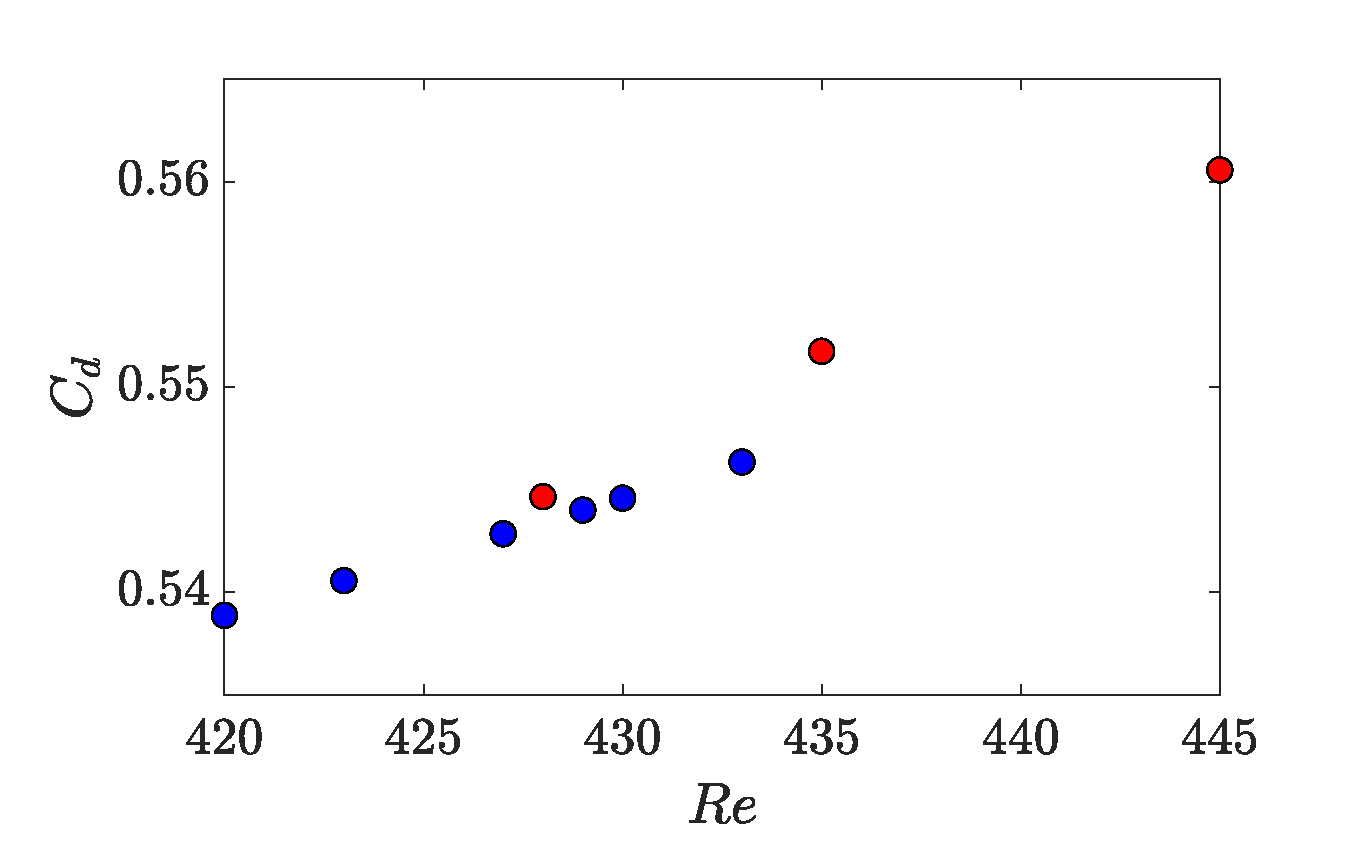
\includegraphics[width=0.49\textwidth]{./fig/AR4_Cd_Re.eps}
  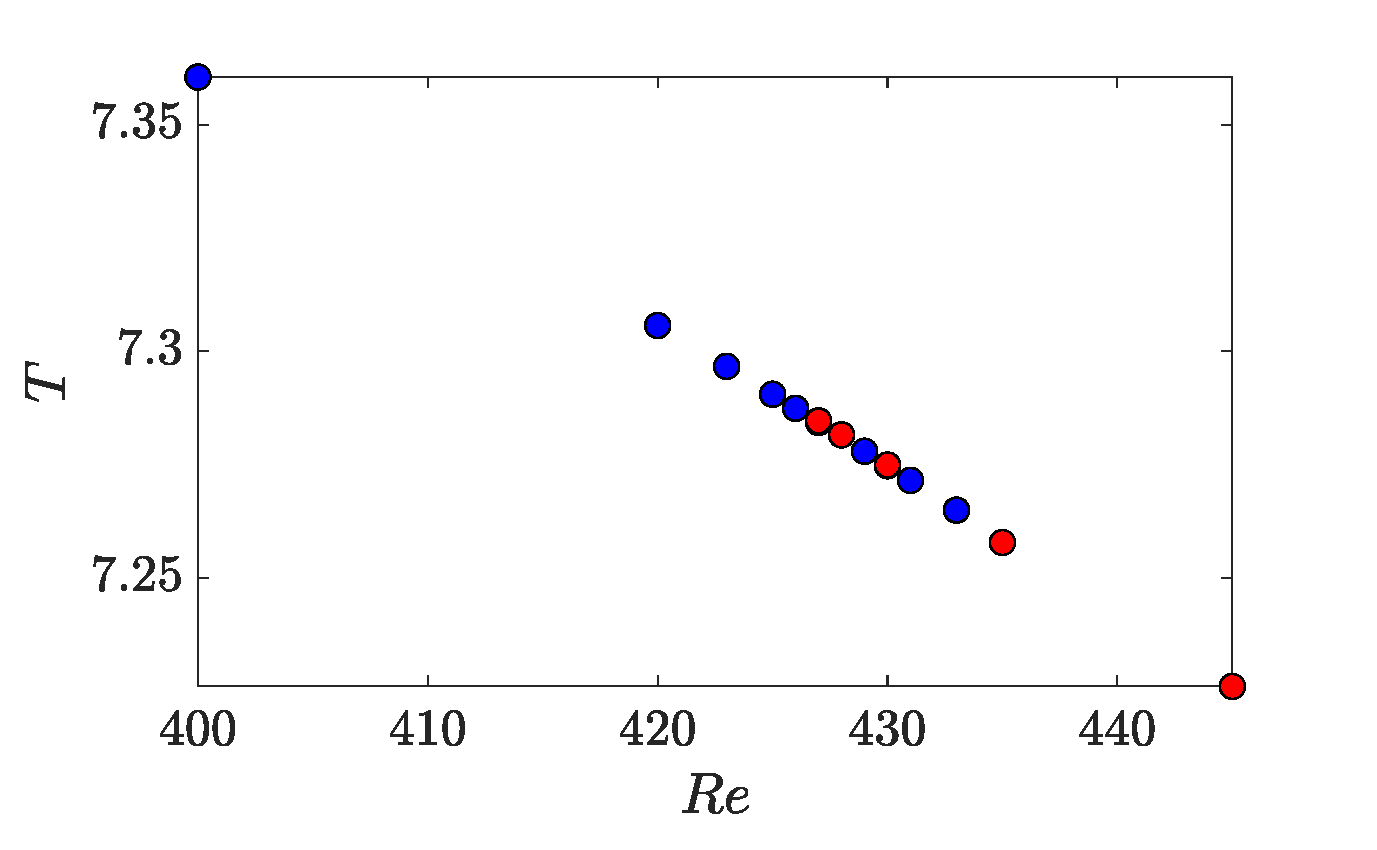
\includegraphics[width=0.49\textwidth]{./fig/AR4_T_Re.eps}
  \caption{Dependence of $C_\ell$, $C_d$ and $T$ on the Reynolds number $Re$. The straight wake for $Re>Re_{c2}$ has been stabilised by means of the BoostConv algorithm.}
  \label{fig:Cl-Cd-AR4}
\end{figure}
%
To further characterise this bifurcation, figure \ref{fig:Cl-Cd-AR4} presents the Reynolds number dependence of the aerodynamic force coefficients---lift $C_\ell$ and drag $C_d$---as well as the flow period $T$ for $\AR=4$. For $Re>Re_{c2}$, the unstable straight-wake solution is stabilised via the BoostConv algorithm. Consistent with flow symmetry, the time-average lift coefficient remains zero $\langle C_\ell \rangle = 0$ for $Re \le Re_{c2}$, while it departs from zero $\langle C_\ell \rangle \neq 0$ for $Re>Re_{c2}$, indicating the symmetry-breaking associated with the bifurcation. In contrast, the drag coefficient exhibits a monotonic increase with Reynolds number across both regimes, with a notably steeper slope in the deviated wake state. Figure \ref{fig:Cl-Cd-AR4}(c) further substantiates the synchronous nature of the bifurcation: the flow period $T$ for both the symmetric and deviated wake solutions collapses onto a single curve, decreasing smoothly with increasing $Re$. The continuous, smooth behaviour of the $C_\ell-Re$ and $C_d-Re$ curves strongly suggests a supercritical or smooth bifurcation. This characterisation will be explored in greater detail in subsequent sections.

\subsubsection{Linear stability analysis}
\begin{figure}
\centering
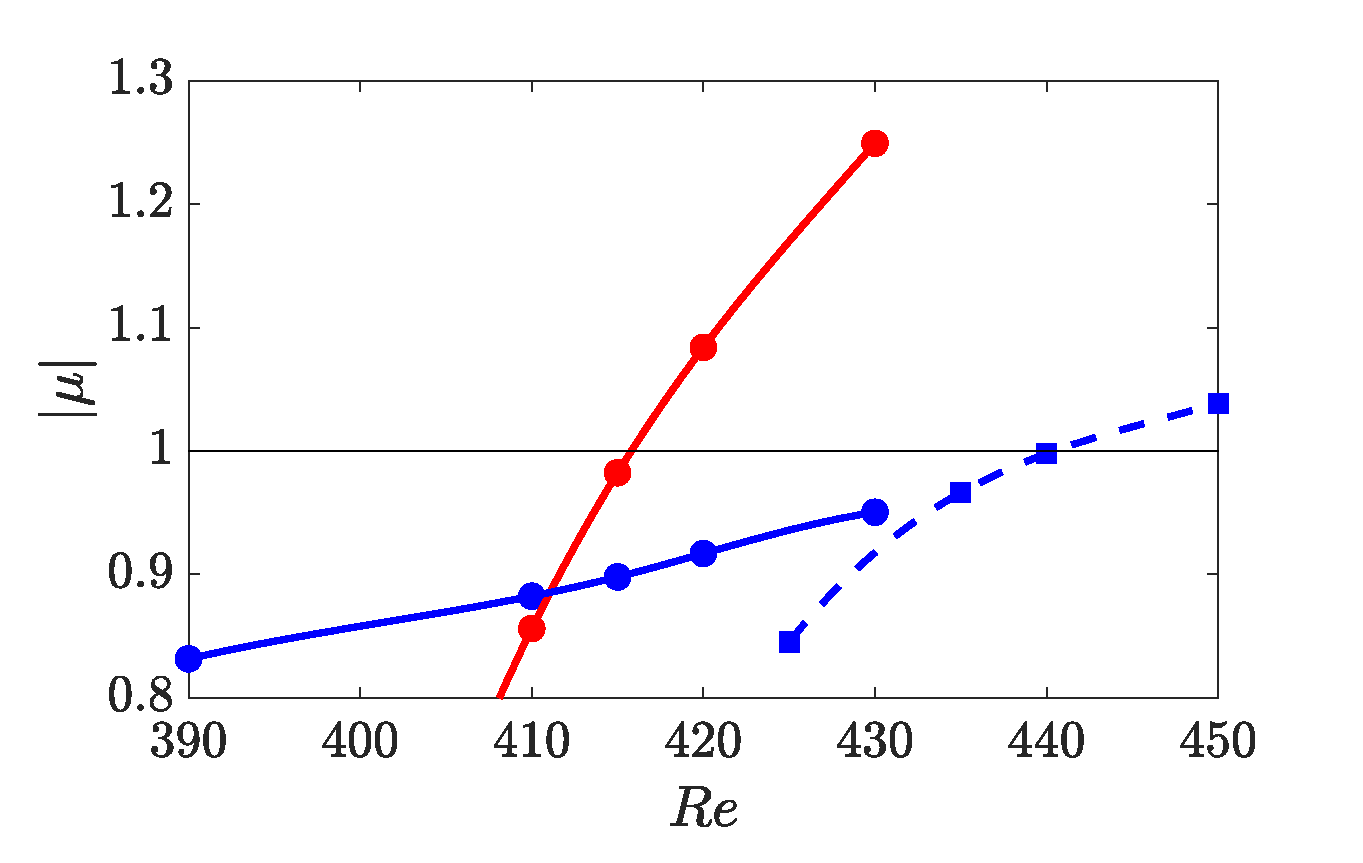
\includegraphics[width=0.49\textwidth]{./fig/AR4p5/multipliers_2D.eps}
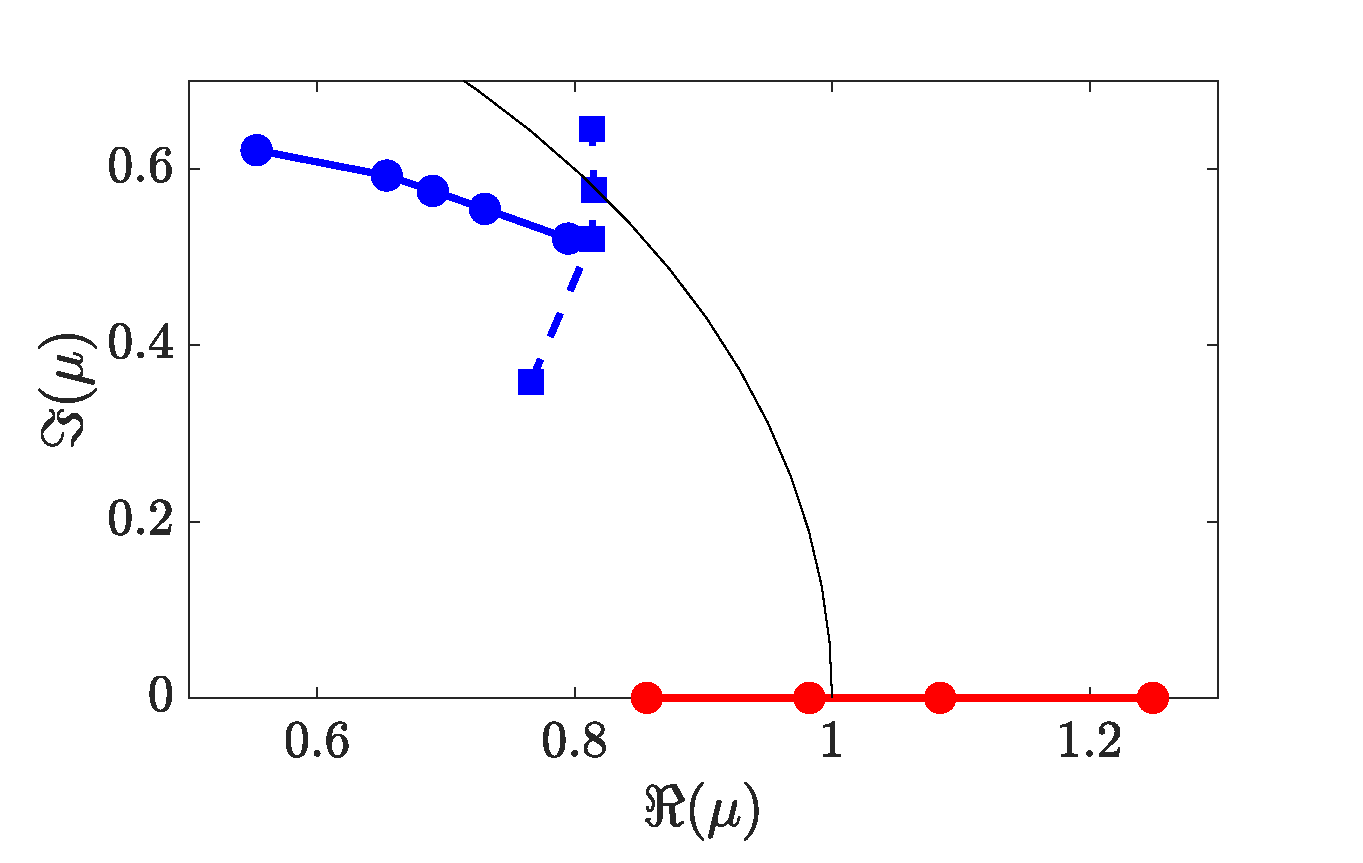
\includegraphics[width=0.49\textwidth]{./fig/AR4p5/multipliers_2D_b.eps}
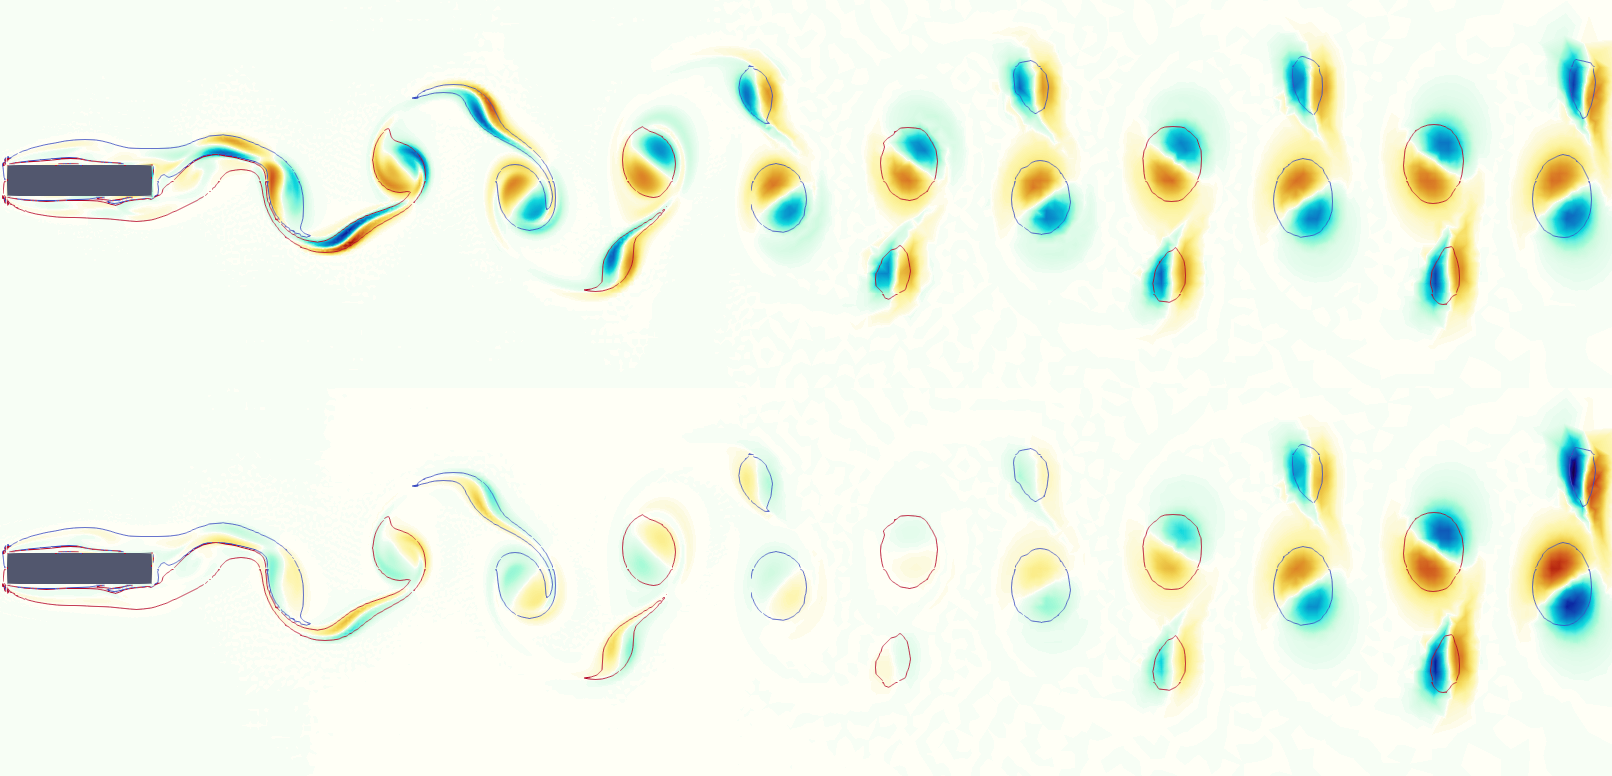
\includegraphics[width=0.7\textwidth]{./fig/AR4p5/omegaz_beta0_Re430_AB.png}
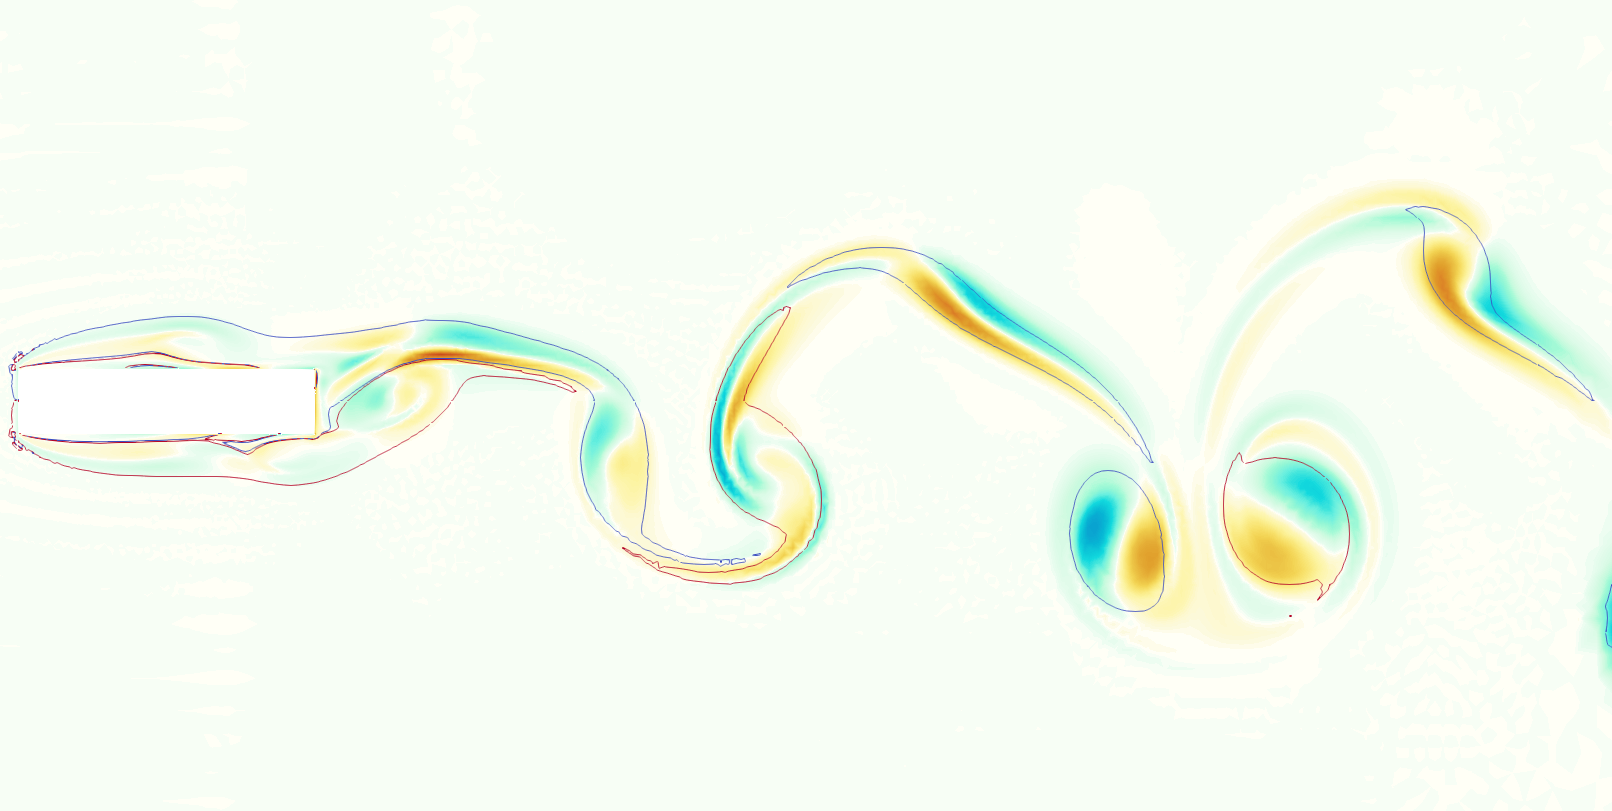
\includegraphics[width=0.7\textwidth]{./fig/AR4p5/Floqetmode_beta_0_Re450_AR4p5.png}
\caption{$2D$ bifurcation of the periodic flow past a rectangular cylinder with $\AR=4.5$. Top: Multipliers associated with the straight (solid) and slanted (dashed) wake for $\AR=4.5$. The left panel plots $|\mu|$ as a function of $\beta$. The red colour refers to real and positive multipliers, while the blue colour refer to complex mutlpliers. The right panel shows the dependence of $\Re(\mu)$ and $\Im(\mu)$ on $Re$. Note that the slanted wake is the results of the synchronous instability described by the red branch. Once the wake becomes slanted a new branch with complex conjugate multipliers arises that becomes unstable at $Re \approx 450$. Centre: Floquet modes associated with the straight wake; the colours are for the spanwise vorticity and the above and bottom panel refer to the red and blue branches respectively. Bottom: Floquet mode associated with the blue branch of the slanted wake.}
\label{fig:AR4p5_modes_Re430_beta0}
\end{figure}

To elucidate the origin of the slanted-wake phenomenon, we conduct a linear stability analysis of the straight wake against 2D ($\beta=0$) perturbations employing Floquet theory. Although both aspect ratios $\AR=4$ and $\AR=4.5$ are examined, we present results exclusively for $\AR=4.5$ for conciseness.

Figure \ref{fig:AR4p5_modes_Re430_beta0}(a--b) displays the Floquet multipliers computed for the straight-wake base flow. Synchronous modes, characterised by real and positive multipliers, are highlighted in red, whereas complex-conjugate pairs representing quasi-periodic modes are shown in blue.
%
The red branch crosses the unit circle at $Re=Re_{c2} \approx 417.5$ for $\AR=4.5$; a similar crossing occurs near $Re_{c2} \approx 425$ for $\AR=4$. The zero imaginary part of the critical multiplier $\Im(\mu) = 0$ at onset confirms the synchronous nature of the bifurcation, indicating that the slanted wake emerges via a global instability of the straight-wake base flow. Meanwhile, the quasi-periodic branch (blue) remains stable within the investigated Reynolds number range.

Further insight is provided in figure~\ref{fig:AR4p5_modes_Re430_beta0}(c), which depicts the spanwise vorticity field of the unstable Floquet mode overlaid on isolines of the base-flow vorticity. Notably, this unstable mode breaks the spatio-temporal symmetry exhibited by the periodic base flow. Consistent with the observed time-averaged symmetry breaking, the mode satisfies
%
\begin{equation}
  \hat{u}(x,y,t) = - \hat{u}(x,-y,t+T/2) \qquad \text{and} \qquad \hat{v}(x,y,t) = \hat{v}(x,-y,t+T/2)
\end{equation}
%
which leads to
%
\begin{equation}
  \hat{\omega}_z(x,y,t) = \hat{\omega}_z(x,-y,t+T/2).
\end{equation}

In the wake region, the unstable mode generates dipolar perturbations that amplify as they are advected downstream. A pronounced phase synchronisation between the base flow and the perturbation field is evident: the dipolar structures of the Floquet mode remain phase-locked with the base-flow vortices throughout the oscillation cycle.
%
Such dipolar perturbations superimposed on monopolar base-flow vortices are commonly referred to as displacement modes \citep{brion-sipp-jacquin-2014}, as they effectively shift the vorticity centroid. This mechanism aligns well with the vortex core displacements observed for $Re > Re_{c2}$ in figure~\ref{fig:snap_ar4_ar4p5}. Specifically, for a positive base-flow vortex in the wake, the associated Floquet dipole presents positive vorticity on its lower side and negative vorticity on its upper side. The superposition of these fields reinforces the lower portion of the vortex while weakening the upper part, resulting in a net downward displacement. Conversely, negative base-flow vortices exhibit an opposite dipole orientation, producing a similar downward shift. This coherent interaction explains the systematic vertical displacement of vortex centroids characteristic of the slanted-wake regime.
%
Notably, this mechanism closely parallels the displacement modes described by \citet{jallas-marquet-fabre-2017} in pitching airfoil flows.

For completeness, we also note that the slanted-wake solution itself becomes unstable to two-dimensional quasi-periodic perturbations; however, as demonstrated below, this corresponds to a secondary bifurcation of the slanted-wake base flow. In contrast, the onset of three-dimensionality arises at lower Reynolds numbers and thus represents the primary pathway to flow complexity within this regime.

\subsubsection{Non linear effects}

\iffalse
\begin{itemize}
  \item \textcolor{blue}{ Amplitude equation non è esattamente corretta. Quel valore di A che ottengo non è esattamente la stessa amplitude che si ottiene per $\hat{\bm{u}}_1$ quando si fa WNL con un'espansione alle scale multiple. Infatti in quel caso il campo di velocità dovrebbe essere $\bm{u} = \bm{u}_0 + \epsilon A(T) \bm{u}_1 ..$ dove nei termini successivi (per esempio $\bm{u}_2$) ci sono anche correzioni al flusso base. Quindi, fai attenzione non è esattamente la stessa cosa. }
  \item \textcolor{blue}{ Possiamo fare un'espansione alle scale multiple per trovare che forma ha questa amplitude equation? Possiamo fare veramente and una WNL su questa biforcazione o non è possibile? }
  \item \textcolor{blue}{ Leggi bene anche gli articoli di Barkley \& Hendersson }
  \item Aggiungi riferimento a  Kuznetsov, pagina 121 dove si parla della forma normale per quanto riguarda la biforcazione pitchfork per un sistema dinamico discreto.
\end{itemize}
\fi

\begin{figure}
  \centering
  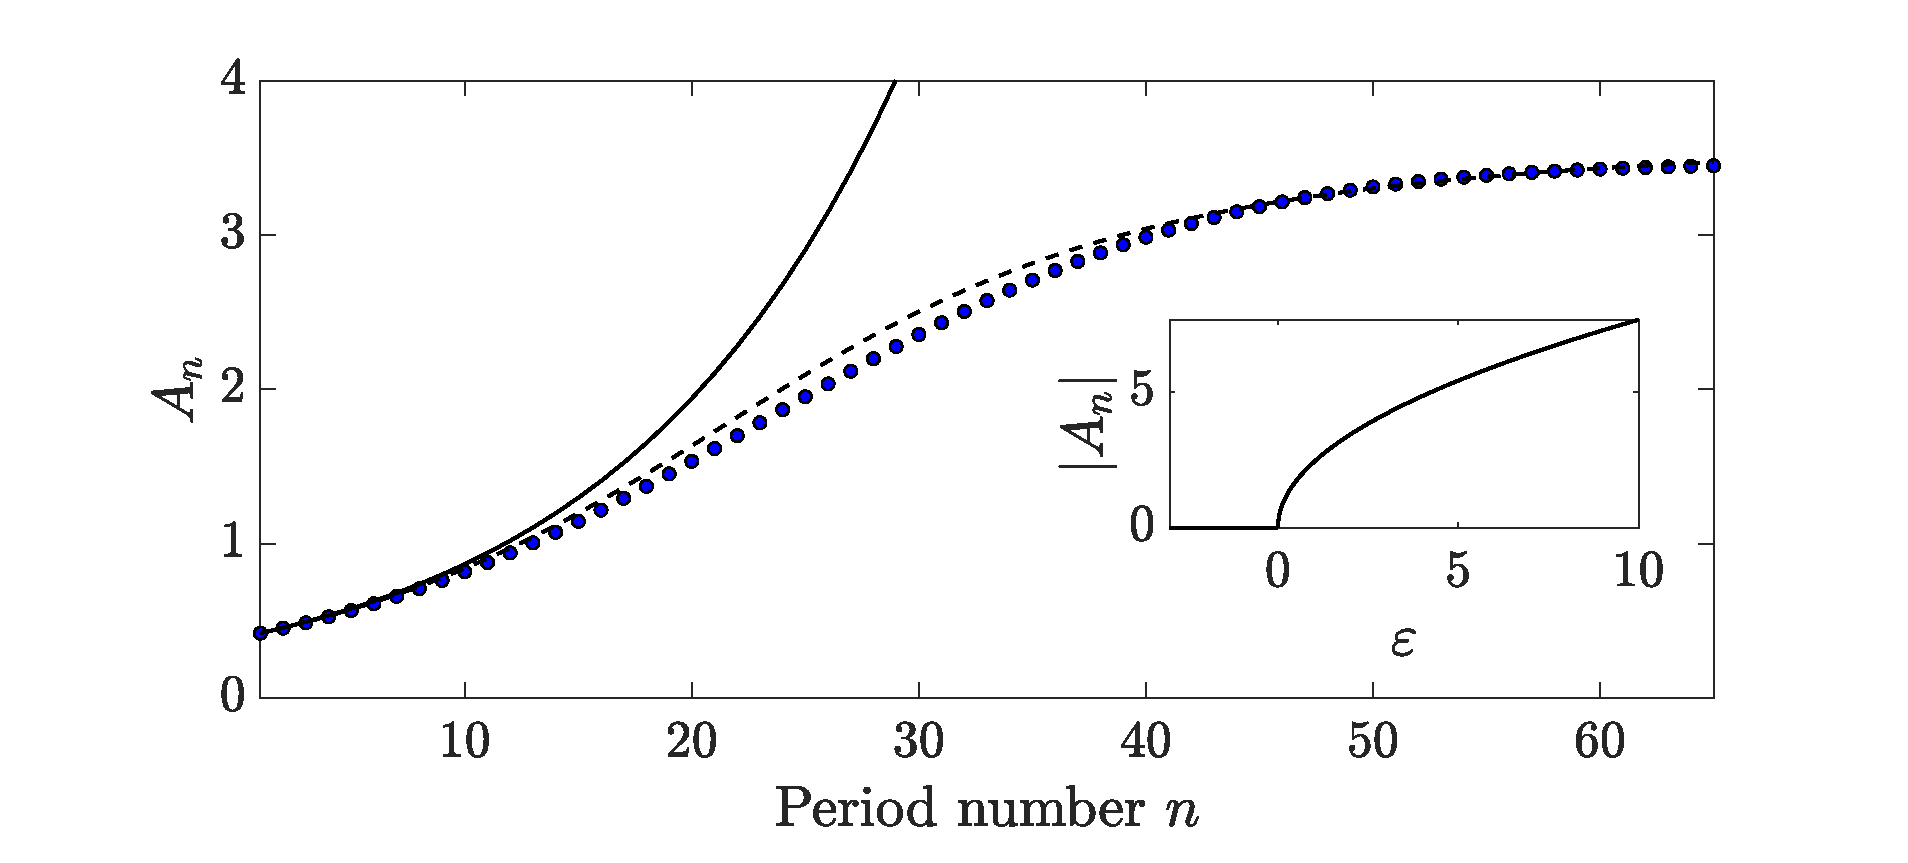
\includegraphics[width=0.7\textwidth]{./fig/AR4p5/Nlgrowth_Re420.eps}
  \caption{Nonlinear growth of the 2D perturbation to the wake near the secondary instability threshold for $\AR=4.5$ and $Re=420$. Top: the blue circles are the amplitude of $A_n$ evaluated from simulations of the full Navier--Stokes equations at $Re=420$. The solid line shows the prediction $A_{n+1} = \mu A_n$, while the dashed line shows the prediction $A_{n+1} = ( \mu + \alpha_1 A_n + \alpha_2 A_n^3 ) A_n$, with $\alpha_1 = -0.01114$ and $\alpha_2 = 0.000359$. The inset shows the bifurcation diagram.}
  \label{fig:ar4p5_nnl}
\end{figure}

The linear stability analysis presented in the previous section captures the onset of the instability but does not provide a description of the resulting asymmetric limit cycle. While linear theory is sufficient to determine the critical Reynolds number $Re_{c2}$, understanding the flow dynamics beyond the onset requires incorporating nonlinear effects.

Near a critical point, the wake dynamics can be approximated by a reduced-order discrete-time dynamical system, as proposed by \cite{henderson-barkley-1996} and \cite{henderson-1997}. To this end, we represent the full velocity field as
%
\begin{equation}
\bm{u}(\bm{x}, t) = U \bm{u}_0(\bm{x}, t) + A(t) \bm{u}_1(\bm{x}, t),
\end{equation}
%
where $||\bm{u}_0||=1$ and $||\bm{u}_1||=1$, $\bm{u}_0$ denotes the base flow, and $\bm{u}_1$ is the leading unstable Floquet mode with time-dependent amplitude $A(t)$. To reduce the problem to a discrete map, we sample the system at discrete times $t_n = t_0 + nT$, corresponding to successive base-flow periods. The flow field at each time step becomes
%
\begin{equation}
\bm{u}(\bm{x}, t_n) = U \bm{u}_0(\bm{x}, t_n) + A_n \bm{u}_1(\bm{x}, t_n),
\end{equation}
%
where $A_n \equiv A(t_n)$. Thus, the evolution of the flow is governed by the discrete-time dynamics of the amplitude $A_n$, while the evolution of $\bm{u}_1$ characterises the nonlinear distortion of the perturbation.

To classify the nature of the secondary instability, we adopt the normal form for a pitchfork bifurcation in a discrete-time dynamical system:
%
\begin{equation}
A_{n+1} = \left( \mu + \sum_{j=1}^{\infty} \alpha_j A_n^{2j} \right) A_n,
\end{equation}
%
where $\alpha_1$ is the Landau constant, and $\mu$ characterises the linear growth rate. The sign of $\alpha_1$ determines the nature of the bifurcation: if $\alpha_1<0$, the bifurcation is supercritical (soft); if $\alpha_1>0$, it is subcritical (hard) \citep{kuznetsov-1997}. In the supercritical case, the amplitude of the resulting nonlinear state can be approximated by retaining only the first two terms of the expansion. Introducing the reduced control parameter $\epsilon = (Re-Re_{c2})/Re_{c2}$, and writing $\mu = 1 + \mu' \epsilon$ (where $\mu'  = \partial \mu/\partial Re$), the equilibrium amplitude is given by
%
\begin{equation}
|A|^2 = - \frac{\mu' \epsilon}{\alpha_1}.
\end{equation}
%
It is worth emphasising that, owing to the two-dimensional and synchronous nature of the bifurcation, it is not possible to clearly separate the nonlinear evolution of the unstable mode from the distortion of the base flow. In contrast, such a separation would be feasible in the context of a weakly nonlinear stability analysis about the periodic limit cycle, where perturbations can be decomposed into distinct components associated with the leading mode and its higher-order interactions. In the present case, the bifurcating flow is time-periodic, and the instability develops synchronously with the base-cycle frequency. As a result, the nonlinear perturbation and the base flow evolve concurrently and interact nonlinearly in a coupled manner, preventing a clean modal decomposition. A formal weakly nonlinear analysis of the limit cycle, which could in principle isolate the contribution of the unstable Floquet mode and systematically capture its nonlinear saturation, lies beyond the scope of the present study.

To determine the nonlinear character of the secondary instability, we perform fully nonlinear simulations at $Re\approx Re_{c2}$, tracking the evolution of the perturbation field written as $\bm{u}_0 + \bm{u}_{nl}$, where $\bm{u}_{nl}$ represents the nonlinear correction. Simulations are initialised with $\bm{u}_{nl}(t_0) = \bm{u}_1(t_0)$, and the amplitude at each period is computed as
%
\begin{equation}
|A_n|^2 = \frac{1}{\Omega U_\infty^2} \int_\Omega |\bm{u}_{nl}(\bm{x},t_n)|^2 \mathrm{d} \Omega.
\end{equation}
%
The nonlinear coefficients $\alpha_j$ are then estimated from the evolution of $A_n$ over time.

Figure~\ref{fig:ar4p5_nnl} reports results for $\AR=4.5$ at $Re=420$ (corresponding to $\epsilon \approx 0.01$). Similar results are obtained for $\AR=4$. Starting from a small initial perturbation, the instability grows and saturates after approximately $\mathcal{O}(50)$ shedding periods. At this Reynolds number, the linear growth rate is $\mu = 1.083$. However, as the amplitude approaches saturation, the growth of $A_n$ slows and deviates from the exponential trend predicted by linear theory. Fitting the amplitude evolution yields a Landau coefficient $\alpha_1 \approx - 0.011<0$, indicating that the bifurcation is supercritical. This conclusion is consistent with the smooth transition observed in the $C_\ell-Re$ and $C_d-Re$ diagrams shown in figure~\ref{fig:Cl-Cd-AR4}.

\begin{figure}
  \centering
  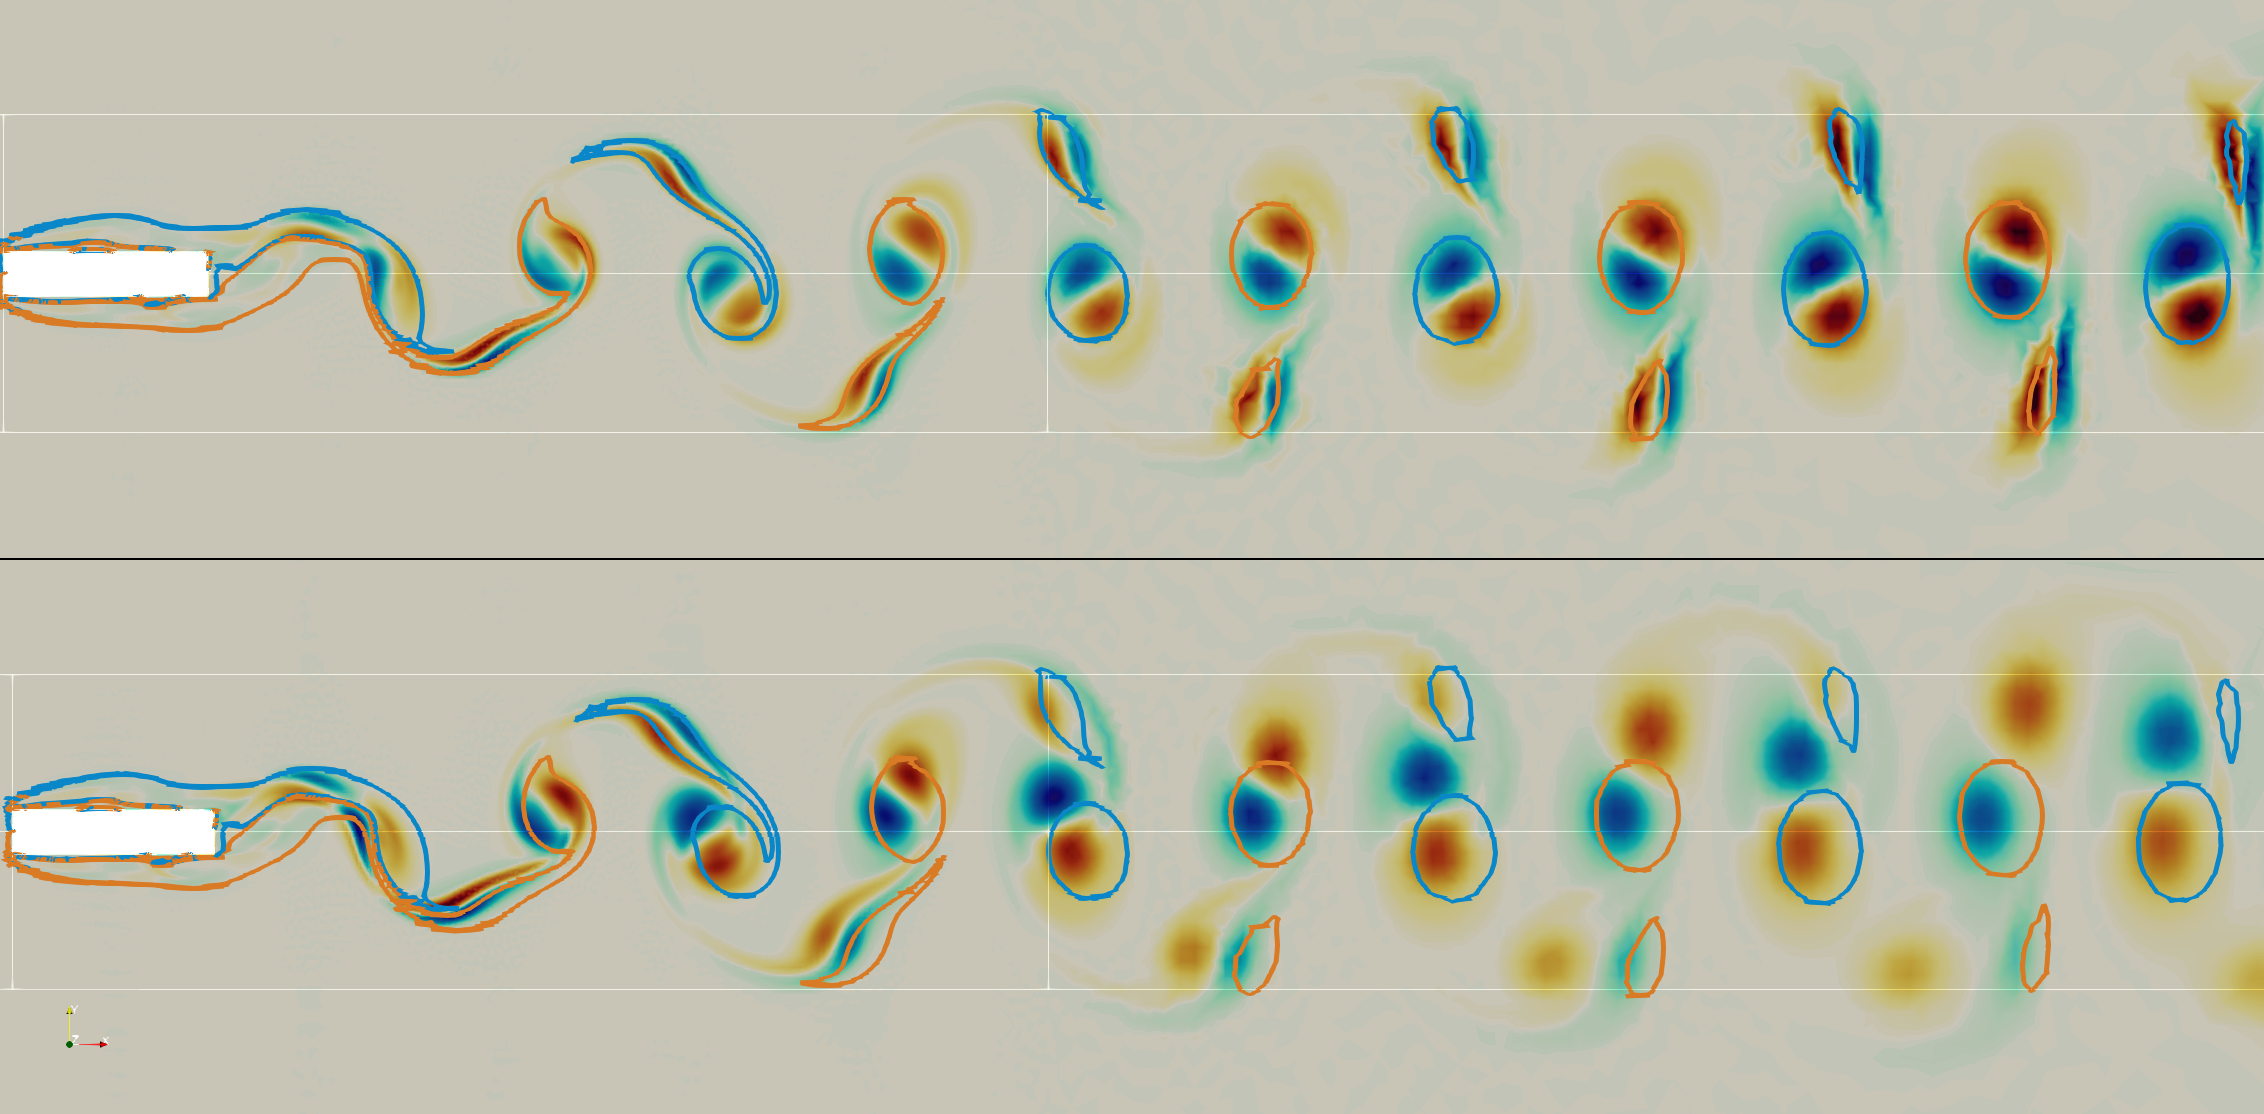
\includegraphics[width=0.9\textwidth]{./fig/AR4p5/nl_Re420.png}
  \caption{Perturbation field for $\AR=4.5$, $Re=420$ and $\beta=0$. Top: linear perturbation. Bottom: non linear perturbation.}
  \label{fig:pert-nl}
\end{figure}

Figure~\ref{fig:pert-nl} presents instantaneous snapshots of both the linear and nonlinear perturbation fields. As discussed previously, the linear perturbation is characterised by an array of dipolar structures aligned with the streamwise direction and centred on the monopolar vortices of the base flow. Immediately downstream of the TE, the nonlinear perturbation closely resembles the linear one, indicating that nonlinear effects remain negligible in the near wake.
%
However, as the flow progresses downstream, nonlinear interactions become increasingly significant. The structure of the nonlinear perturbation diverges from its linear counterpart, exhibiting a spatial reorganisation in the cross-stream direction. In particular, the dipolar vortices of the nonlinear perturbation are no longer centred on the base-flow monopoles. Instead, they spread laterally and arrange themselves such that the perturbation field locally counteracts the vorticity of the base flow. This leads to a partial cancellation of the base-flow vortices, effectively erasing the symmetry of the straight-wake configuration in the fully developed nonlinear flow.

\subsection{The 3D bifurcation}

\subsubsection{Linear stability analysis}

\begin{figure}
  \centering
  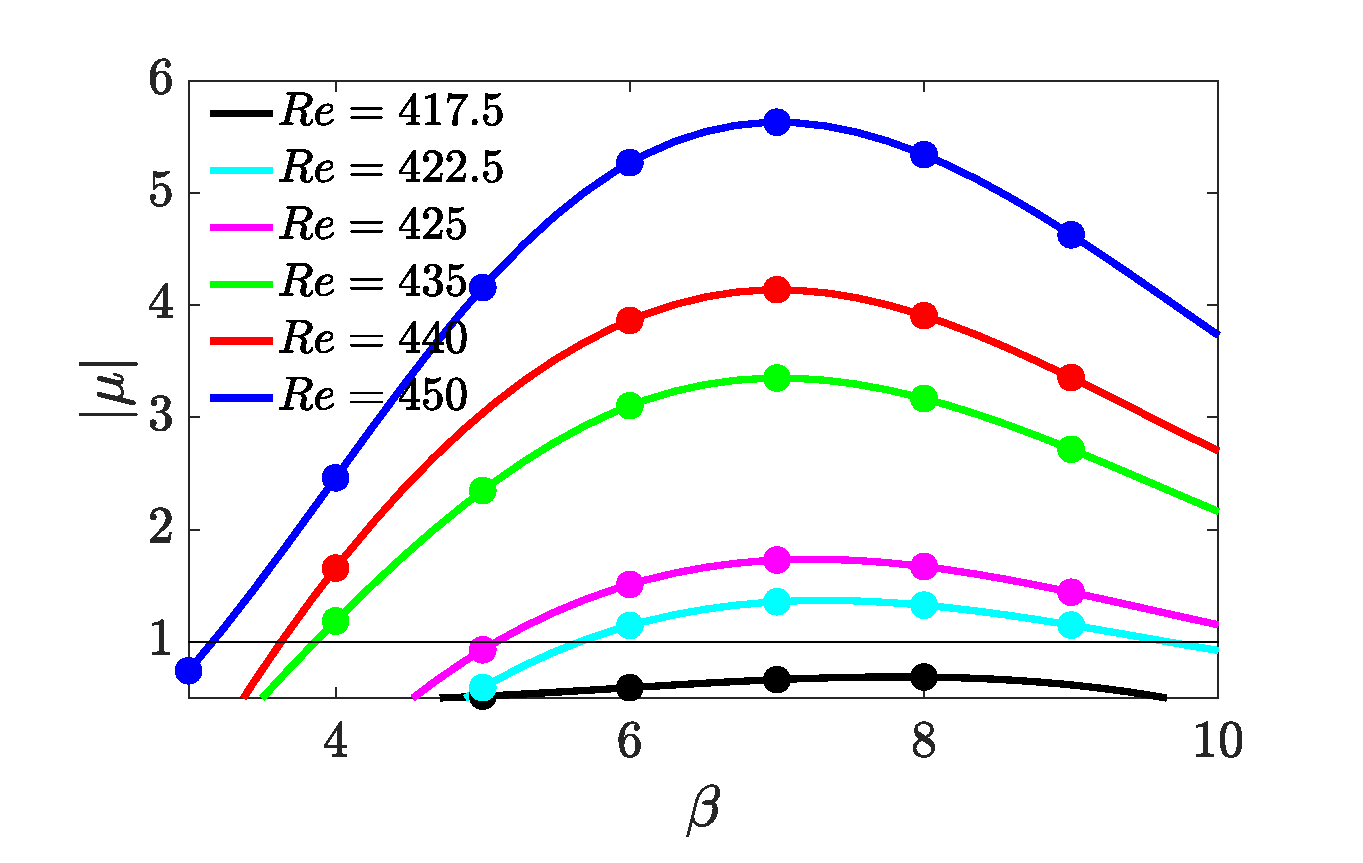
\includegraphics[width=0.49\textwidth]{./fig/AR4p5/multipliers_3D.eps}
  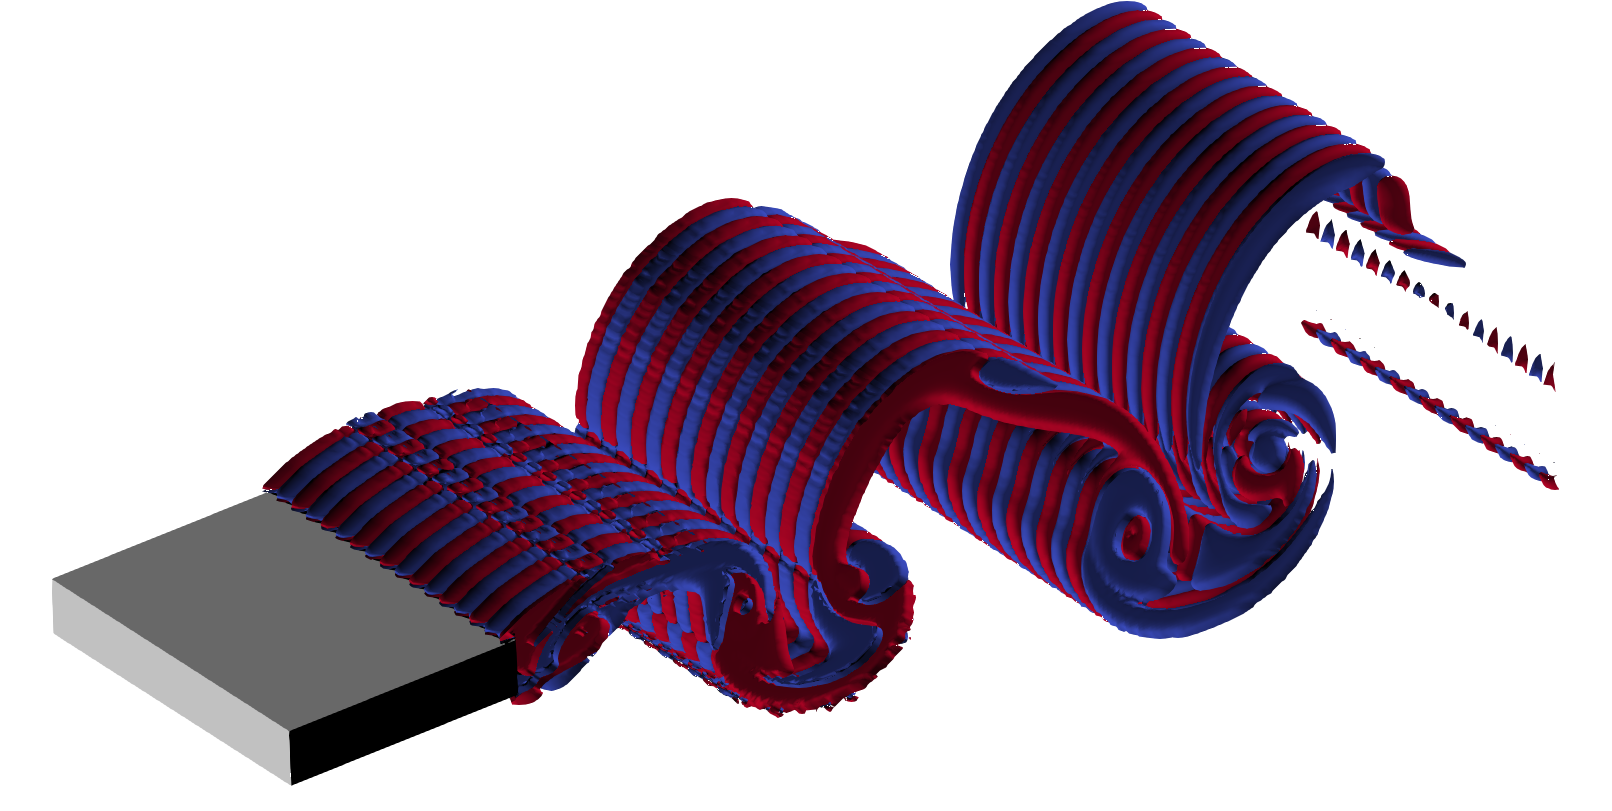
\includegraphics[trim={0 0 0 0},clip,width=0.7\textwidth]{./fig/AR4p5/Floqetmode_beta_8_Re450_AR4p5.png}  
  \caption{Three-dimensional instability for $\AR=4.5$. The flow becomes unstable to three-dimensiona perturbations once the was has bifurcated to a deflected configuration. The figure shows the dependence of the Floquet multilpiers on $Re$ and $\beta$. For all cases $\mu$ is real and negative, indicating a subharmonic bifurcation. Bottom: Imaginary part of the streamwise vorticity for $\AR=4.5$, $Re=450$ and $\beta=8$ associated with the unstable subharmonic multiplier. XX AGGIUNGIAMO QUA LA SENSITIVITA STRUTTURALE XX}
  \label{fig:mul-3d-ar4p5}
\end{figure}

As outlined in the previous section, for $Re \geq Re_{c2}$ the flow transitions to a new limit cycle characterised by a 2D asymmetric, deflected wake. This 2D deflected state, however, exhibits strong instability to 3D perturbations. We investigate its linear stability via Floquet analysis, focusing here on the case $\AR=4.5$ for conciseness, noting that qualitatively similar behaviour is observed for $\AR=4$.

Figure~\ref{fig:mul-3d-ar4p5} presents the leading Floquet multipliers as functions of the Reynolds number over the range $Re_{c2} \approx 417.5 \le Re \le 450$, and spanwise wavenumbers $3.5 \le \beta 10$. The onset of the first 3D instability occurs at $Re = Re_{c3} \approx 420$, associated with $\beta=7$. This indicates that the deflected two-dimensional wake remains stable only within a narrow interval beyond the bifurcation at $Re_{c2}$. For $Re>Re_{c3}$, a continuous band of unstable wavenumbers emerges, with the upper bound $\beta_{\max}$ exhibiting a weak dependence on $Re$. Notably, the growth rate of the instability increases rapidly with Reynolds number: the dominant multiplier attains $|\mu| \approx 2$ at $Re=425$ and $|\mu| \approx 9$ at $Re=450$.

The unstable Floquet multipliers are real and negative, indicating that the deflected wake is unstable to subharmonic 3D perturbations. As demonstrated by \cite{marques-lopez-blackburn-2004} and \cite{blackburn-etal-2005}, such subharmonic multipliers---real, negative, and with zero imaginary part---cannot arise in flows possessing spatio-temporal symmetry, as is typical of the low-$Re$ flow past symmetric 2D bodies. However, once this symmetry is broken, as in the present case, subharmonic instabilities can develop. Comparable behaviour has been documented in other asymmetric configurations, such as flow past a square cylinder at a non-zero incidence angle \citep{blackburn-sheard-2010}.

Figure~\ref{fig:3dmode-ar4p5}(a) depicts the spatial structure of the real part of the streamwise vorticity associated with the unstable Floquet mode at $Re=450$ and $\beta=8$. The perturbation is concentrated near the vortex cores of the base flow, a characteristic feature of wake instabilities in bluff-body flows \citep[e.g.,][]{thompson-leweke-williamson-2001, chaurasia-thompson-2011}. Notably, the disturbance is highly localised within the wake region, exhibiting negligible amplitude along the lateral sides of the cylinder. This distinguishes the present mode from the QS instability discussed by \cite{chiarini-quadrio-auteri-2022d} (see also the following section), which is driven by the LE vortices. Instead, the current mode arises as an intrinsic unstable mode of the wake itself. Its spatial symmetry aligns with its subharmonic character: the sign of the streamwise vorticity alternates between successive periods, consistent with a Floquet multiplier satisfying $\Re(\mu)<0$ and $\Im(\mu)=0$.

\begin{figure}
  \centering
  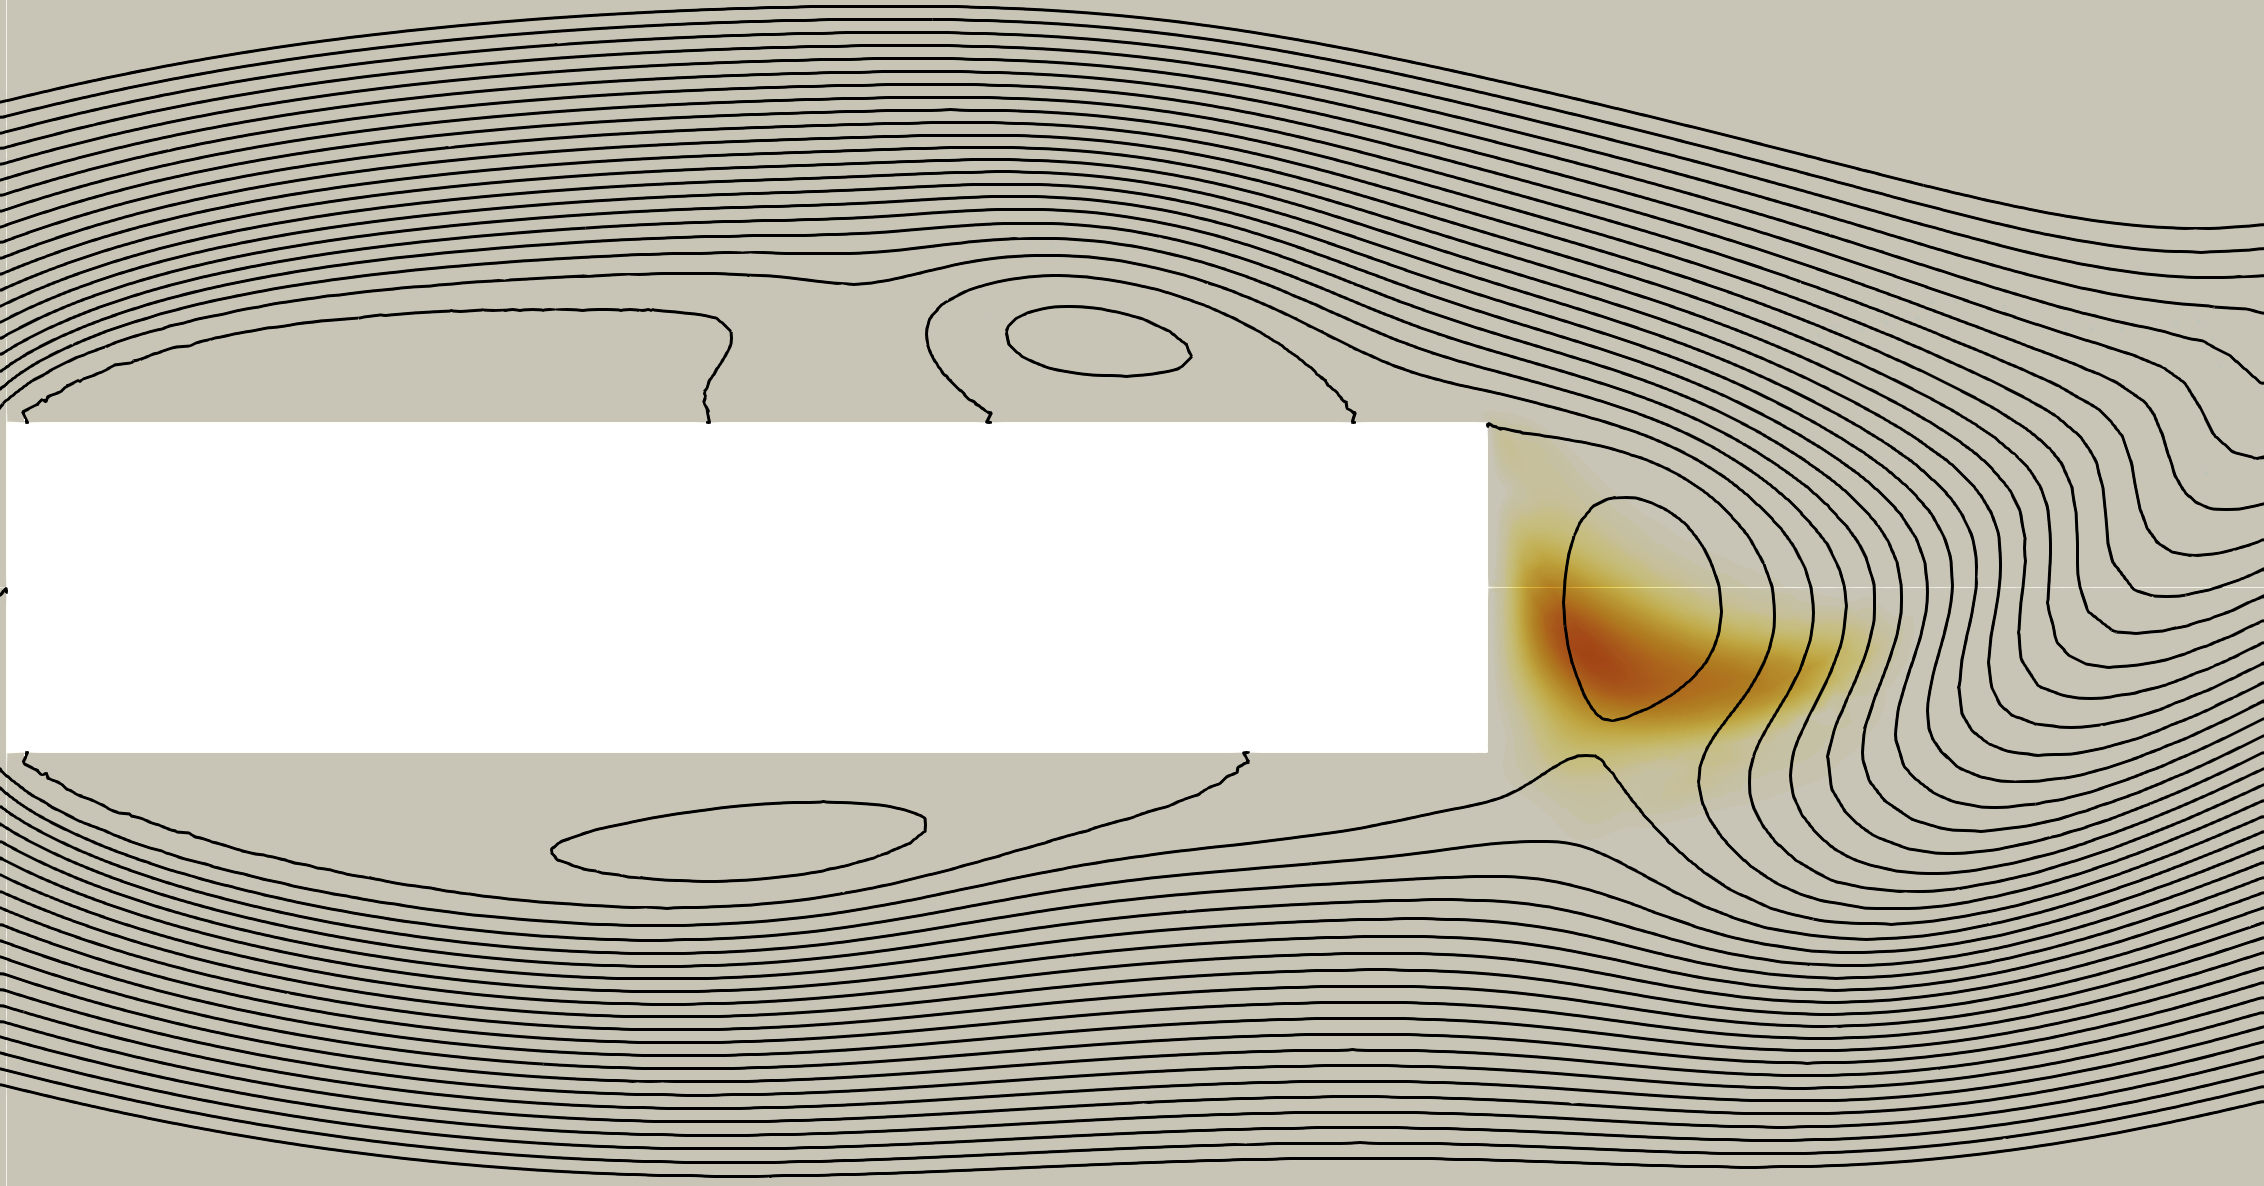
\includegraphics[width=0.49\textwidth]{./fig/AR4p5/sens3D_25.png}
  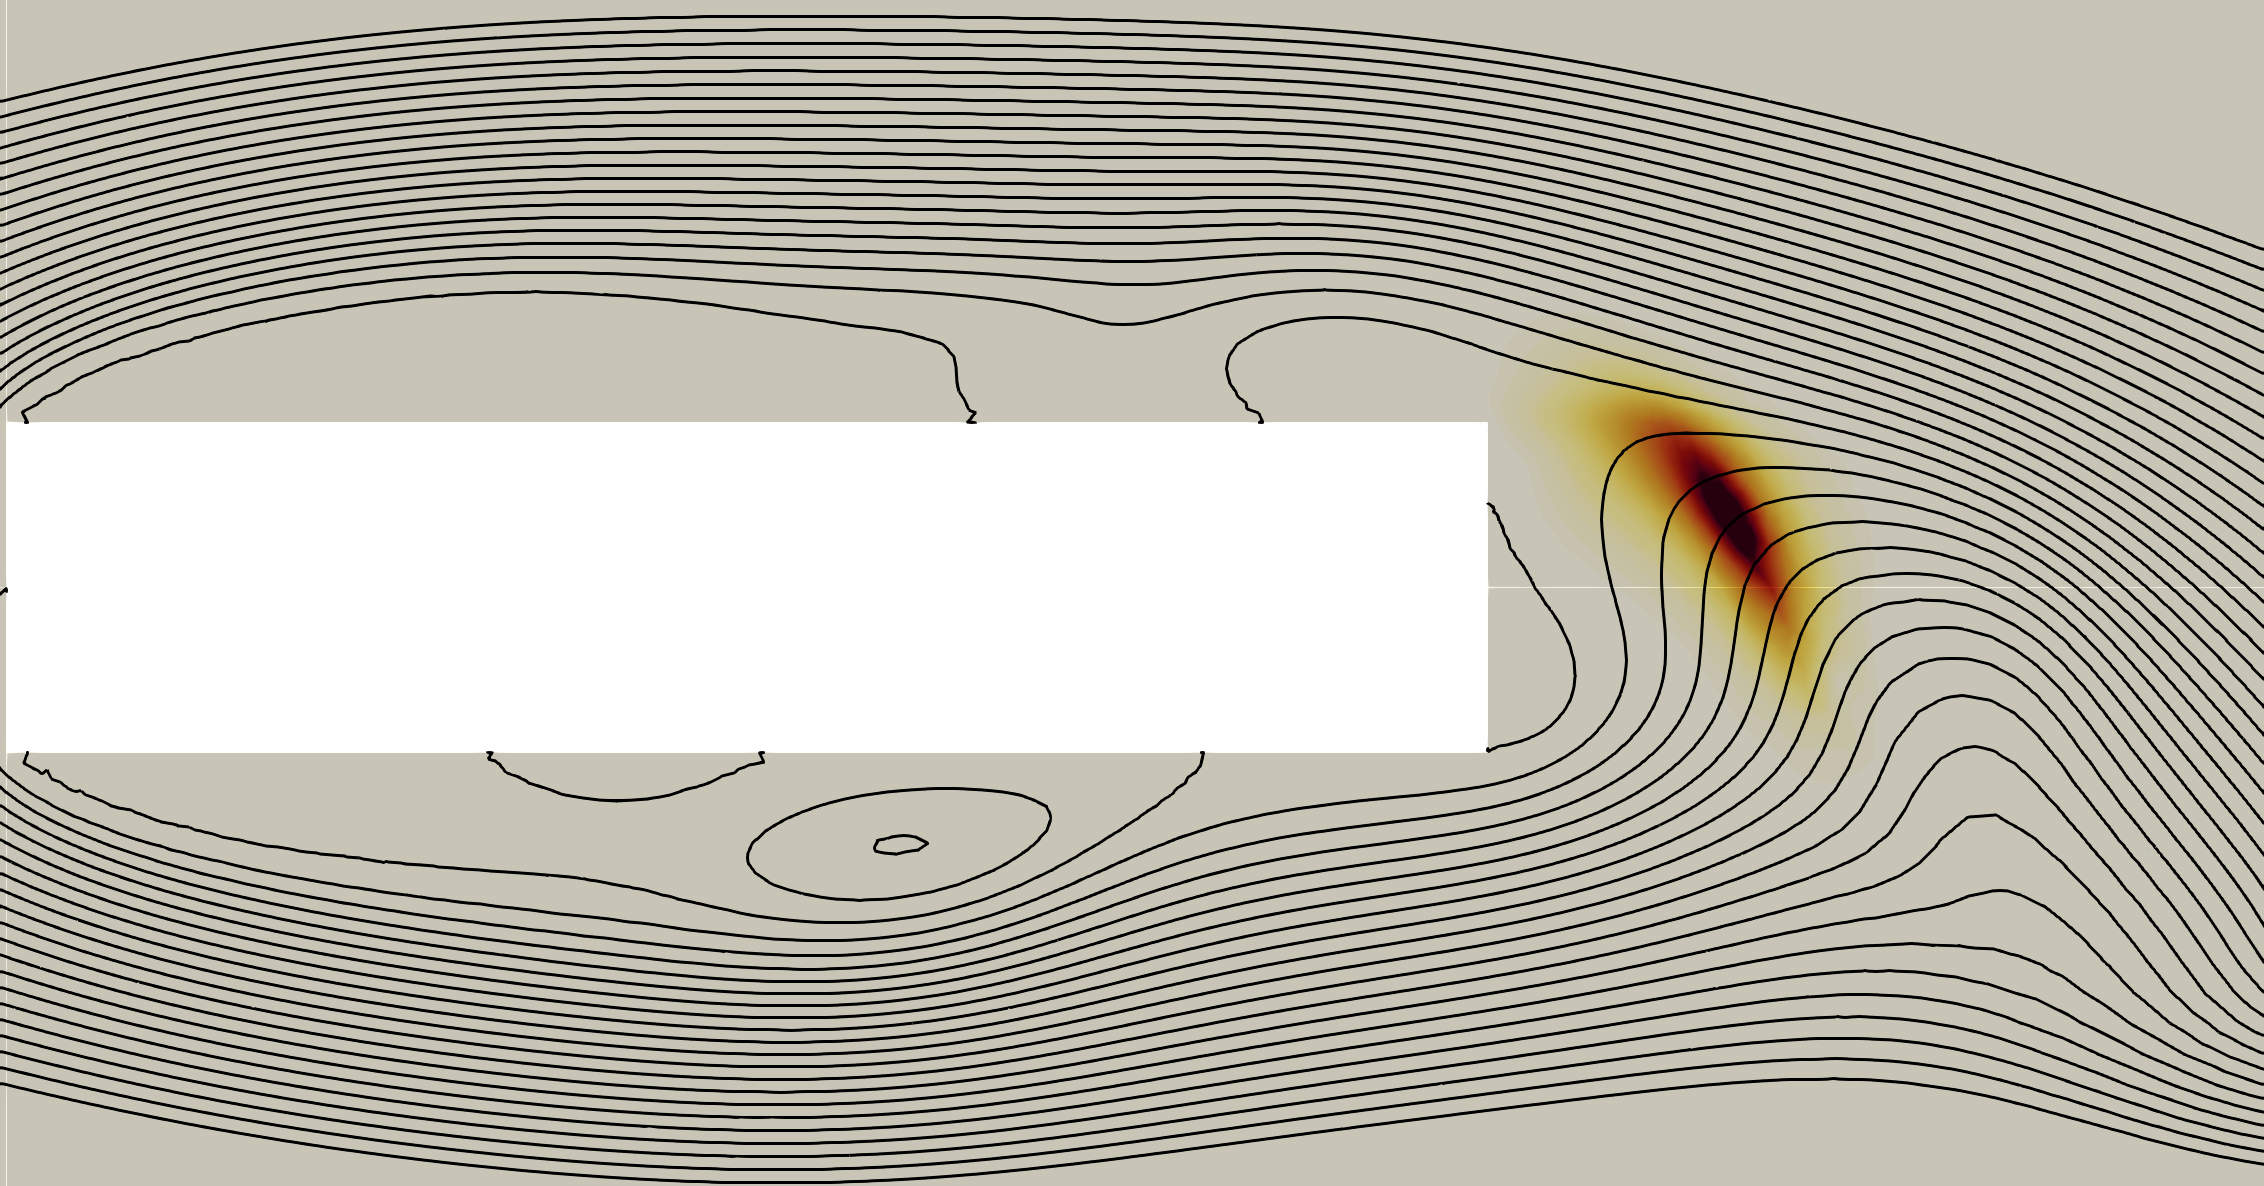
\includegraphics[width=0.49\textwidth]{./fig/AR4p5/sens3D_50.png}
  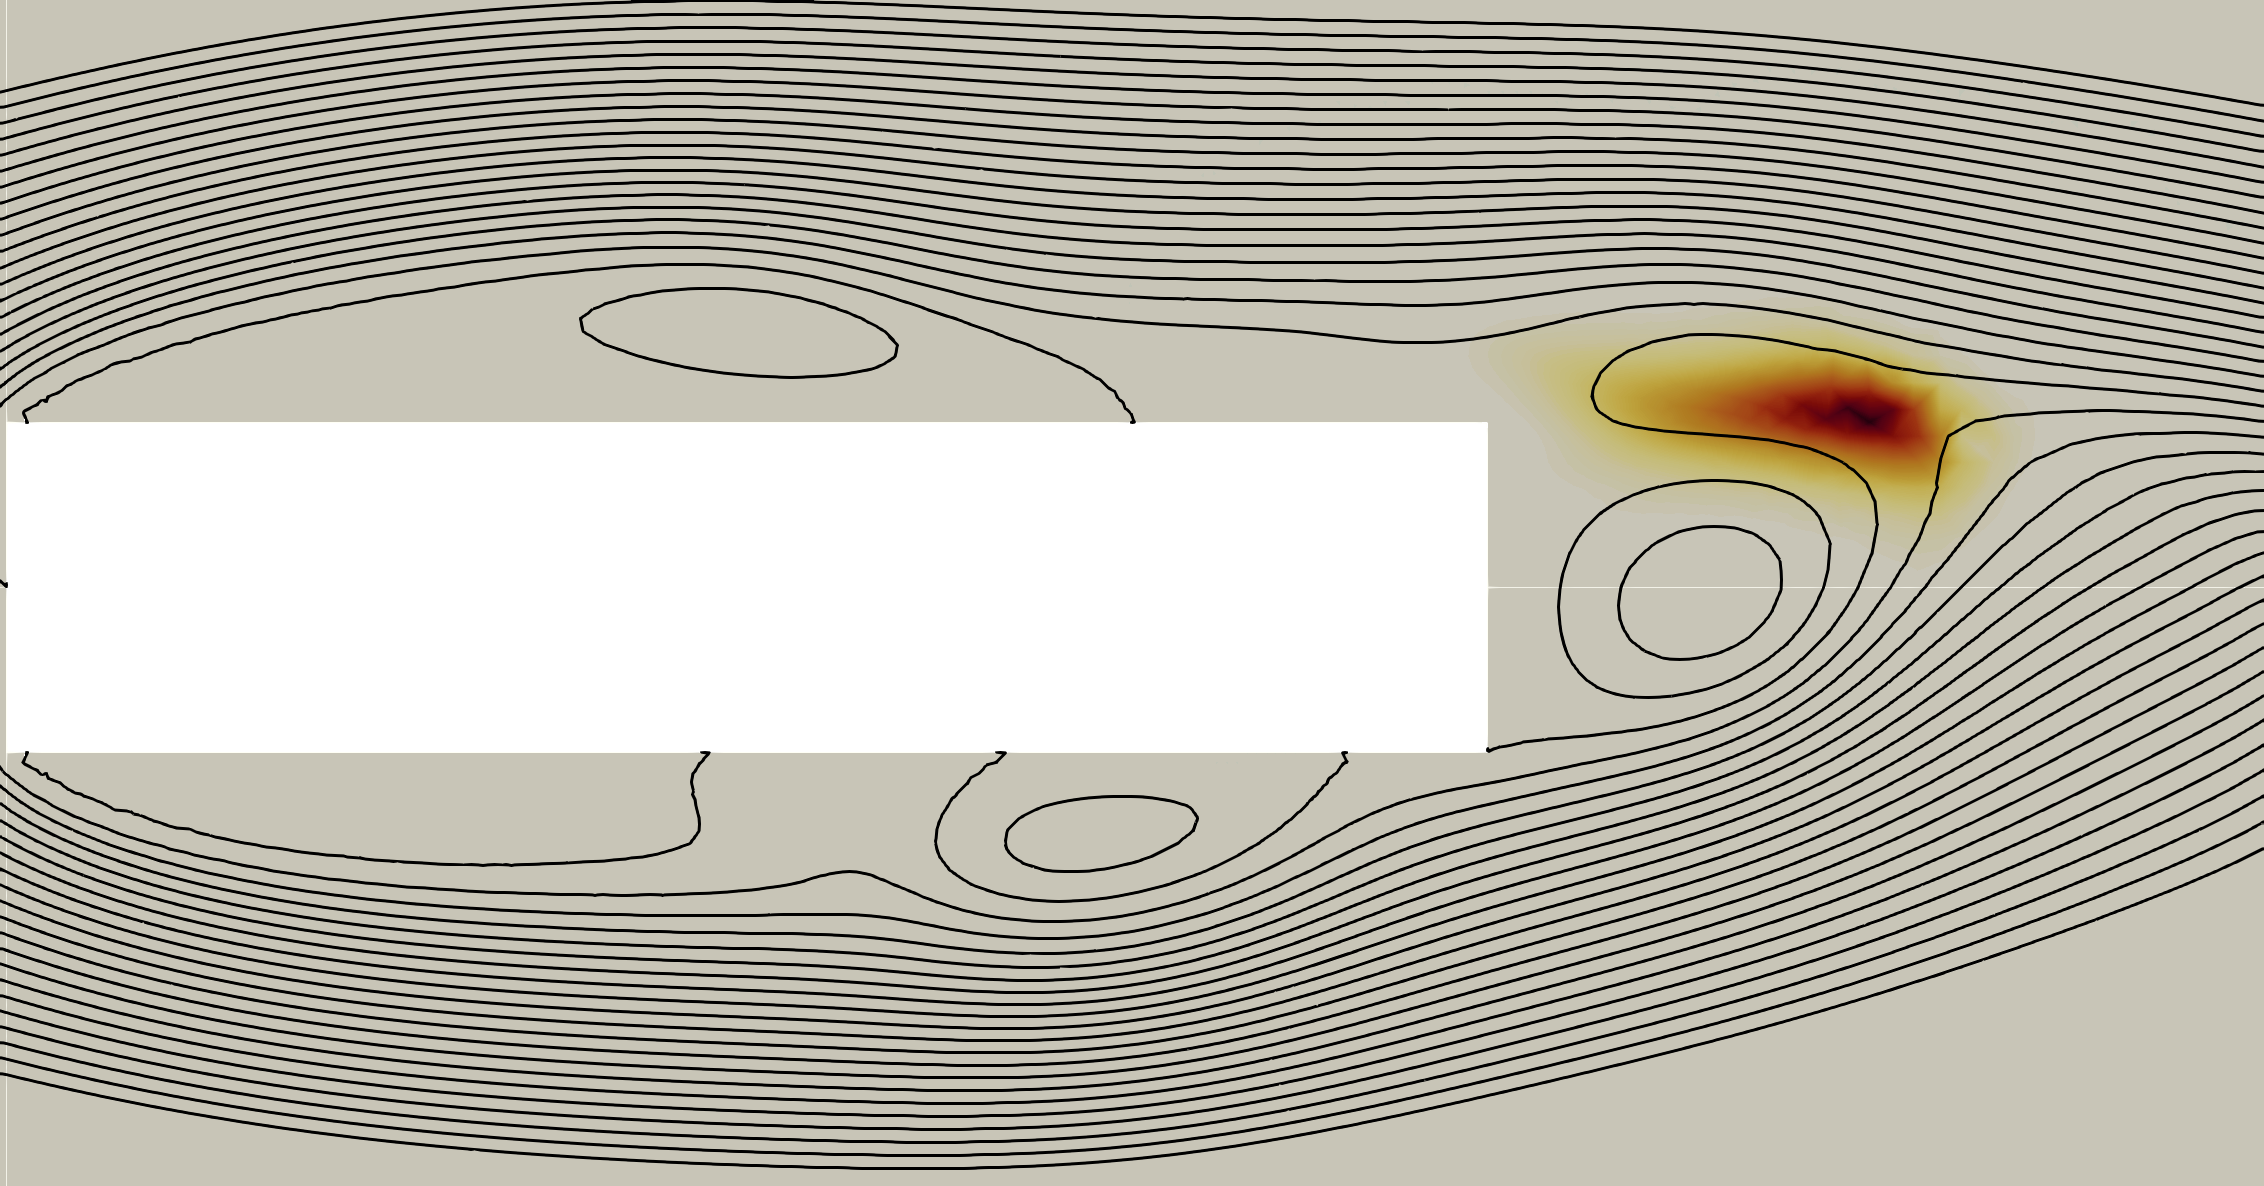
\includegraphics[width=0.49\textwidth]{./fig/AR4p5/sens3D_75.png}
  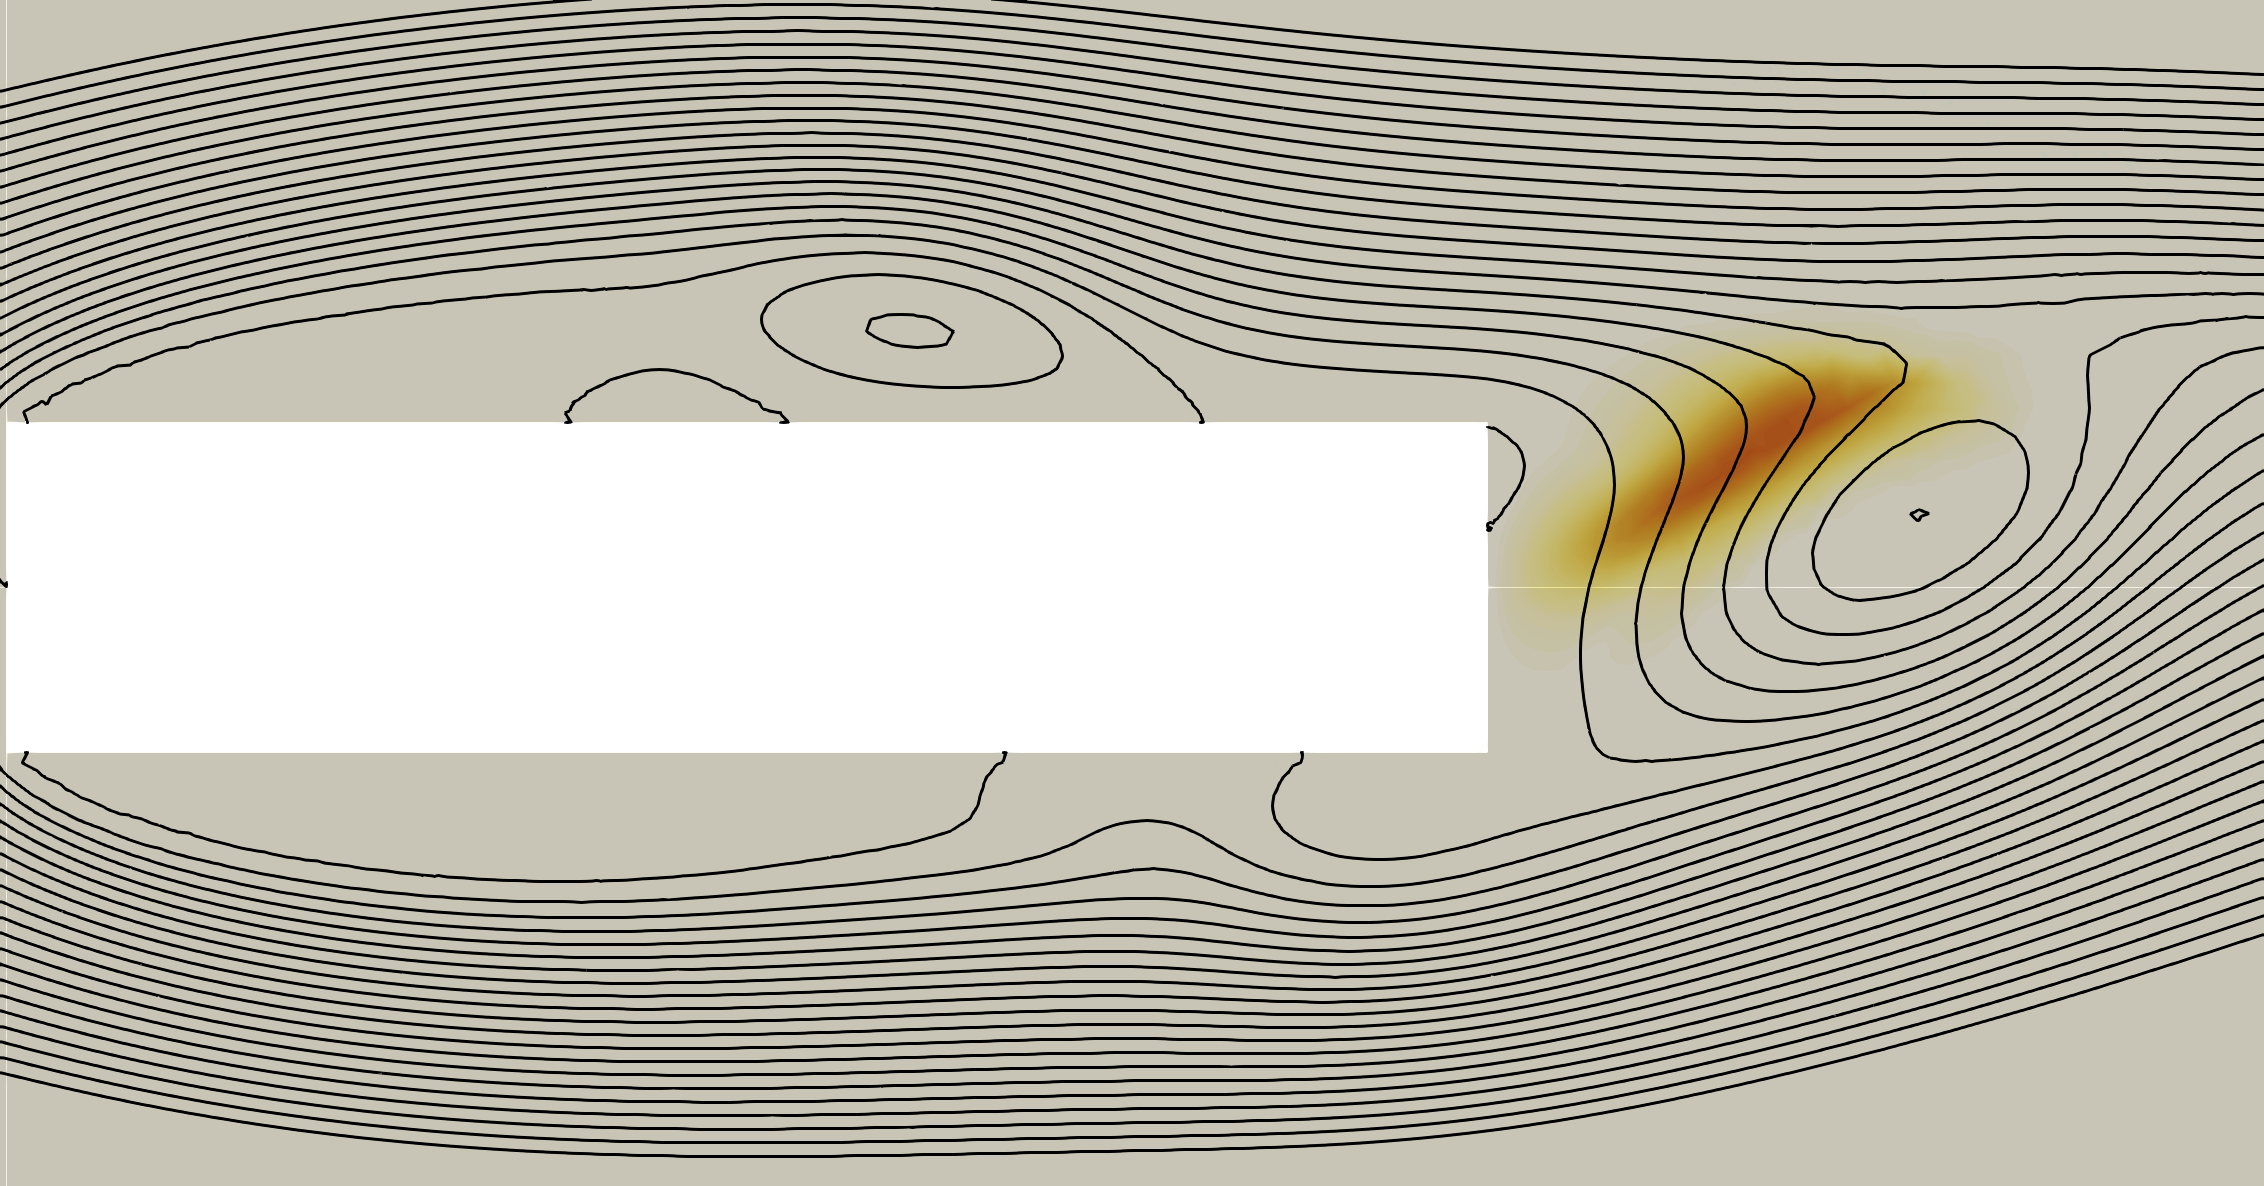
\includegraphics[width=0.49\textwidth]{./fig/AR4p5/sens3D_100.png}
  \caption{Structural sensitivity for $\AR=4.5$ and $\beta=8$ and $Re=450$ related to the 3D unstable mode. The four panels refer to four distinct time instants taken equispaced within the shedding period.}
  \label{fig:ss3d}
\end{figure}

To further characterise this 3D instability and identify the associated wavemaker region, we compute the spectral norm of the instantaneous structural sensitivity tensor $I$, following the formulation of \cite{giannetti-camarri-luchini-2010}. This quantity is defined as
%
\begin{equation}
I(x, y, \beta, t) = \frac{ \hat{\bm{u}}^\dagger(x, y, \beta, t), \hat{\bm{u}}(x, y, \beta, t) }{ \int_t^{t+T} \int_{\Omega} \hat{\bm{u}}^\dagger \cdot \hat{\bm{u}}, \mathrm{d}\Omega, \mathrm{d}t },
\end{equation}
%
where $\hat{\bm{u}}$ and $\hat{\bm{u}}^\dagger$ denote the direct and adjoint Floquet modes, respectively. The direct mode highlights regions of largest perturbation growth, while the adjoint mode represents the receptivity of the flow to external disturbances. Their pointwise product---the structural sensitivity $I$---thus localises the regions of strongest feedback between amplification and receptivity, identifying the so-called wavemaker region \citep{monkewitz-huerre-chomaz-1993}.

As a product of time-periodic direct and adjoint modes, the structural sensitivity inherits the periodicity of the base flow, satisfying $I(x,y,\beta,t) = I (x,y,\beta,t+T)$. The spectral norm $||I||$ is found to be negligible throughout most of the domain, except in a confined region just downstream of the TE, confirming that the instability is localised within the wake and is not driven by upstream LE vortex dynamics.

The maximum of $I$ remains localised near the TE vortex throughout the entire shedding cycle, indicating that the wavemaker is tightly coupled to the unsteady vortex dynamics in this region. Notably, at phase instants $t/T=0.25$ and $t/T=0.75$, the peak sensitivity coincides with the hyperbolic stagnation point formed just downstream of the TE. At $t/T=0.5$ and $t/T=1$, the sensitivity maximum shifts to the region of maximum streamline curvature within the vortex structure. This phase-dependent localisation confirms that the triggering and feedback mechanisms responsible for the instability are embedded in the dynamics of the TE vortex interaction and are modulated periodically in time.

\subsubsection{Non linear simulations}

\begin{figure}
  \centering
  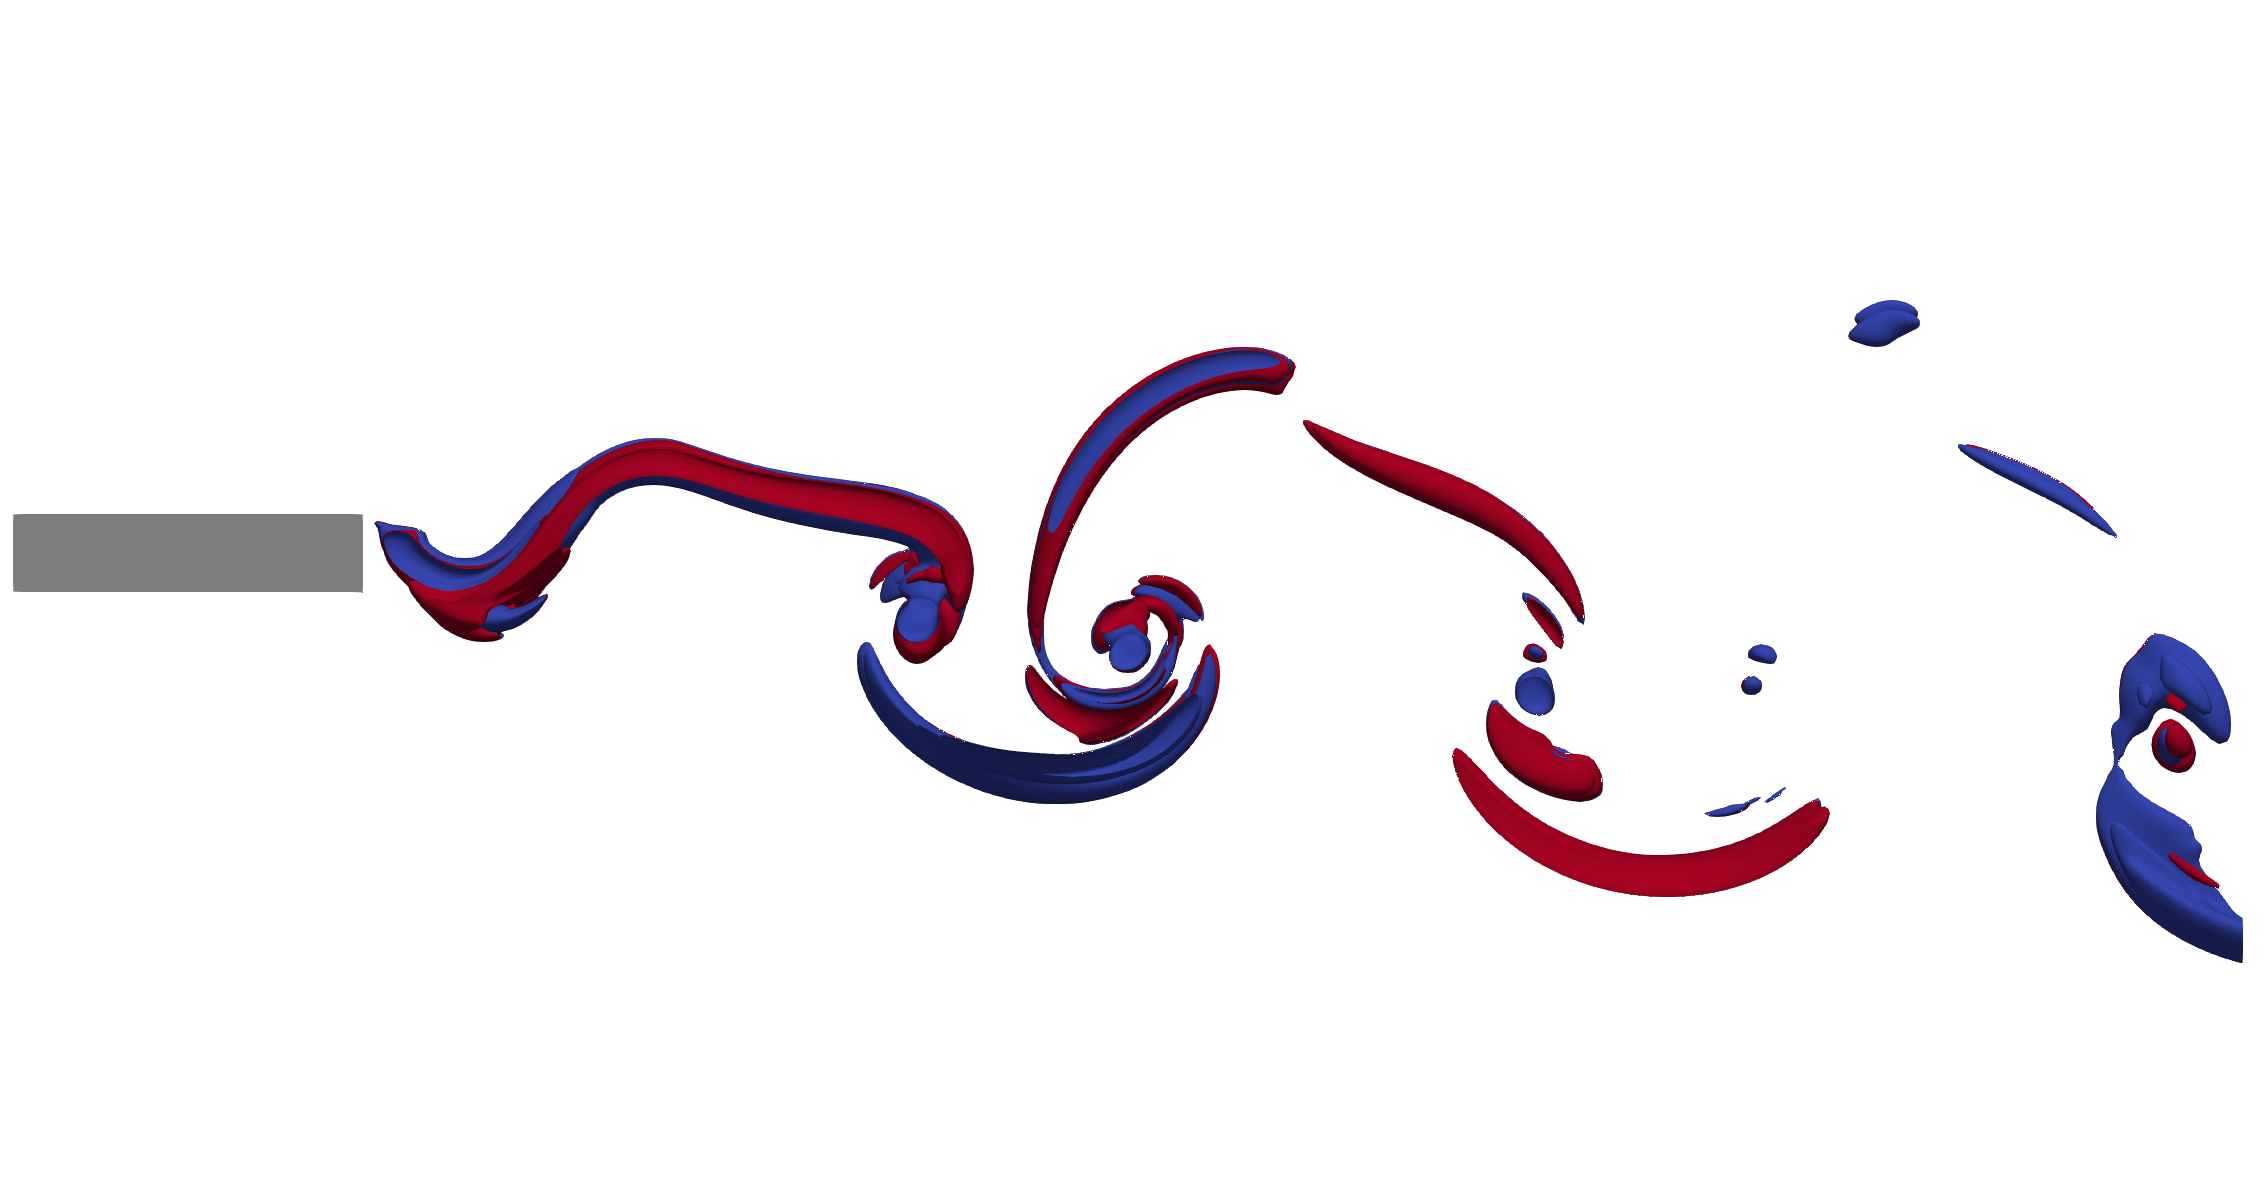
\includegraphics[trim={0 250 0 200},clip,width=0.49\textwidth]{./fig/AR4p5/omegax_Re425_2D.png}
  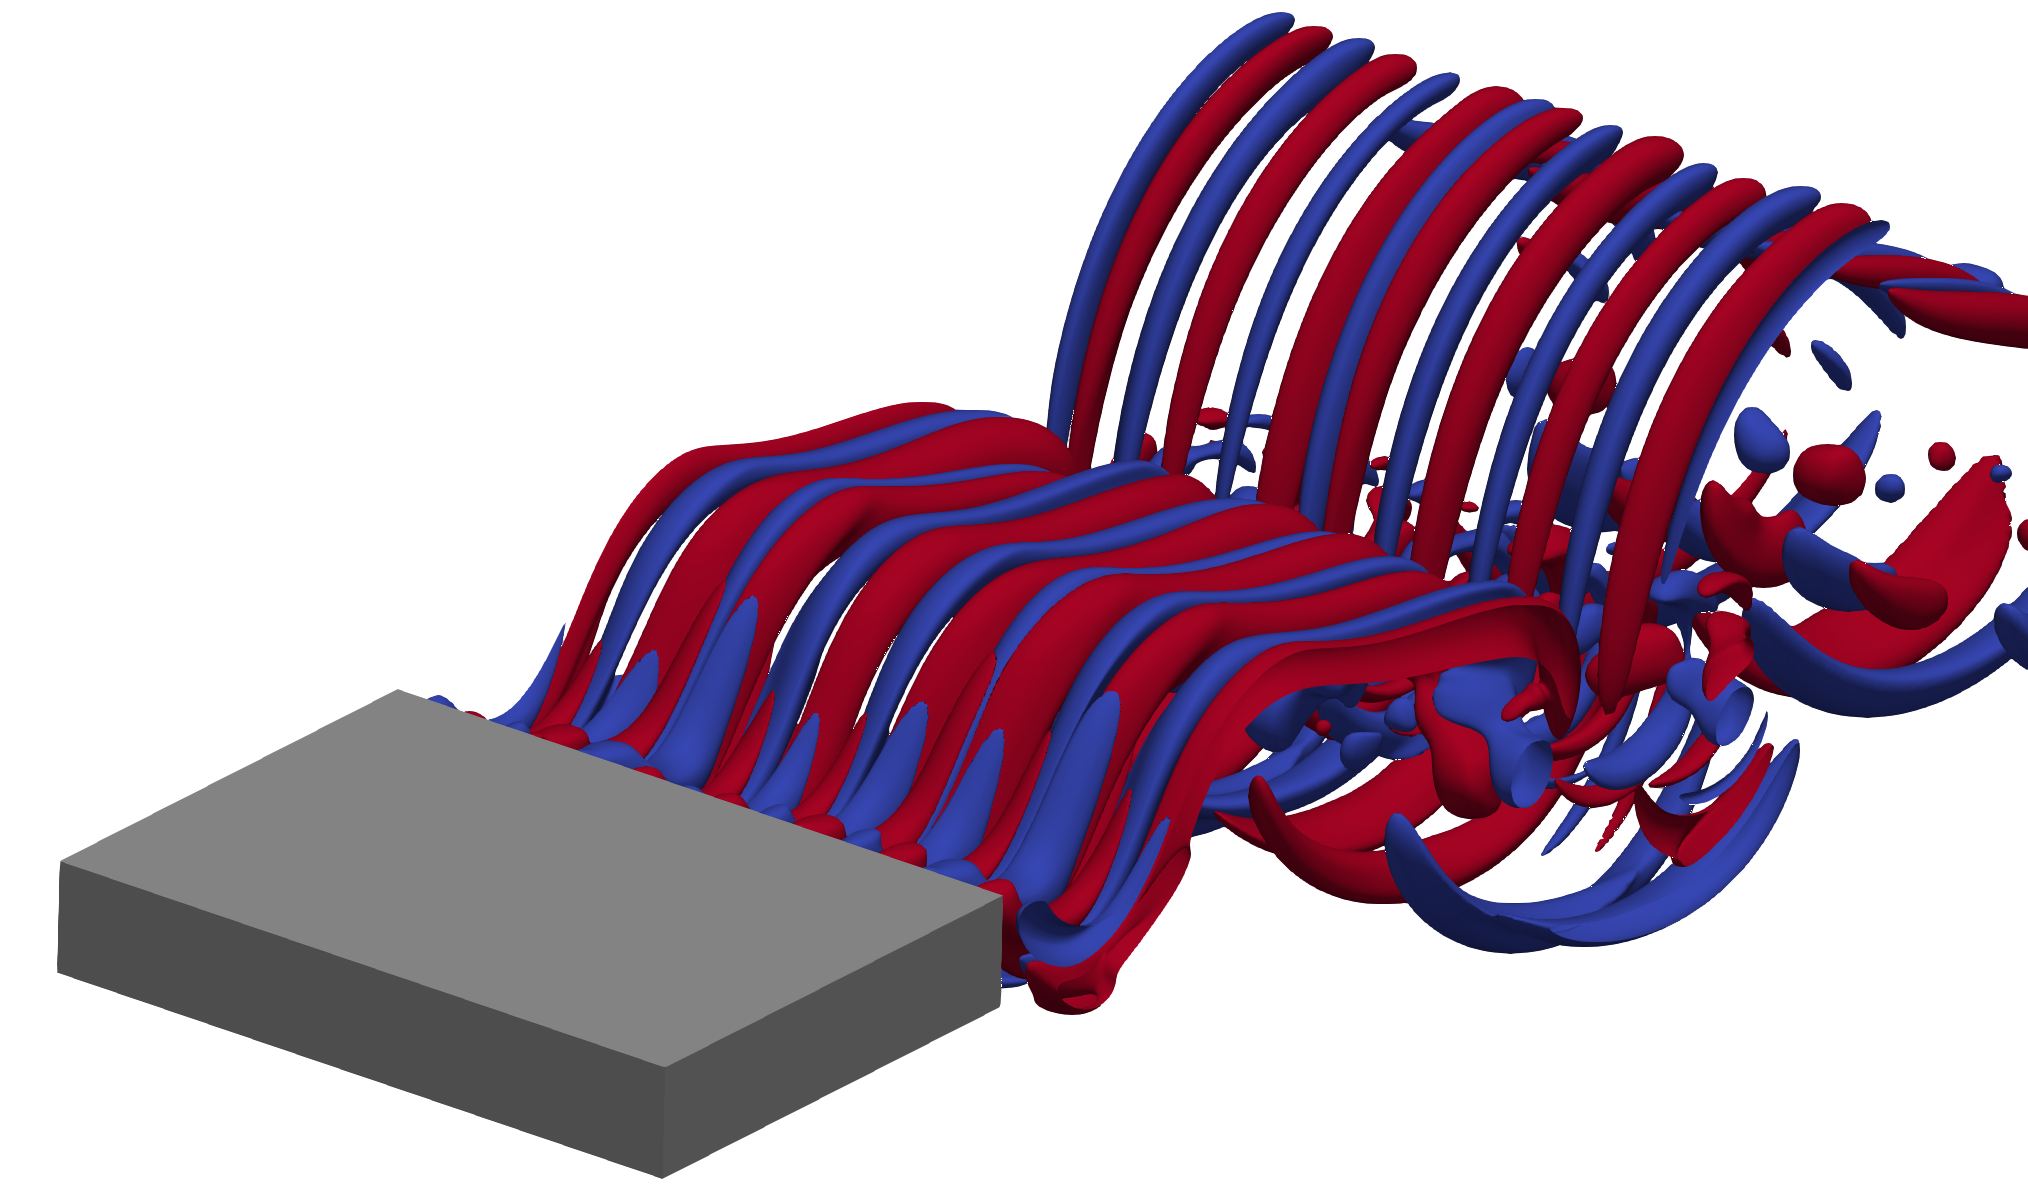
\includegraphics[trim={10 0 10 0},clip,width=0.49\textwidth]{./fig/AR4p5/omegax_Re425_3D.png} 
  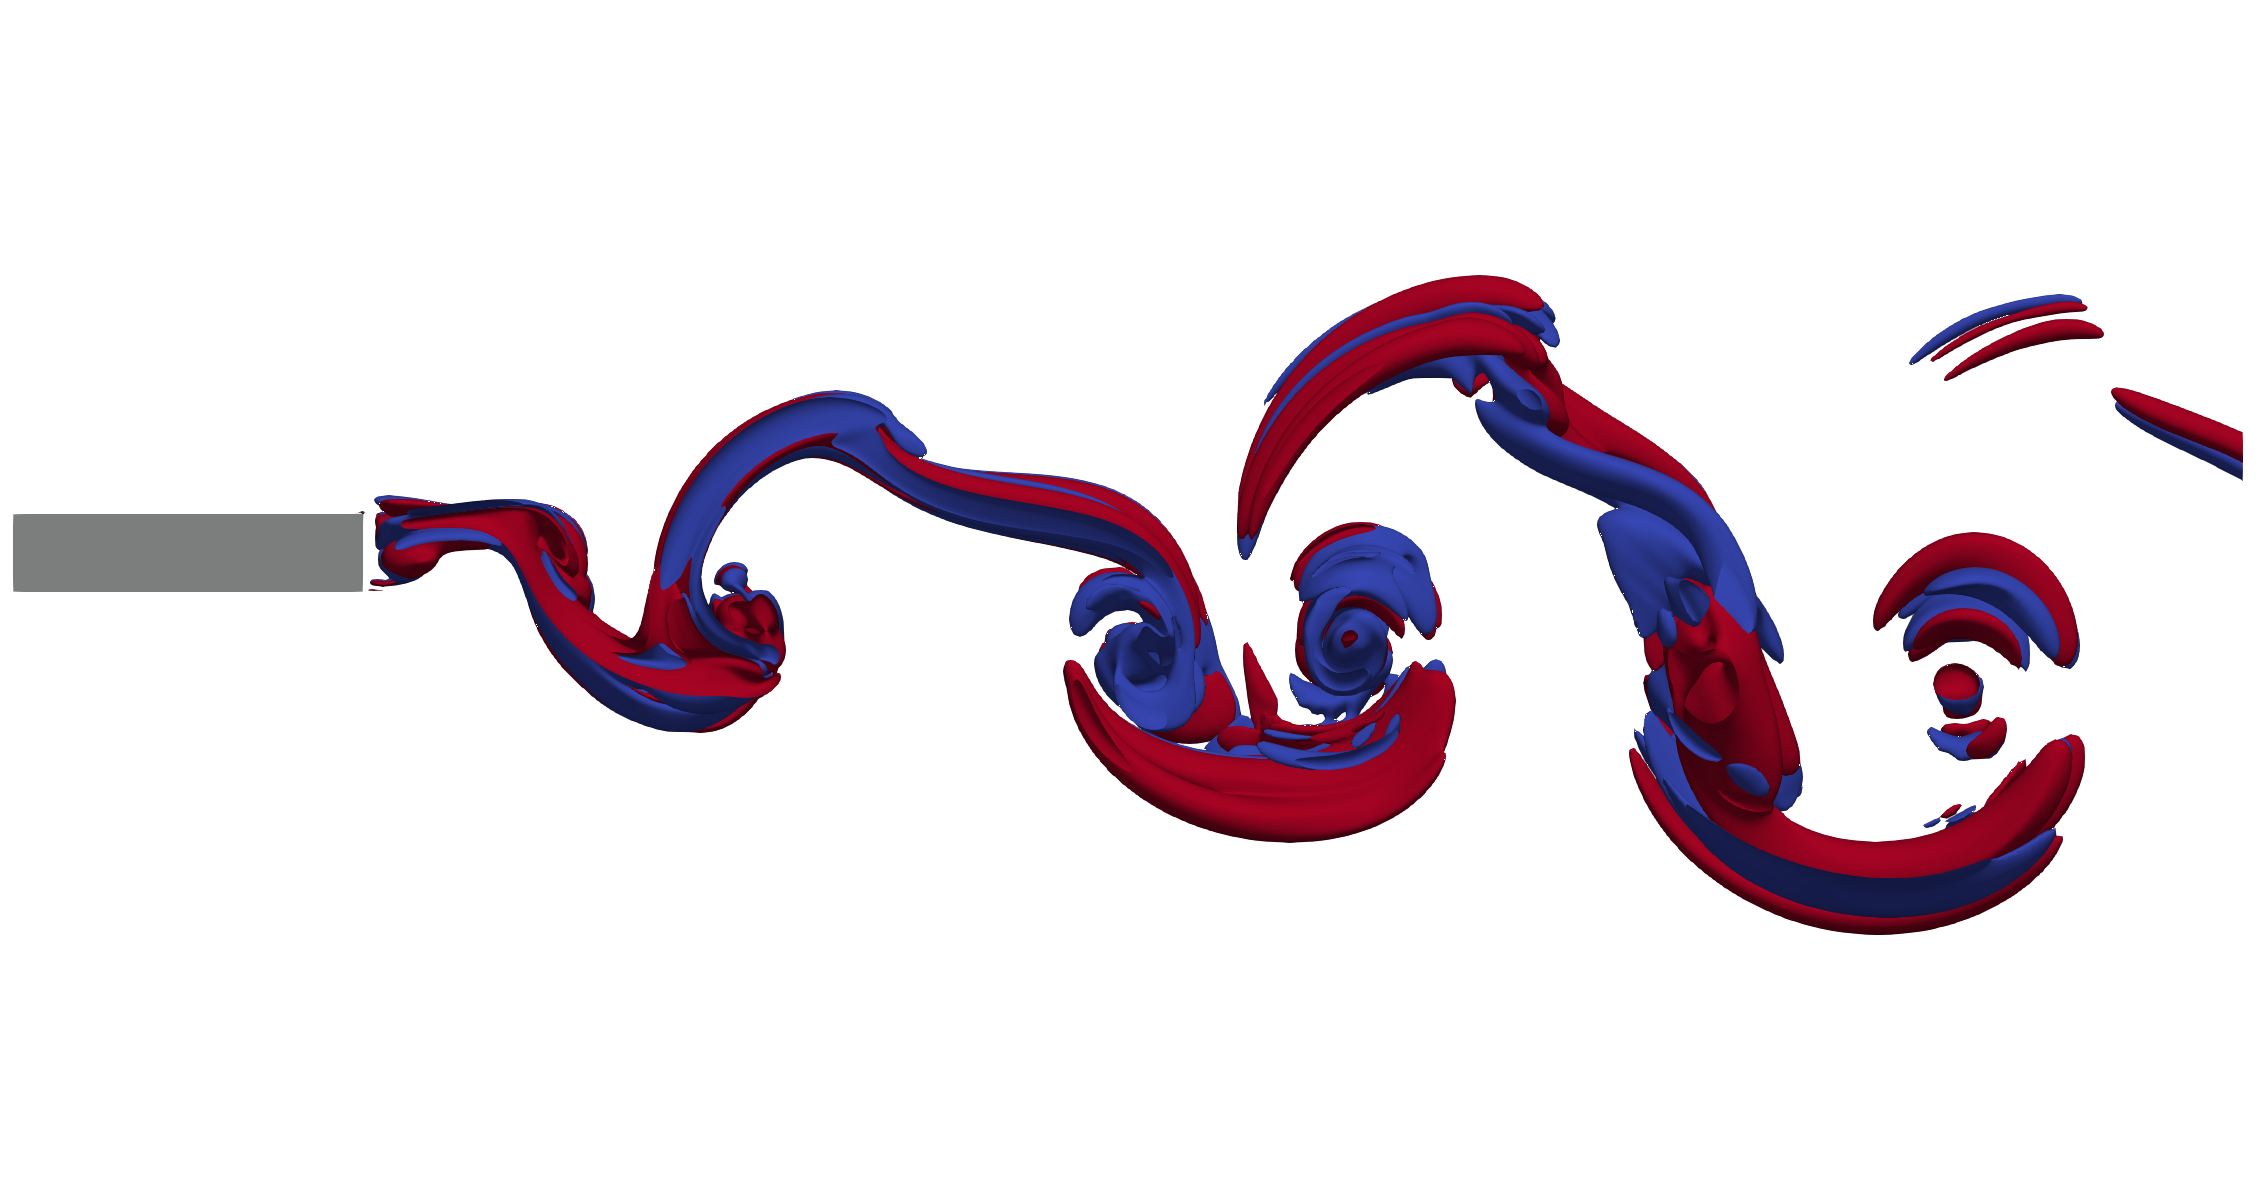
\includegraphics[trim={0 250 0 200},clip,width=0.49\textwidth]{./fig/AR4p5/omegax_Re450_2D.png}
  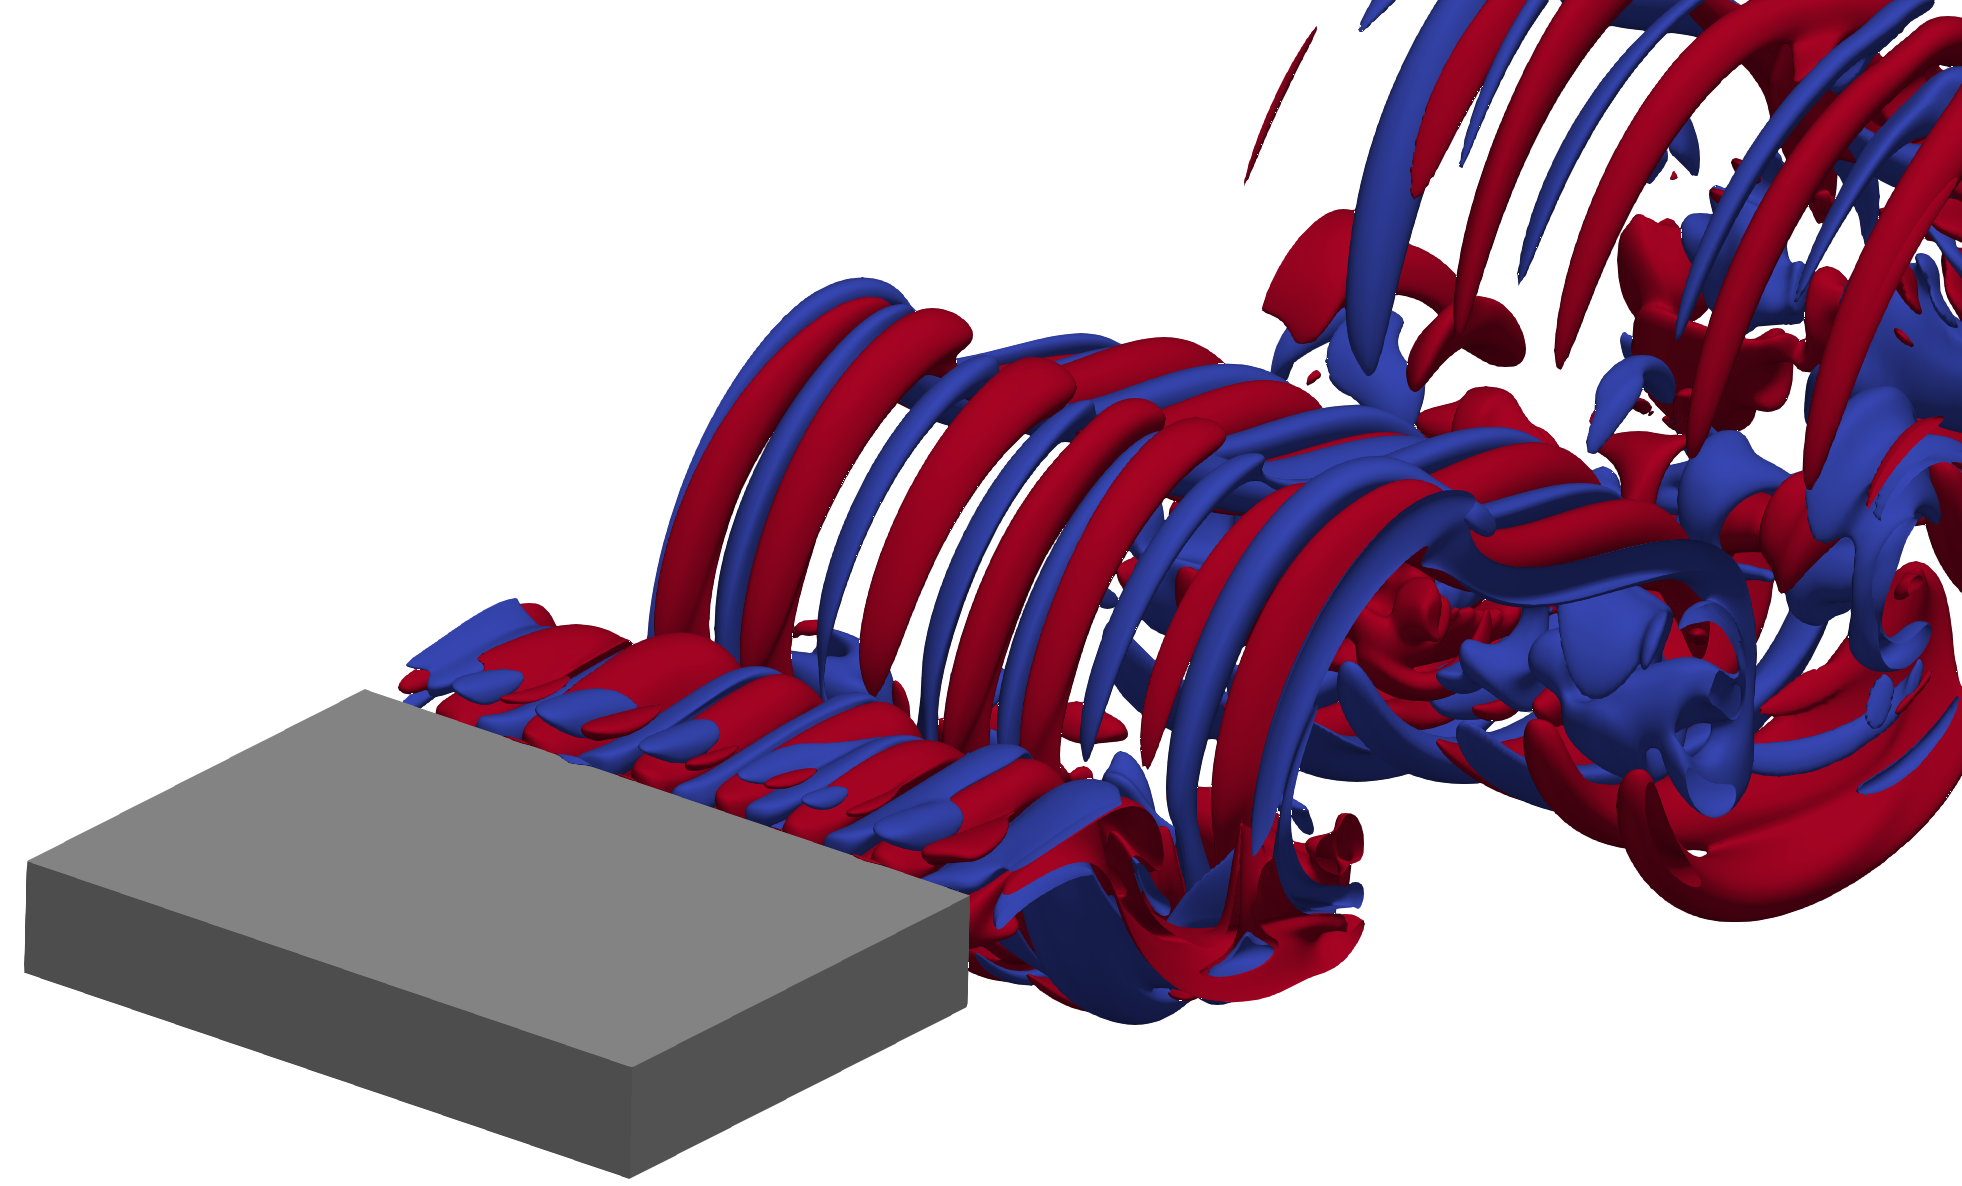
\includegraphics[trim={10 0 10 0},clip,width=0.49\textwidth]{./fig/AR4p5/omegax_Re450_3D.png} 
  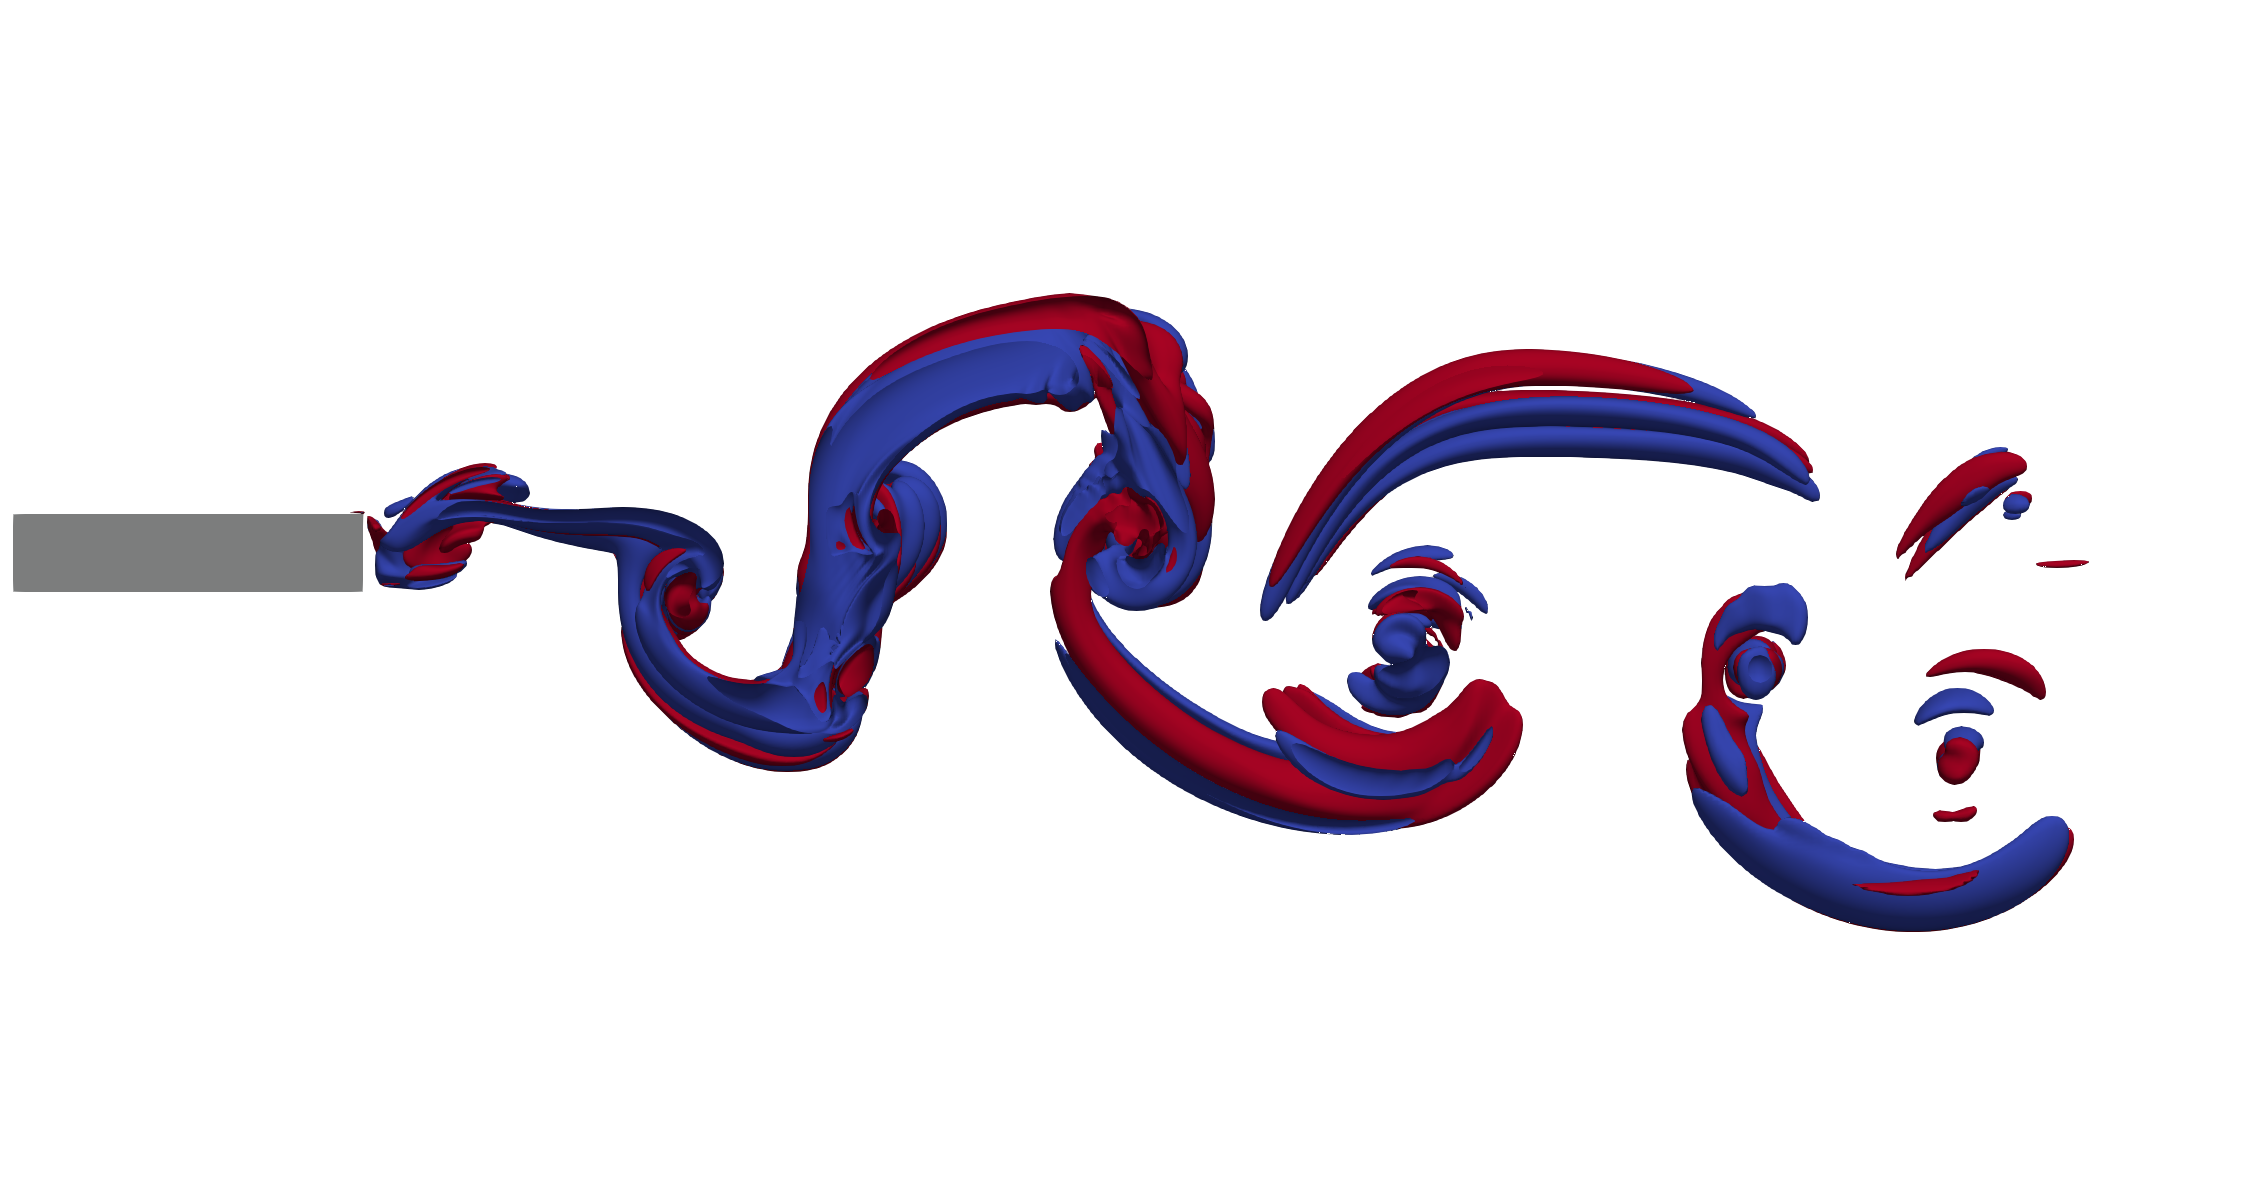
\includegraphics[trim={0 250 0 200},clip,width=0.49\textwidth]{./fig/AR4p5/omegax_Re475_2D.png}
  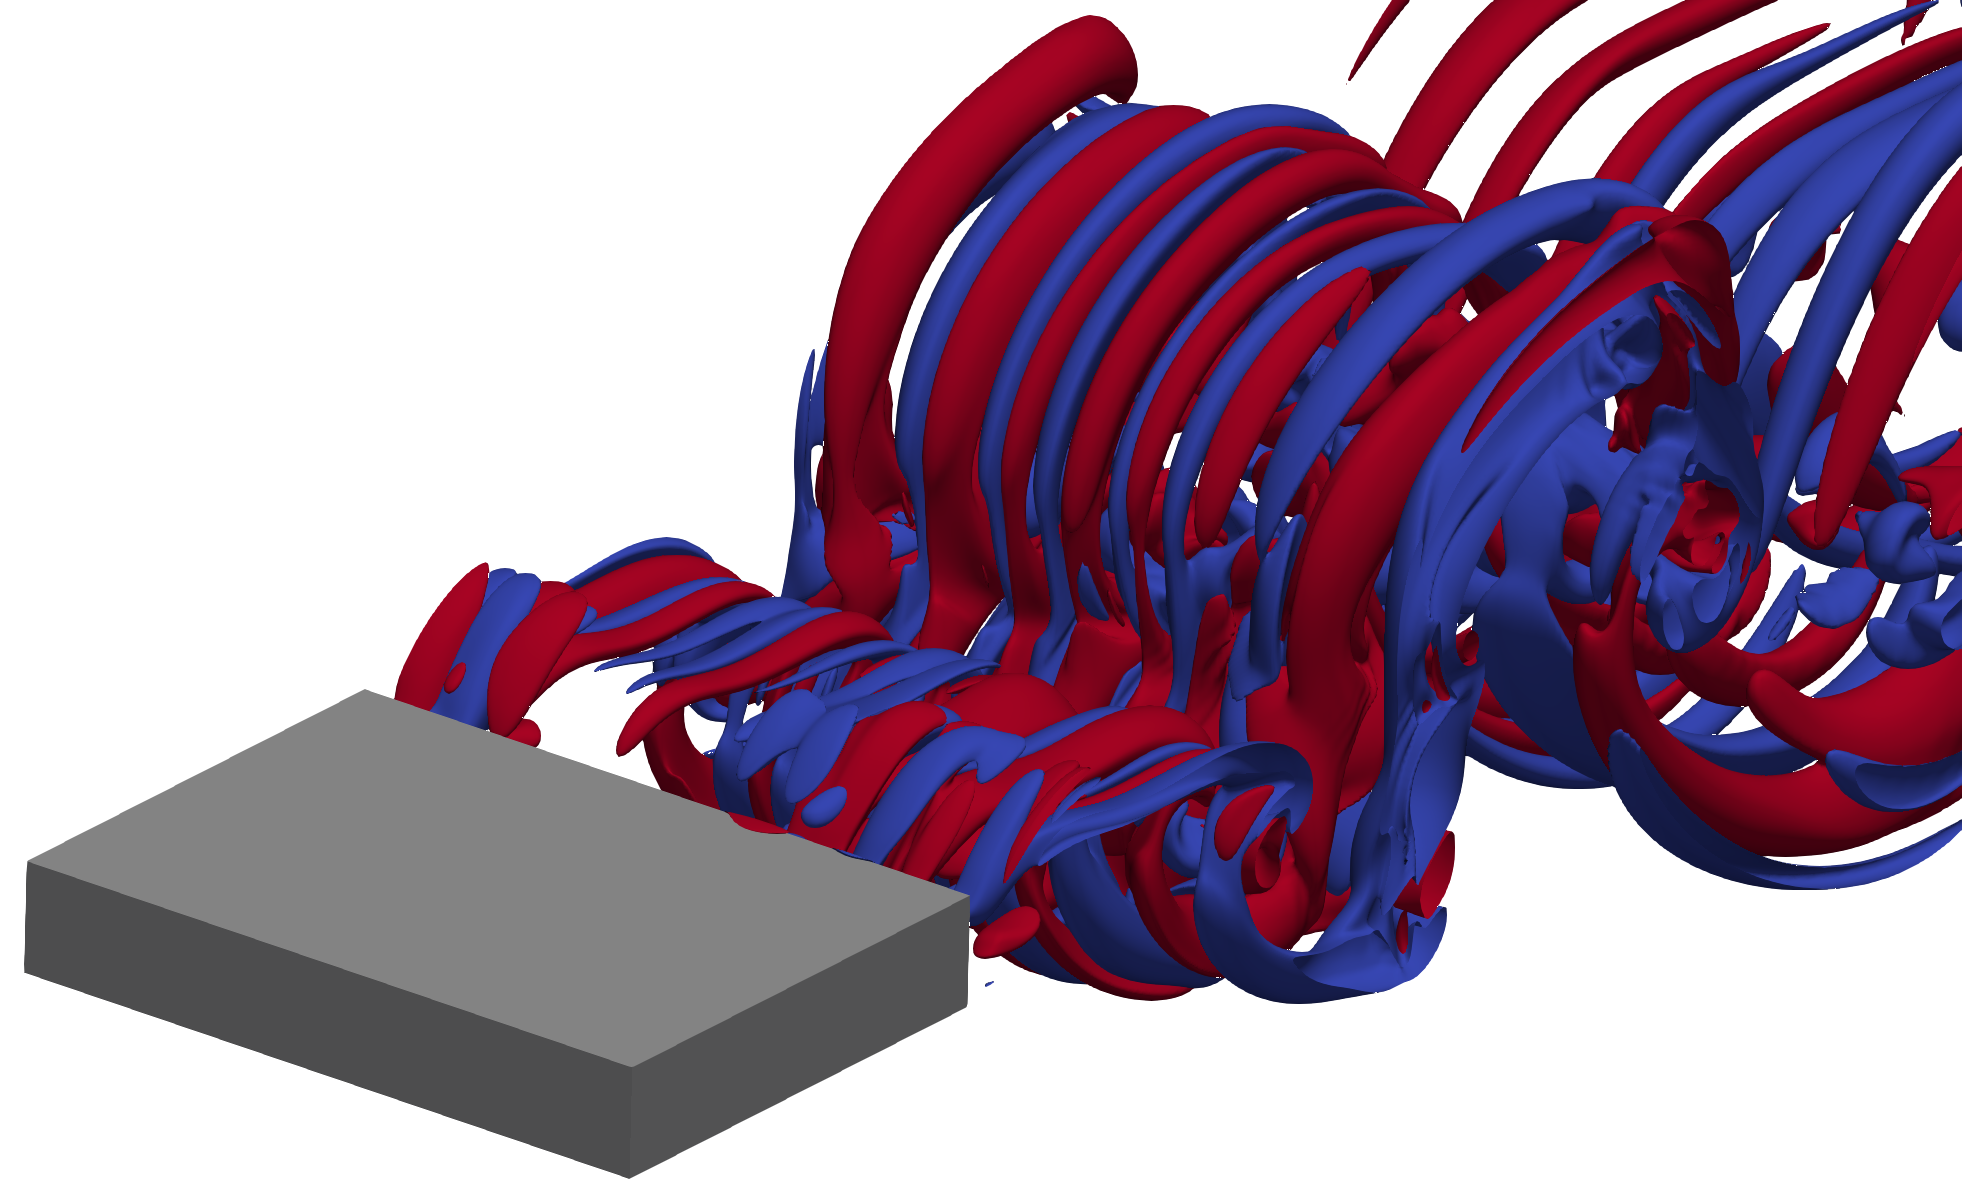
\includegraphics[trim={10 0 10 0},clip,width=0.49\textwidth]{./fig/AR4p5/omegax_Re475_3D.png} 
  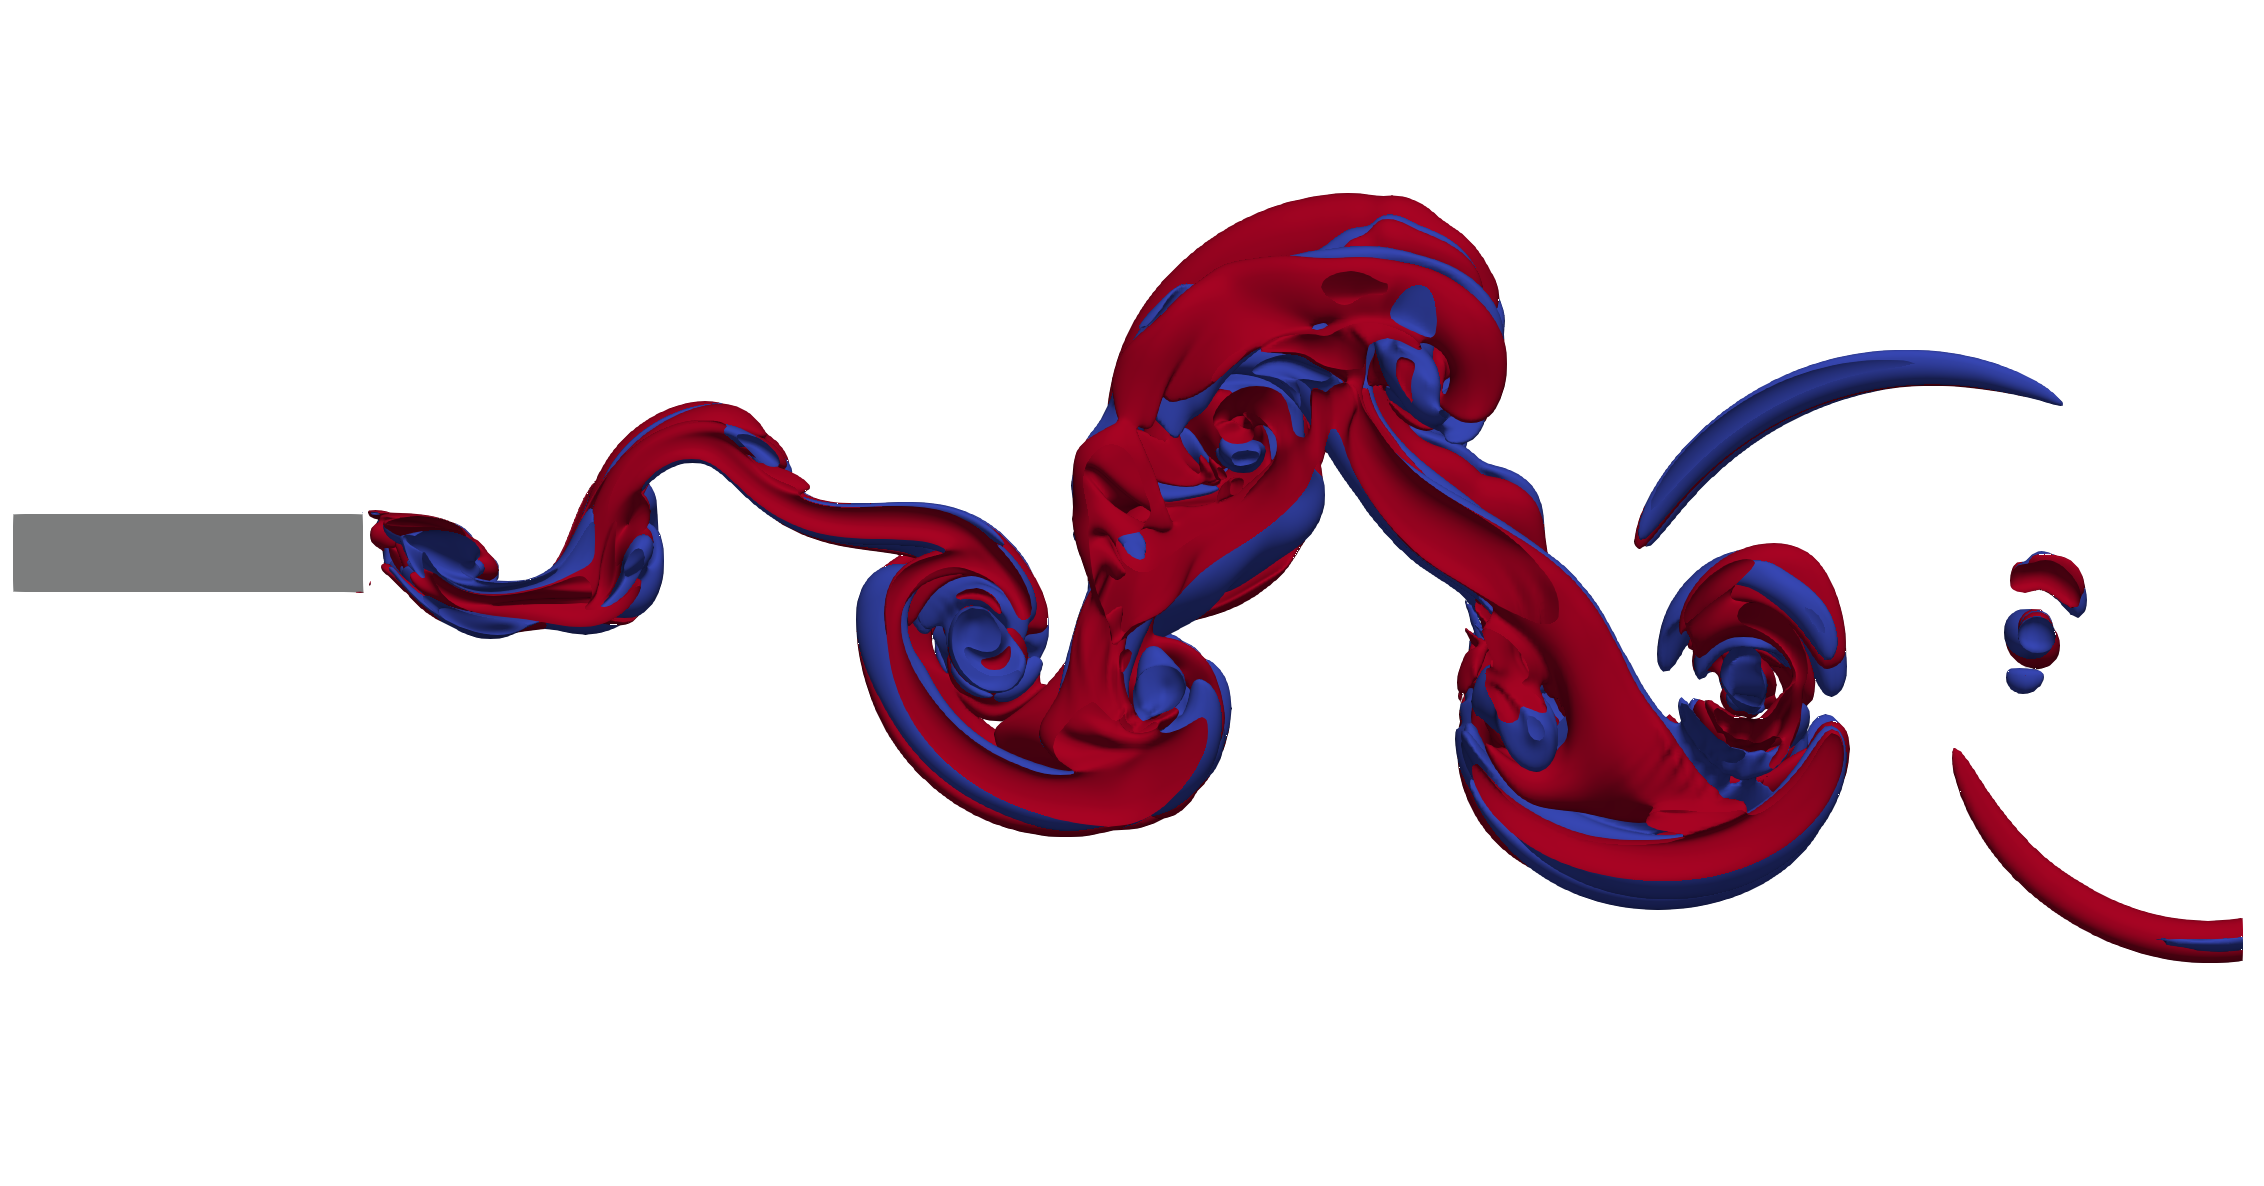
\includegraphics[trim={0 250 0 200},clip,width=0.49\textwidth]{./fig/AR4p5/omegax_Re500_2D.png}
  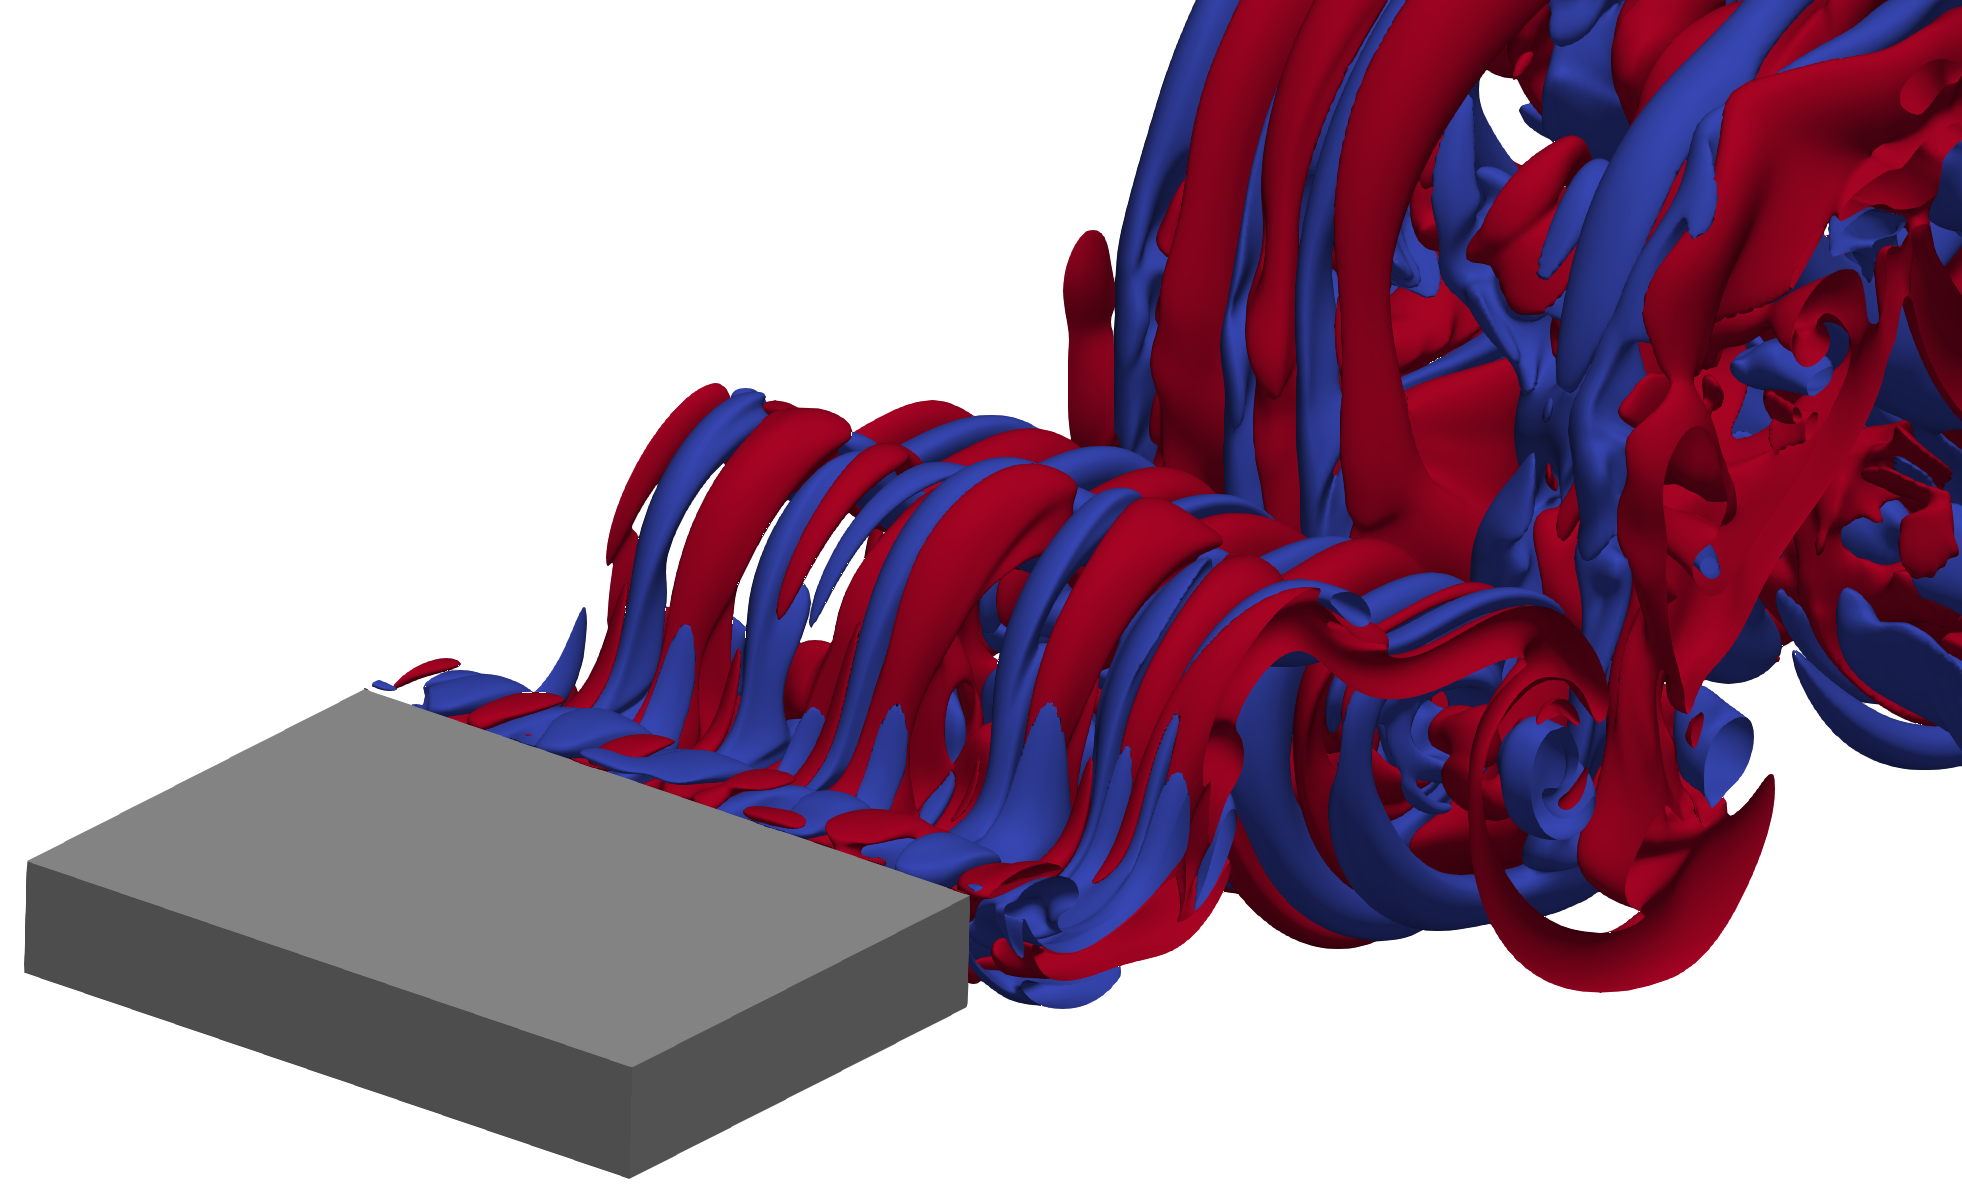
\includegraphics[trim={10 0 10 0},clip,width=0.49\textwidth]{./fig/AR4p5/omegax_Re500_3D.png} 
  \caption{Visualisation from direct numerical simulations for $\AR=4.5$. From top to bottom the Reynolds number is $Re=425,450,475$ and $500$. Left: lateral view. Right: three-dimensional view. The red/blue surfaces denote $\omega_x = \pm 0.25$.}
  \label{fig:viewdns-ar4p5}       
\end{figure}


\begin{figure}
  \centering
  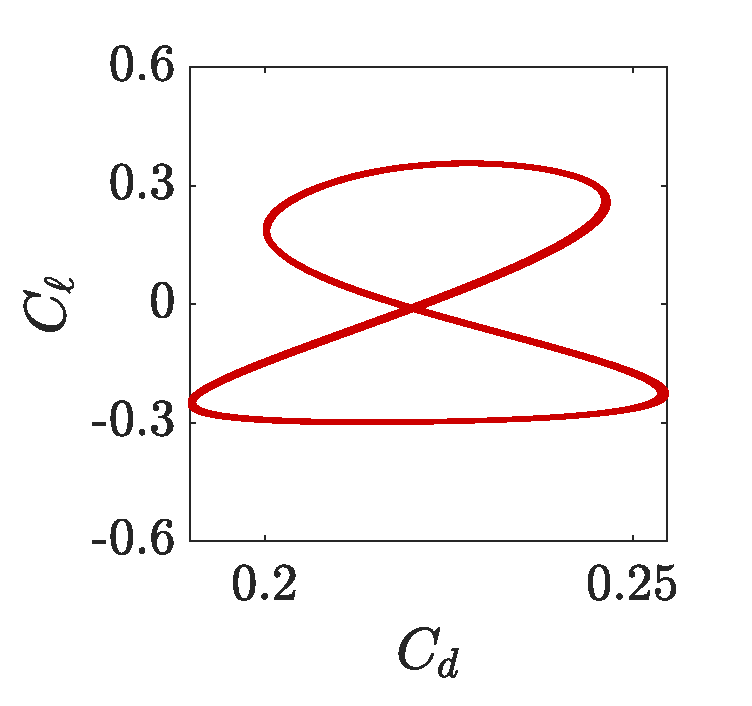
\includegraphics[width=0.325\textwidth]{./fig/AR4p5/Cl_Cd_Re425.eps}
  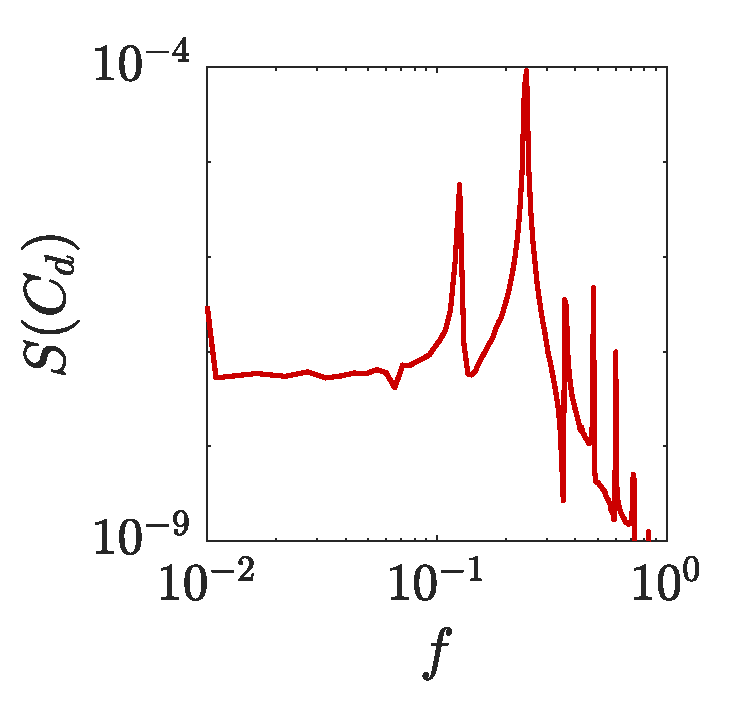
\includegraphics[width=0.325\textwidth]{./fig/AR4p5/Cd_f_Re425.eps}
  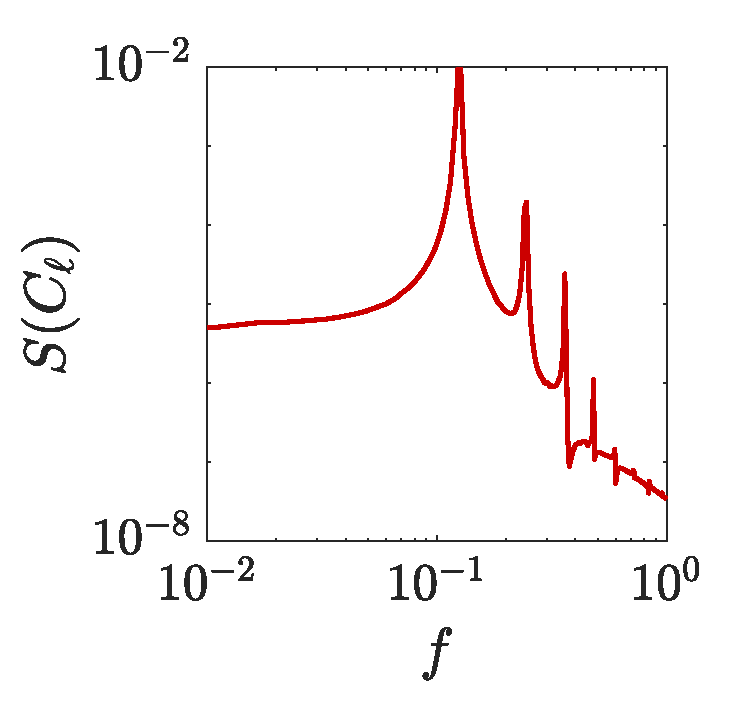
\includegraphics[width=0.325\textwidth]{./fig/AR4p5/Cl_f_Re425.eps} 
  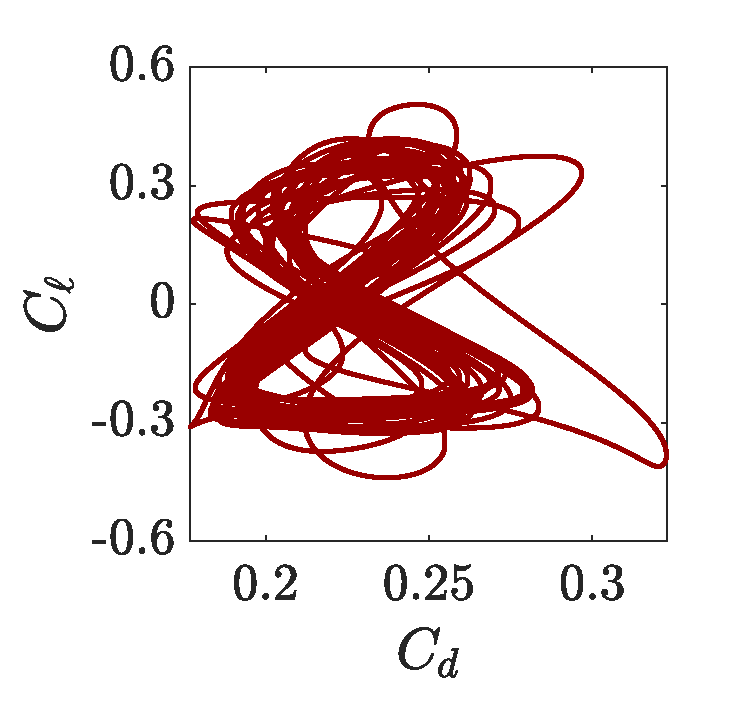
\includegraphics[width=0.325\textwidth]{./fig/AR4p5/Cl_Cd_Re450.eps}
  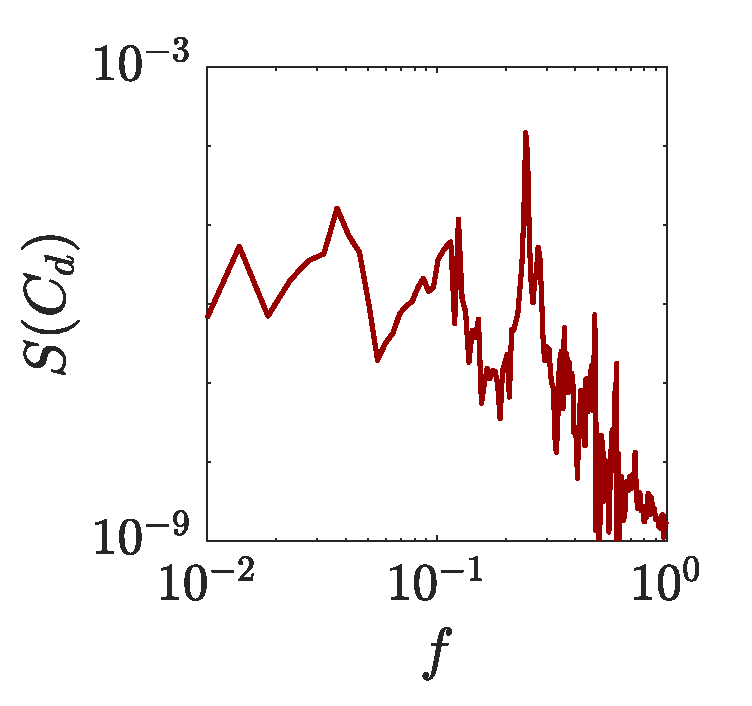
\includegraphics[width=0.325\textwidth]{./fig/AR4p5/Cd_f_Re450.eps}
  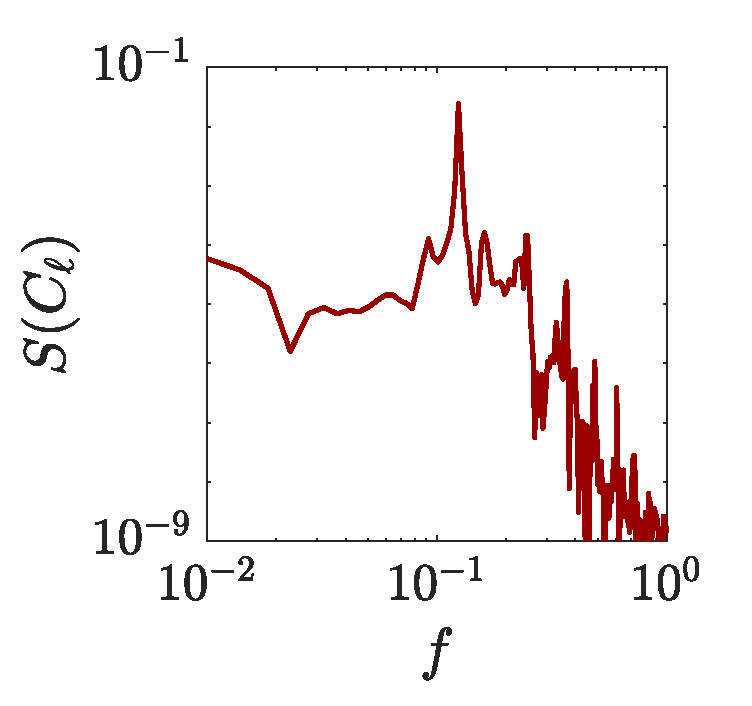
\includegraphics[width=0.325\textwidth]{./fig/AR4p5/Cl_f_Re450.eps} 
  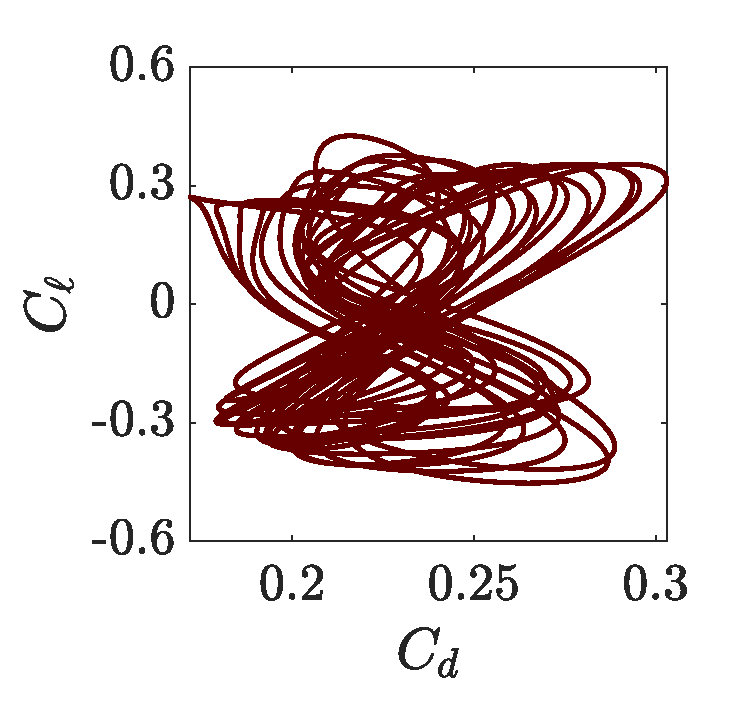
\includegraphics[width=0.325\textwidth]{./fig/AR4p5/Cl_Cd_Re475.eps}
  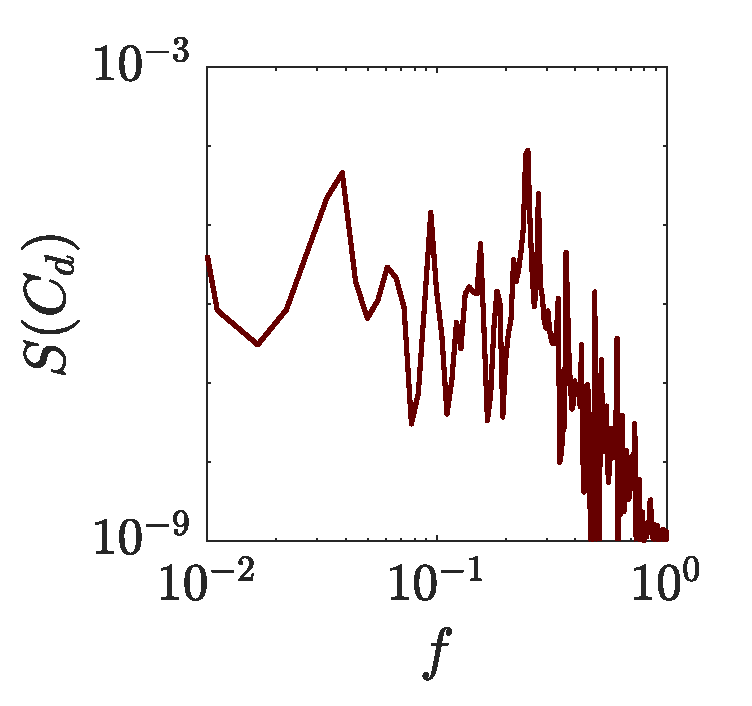
\includegraphics[width=0.325\textwidth]{./fig/AR4p5/Cd_f_Re475.eps}
  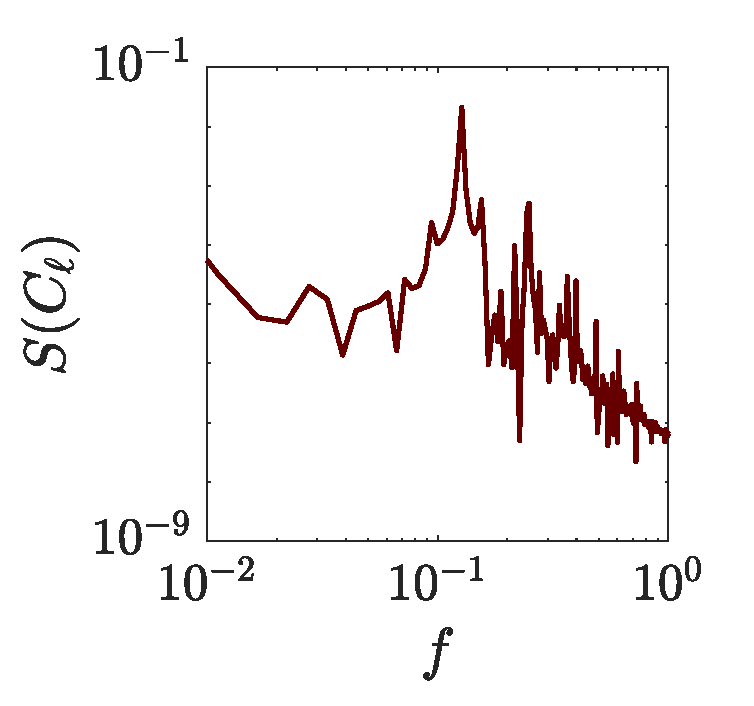
\includegraphics[width=0.325\textwidth]{./fig/AR4p5/Cl_f_Re475.eps}     
  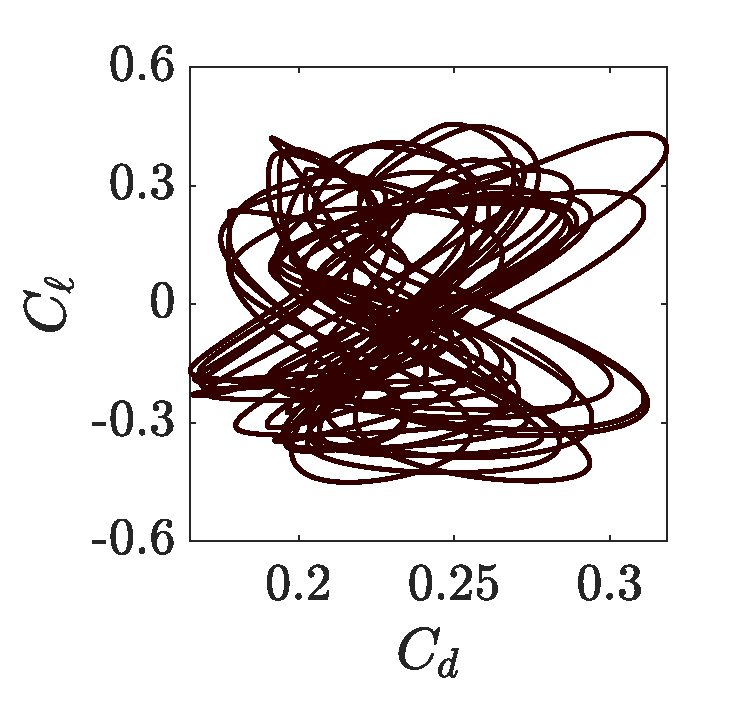
\includegraphics[width=0.325\textwidth]{./fig/AR4p5/Cl_Cd_Re500.eps}
  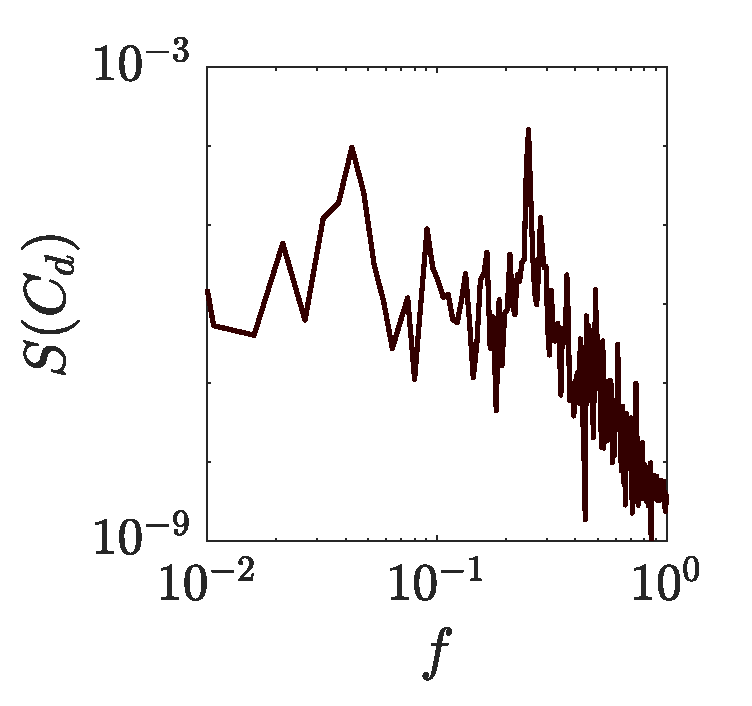
\includegraphics[width=0.325\textwidth]{./fig/AR4p5/Cd_f_Re500.eps}
  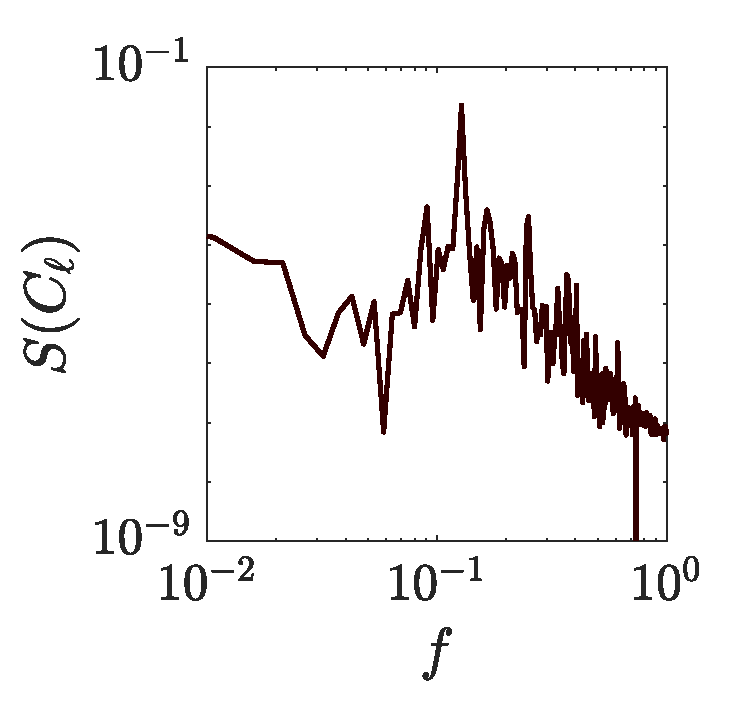
\includegraphics[width=0.325\textwidth]{./fig/AR4p5/Cl_f_Re500.eps}      
  \caption{Frequency content of the DNS simulations for $\AR=4.5$. From top to bottom the panels are for $Re=425,450,475$ and $500$. Left: $C_\ell-C_d$ maps. Centre: spectrum of $C_\ell$. Right: spectrum of $C_d$. \textcolor{red}{XX TO UPDATE AFTER THE SIMULATIONS HAVE CONVERGED XX}}
  \label{fig:clcddns-ar4p5}
\end{figure} 

Three-dimensional direct numerical simulations have been performed to extend the results of the Floquet stability analysis and to assess the influence of nonlinear effects on the flow dynamics. The aspect ratio is fixed at $\AR = 4.5$, and the Reynolds number is varied within the range $425 \le Re \le 500$, i.e. above the critical threshold $Re_{c3} \approx 420$ identified via Floquet analysis. The simulations are initialised from a 2D potential flow solution constructed using the Hess-Smith panel method, ensuring an unambiguous evolution toward the underlying attractor. Instantaneous flow visualisations are shown in figure~\ref{fig:viewdns-ar4p5}, while figure~\ref{fig:clcddns-ar4p5} highlights the nature of the attractor and the dominant flow scales.

At these parameters, the DNS confirm that the flow develops a deflected wake and acquires a fully 3D structure, as illustrated in figure~\ref{fig:viewdns-ar4p5}. Isocontours of the streamwise vorticity reveal a distinct spanwise modulation with a dominant wavenumber $\beta \approx 7$, in good agreement with the most amplified mode predicted by linear Floquet analysis. Notably, no significant 3D structures are observed near the lateral edges of the cylinder, indicating that the instability is confined to the wake and not driven by the LE vortex dynamics.

For $Re = 425$, the flow remains coherent and periodic, but progressively transitions to a more chaotic state as $Re$ increases, while preserving both the spanwise wavelength and the deflected configuration. This transition is evident in the $\omega_x$ isocontours in figure~\ref{fig:viewdns-ar4p5}, which gradually lose coherence. The spectra of the aerodynamic forces, shown in figure~\ref{fig:clcddns-ar4p5}, support this view. At $Re = 425$, the attractor traces a closed loop in phase space, and the lift-drag diagram exhibits a characteristic ``figure-eight'' shape, consistent with the drag oscillating at twice the frequency of the lift. The corresponding spectrum displays a dominant frequency $f \approx 0.13$ and its harmonics, matching the frequency of the $2D$ deflected base flow—indicative of a synchronous instability.

As $Re$ increases, the flow becomes aperiodic via a Neimark-Sacker bifurcation, introducing two incommensurate frequencies ($f_1 \approx 0.13$ and $f_2 \approx 0.09$), and the attractor evolves into a torus in phase space. Despite the onset of quasiperiodicity, the dominant spanwise wavelength of the $3D$ structures remains largely unchanged (figure~\ref{fig:viewdns-ar4p5}). At higher $Re$, additional spectral peaks emerge, including a low-frequency component near $f \approx f_1 - f_2$, arising from nonlinear interactions between the dominant modes, and the flow becomes increasingly chaotic.

The appearance of the new frequency for $Re \ge 450$ can be traced to a $2D$ Neimark–Sacker bifurcation of the deflected base flow. Linear stability analysis of this base flow reveals a complex-conjugate Floquet multiplier at $\beta = 0$ crossing the unit circle at $Re \approx 440$ (see figure~\ref{fig:AR4p5_modes_Re430_beta0}). At this Reynolds number, the base-flow period is $T \approx 8.31$, corresponding to $f \approx 0.12$, and the unstable multiplier $\mu = 0.815 + i 0.575$ corresponds to a secondary frequency $f \approx 0.077$, closely matching the low-frequency component observed in DNS at $Re = 450$.

In summary, for $Re \ge Re_{c3}$ the flow becomes $3D$, characterised by a spanwise wavelength $\lambda_z \approx 0.89$ and a persistent deflected configuration. For $Re < Re_{c4} \approx 440$, the flow remains periodic, with a dominant frequency matching that of the 2D base flow. At $Re \ge Re_{c4}$, a Neimark-Sacker bifurcation induces a transition to quasiperiodicity, followed by a progressive increase in spectral complexity and flow irregularity.


